\chapter[Properties of Pristine and Hydrogenated Beryllene]{Emergent Topological, Superconducting, and Optical Properties of Pristine and Hydrogenated Beryllene Phases}
\label{cha:project_beryllene}

This chapter is based on the manuscript by L.~Niu, O.~J.~Conquest, H.~Ma, C.~Verdi, and C.~Stampfl~\cite{niu2026draftemergent}.
The candidate carried out the \texttt{VASP} and postprocessing calculations, data analysis, and visualization.
Catherine Stampfl supervised the project.
Oliver James Conquest provided detailed guidance on the calculations.
Hongyang Ma performed the \texttt{Quantum ESPRESSO} and \texttt{EPW} calculations.
Carla Verdi performed the validation.
All authors contributed to writing or revising the manuscript.

\section{Abstract}
\label{3_abstract}

We use density functional theory to compare the stability, electronic structure, band topology, superconductivity, and optical response of pristine and hydrogen-functionalized beryllene.
Starting from three (001) layers of bulk body-centred cubic beryllium, we obtain trilayer cubic beryllene, an ABA-stacked structure with a square lattice.
Its calculated harmonic phonon frequencies are real along the sampled path.
When hydrogen terminates both faces of monolayer $\alpha$-beryllene, HSE06 gives an indirect gap of \qty{6.00}{\electronvolt}.
Bilayer $\beta$-beryllene remains metallic with hydrogen on one or both faces.
At \qty{298.15}{\kelvin} and a hydrogen pressure of \qty{1}{\bar}, the calculated adsorption free energy is negative only for the doubly terminated $\alpha$ phase.
Across the sampled visible range, the cubic trilayer has a smaller in-plane interband absorption coefficient than its bulk parent.
Hydrogenation also splits the two in-plane optical responses of $\beta$-beryllene.
The lowest six spinor bands of trilayer cubic beryllene give a conditional $\mathbb{Z}_2$ index of $\nu=1$.
The smallest sampled direct gap separating this subspace from the higher bands is \qty{0.735}{\milli\electronvolt} and occurs about \qty{1.2}{\electronvolt} above the Fermi level.
The lowest two spinor bands of pristine $\alpha$-beryllene also give $\nu=1$.
These indices describe band subspaces in two metals.
The selected subspaces of the hydrogenated structures give $\nu=0$.
Electron-phonon calculations predict phonon-mediated superconductivity in the cubic trilayer and both hydrogen-functionalized $\beta$ phases.
The highest anisotropic Migdal--Eliashberg transition temperature is approximately \qty{31.7}{\kelvin} for double-sided hydrogen-terminated $\beta$-beryllene relaxed with the D3 dispersion correction.

\section{Introduction}
\label{3_introduction}

Reducing an elemental crystal to a few atomic layers changes the coordination of its atoms and the symmetry of its lattice.
Graphene is a familiar example in which the two-dimensional lattice gives rise to Dirac fermions~\cite{novoselov2004electric,geim2007rise}.
Other elemental two-dimensional materials, known as Xenes, let us examine changes in bonding and electronic structure within a single element~\cite{molle2018silicene}.
For beryllium, we ask which few-layer structures retain their atomic framework and how hydrogen termination changes their electronic and optical properties.

First-principles calculations predicted hexagonal beryllium monolayers and bilayers~\cite{ono2020dynamical,hess2022periodicity}.
Chahal et al. subsequently obtained beryllene sheets by sonochemical exfoliation of elemental beryllium powder~\cite{chahal2023beryllene}.
High-resolution transmission electron microscopy revealed hexagonal and square-like lattice geometries, and electrical measurements gave a metallic response.
The square-like lattice constrains the in-plane geometry but leaves the stacking sequence open.
For the hexagonal monolayer, Chowdhury and Mogurampelly predicted a lattice thermal conductivity of approximately \qty{270}{\watt\per\metre\per\kelvin} at room temperature~\cite{chowdhury2024unusual}.
They attributed the large in-plane conductivity to weak phonon scattering and a substantial contribution from long-wavelength flexural modes.

Li et al. identified Dirac-like crossings arising from Be $s$ and $p$ states in the hexagonal monolayer and bilayer~\cite{li2023coexistence}.
These two structures are known as $\alpha$-beryllene and $\beta$-beryllene.
Electron-phonon calculations for these phases predict superconducting transition temperatures of the order of \qty{10}{\kelvin}~\cite{li2023coexistence}.
Derriche et al. showed that orbital hybridization and lattice symmetry can generate non-trivial band topology in light-element systems with weak spin-orbit coupling~\cite{derriche2024light}.
These results motivate a comparison of band order and pairing across beryllene structures with different coordination.
Low-temperature transport measurements on ultrathin beryllium films also show superconducting correlations and strong disorder effects~\cite{xiong2009spin}.

Structural changes and adsorbates can alter band topology in elemental layers.
For example, interlayer sliding can switch the calculated topology of a bismuth bilayer~\cite{qian2025switchable}.
In monolayer arsenene, calculations predict a quantum spin Hall state under hydrogenation and strain~\cite{zhang2016controllable}.
For beryllium, previous calculations found that hydrogen favours high-symmetry sites on the Be(0001) surface and induces local lattice relaxation~\cite{bachurin2015ab}.
A separate structure search predicted wide-gap beryllium hydride monolayers with multicentre Be-H bonding~\cite{li2018global}.
We therefore examine hydrogen as a surface termination and test whether the underlying beryllium framework persists.

We compare the two hexagonal phases with trilayer cubic beryllene, an ABA-stacked trilayer with a square lattice.
We denote double-sided hydrogen-terminated $\alpha$-beryllene by 2H-$\alpha$-beryllene.
For the $\beta$ phase, we denote the single- and double-sided configurations by 1H-$\beta$-beryllene and 2H-$\beta$-beryllene, respectively.
Section~\ref{3_methods} describes the calculation methods.
Section~\ref{3_results} starts with the structures, their dynamical stability, and the energetics of hydrogen adsorption.
We then examine their electronic bands, band topology, electron-phonon coupling, and optical response.
Section~\ref{3_supplementary} provides the convergence tests and additional results.

\section{Computation methods}
\label{3_methods}

We perform density functional theory calculations with the Vienna Ab initio Simulation Package (\texttt{VASP})~\cite{kresse1993ab,kresse1994ab,kresse1996efficiency,kresse1996efficient}.
We describe the electron-ion interaction with the projector augmented wave method~\cite{kresse1999ultrasoft}.
For exchange and correlation, we use the Perdew--Burke--Ernzerhof (PBE) generalized gradient approximation~\cite{perdew1996generalized}.
The \texttt{VASP} structural relaxations, total energies, reported phonon spectra, and molecular dynamics simulations use PBE without a dispersion correction.
We include the D3 dispersion correction with Becke--Johnson damping in the PBE band calculations without spin-orbit coupling~\cite{becke2005density,grimme2010consistent,grimme2011effect}.
At a fixed geometry, this correction changes the total energy and leaves the Kohn--Sham eigenvalues unchanged.
We calculate these bands non-self-consistently.
For metals, we reference the bands to the Fermi level of the corresponding self-consistent calculation.
For 2H-$\alpha$-beryllene, we align the plotted bands at their valence-band maximum.

For the bulk hexagonal close-packed (hcp) and body-centred cubic (bcc) reference phases, we use a $\Gamma$-centred $27 \times 27 \times 27$ k-point mesh for structural relaxations and total energies.
The dielectric function uses a $105 \times 105 \times 105$ mesh.
We use a plane-wave cutoff of \qty{600}{\electronvolt}, except in the molecular dynamics simulations described below.
We converge the electronic energy to \qty{1e-6}{\electronvolt} and relax the structures until the force on each atom falls below \qty{0.001}{\electronvolt\per\angstrom}.
For the two-dimensional structures, we fix the supercell height normal to the layers at \qty{40}{\angstrom} and apply a dipole correction along this direction~\cite{neugebauer1992adsorbate}.
We relax the in-plane lattice vectors and atomic positions using $27 \times 27 \times 1$ meshes for the hexagonal phases and their hydrogenated derivatives.
For the cubic structures, we use $25 \times 25 \times 1$ meshes.
We use a $105 \times 105 \times 1$ mesh for the dielectric functions of all two-dimensional structures.
Figures~\ref{fig:proj3_cohesive_energy_convergence}--\ref{fig:proj3_cubic_dielectric_kpoint_convergence} give the convergence tests for the cohesive energies, total energies, and dielectric functions.
Separate series test the sensitivity of the dielectric function to the k-point mesh and to the number of bands.

For bulk hcp beryllium, $\alpha$-beryllene, bulk bcc beryllium, and trilayer cubic beryllene, the cohesive energies on the selected and densest k-point meshes differ by at most \qty{0.3}{\milli\electronvolt} per atom.
The densest meshes are $41 \times 41 \times 41$ for the bulk phases and $47 \times 47 \times 1$ for the two-dimensional phases.
Across all denser meshes tested, the cohesive energies differ from those on the selected meshes by at most \qty{2.2}{\milli\electronvolt} per atom.

We calculate the harmonic phonon dispersions with \texttt{phonopy} using finite displacements of \qty{0.01}{\angstrom}~\cite{togo2015first,togo2023implementation}.
We use $5 \times 5 \times 1$ supercells for the two-dimensional phases except the cubic trilayer, for which we use a $4 \times 4 \times 1$ supercell.
For bulk hcp and bcc beryllium, the supercells are $4 \times 4 \times 3$ and $4 \times 4 \times 4$, respectively.
The force calculations use Gaussian smearing of \qty{0.05}{\electronvolt} and an electronic convergence criterion of \qty{1e-8}{\electronvolt}.
For the metallic two-dimensional phases, the supercell meshes correspond to approximately $65 \times 65$ k points per unit cell.
The relaxed cells of $\alpha$-beryllene and 2H-$\alpha$-beryllene deviate from hexagonal symmetry by up to \qty{1e-4}{\angstrom}.
We use a symmetry tolerance of \qty{1e-3}{\angstrom} to recover equivalence among the supercell images used in the interpolation.
We include D3 in the preliminary phonon screening and use uncorrected PBE for the finite-displacement dispersions reported here.
We use frozen-phonon calculations to examine the soft mode of 2H-$\beta$-beryllene in section~\ref{3_supplementary}.

We examine the hydrogen-functionalized structures at finite temperature with \textit{ab initio} molecular dynamics (AIMD).
These simulations use $5 \times 5 \times 1$ supercells without the dipole correction.
The supercell height is \qty{26.7}{\angstrom} for 2H-$\alpha$-beryllene and \qty{40}{\angstrom} for both hydrogenated $\beta$ structures.
We use the canonical (NVT) ensemble with a Nos\'e--Hoover thermostat at \qty{300}{\kelvin}~\cite{nose1984unified,hoover1985canonical}.
Each simulation runs for \qty{5.5}{\pico\second} with a time step of \qty{0.5}{\femto\second}.
The plane-wave cutoff is \qty{350}{\electronvolt} and the k-point mesh is $3 \times 3 \times 1$.

To compare each hydrogenated layer with its pristine counterpart and molecular hydrogen, we define the adsorption energy per hydrogen atom $E_{\mathrm{ad}}$ as:
\begin{equation}
    E_{\mathrm{ad}} \coloneqq
    \frac{E_{\mathrm{H/Be}}-E_{\mathrm{Be}}-n_{\mathrm{H}}E_{\mathrm{H}}}{n_{\mathrm{H}}}
\label{eq:proj3_hydrogen_adsorption_energy}
\end{equation}

here, $E_{\mathrm{H/Be}}$ and $E_{\mathrm{Be}}$ are the total energies of the hydrogenated and pristine unit cells, respectively.
$E_{\mathrm{H}}$ is half the total energy of an isolated \ce{H2} molecule and $n_{\mathrm{H}}$ counts the hydrogen atoms in the hydrogenated unit cell.
A negative $E_{\mathrm{ad}}$ means that adsorption lowers the electronic energy relative to the pristine layer and gaseous hydrogen.

We include zero-point motion by adding the harmonic zero-point energy to each total energy in equation~\eqref{eq:proj3_hydrogen_adsorption_energy}.
For the layers, we obtain these energies from phonons on a $40 \times 40$ q-point mesh and omit imaginary modes.
The calculated molecular stretching wavenumber of \ce{H2} is \qty{4341}{\per\centi\metre}.
This wavenumber gives a zero-point energy of \qty{0.269}{\electronvolt} per molecule, of which half is subtracted per adsorbed hydrogen atom.
At \qty{298.15}{\kelvin} and a hydrogen pressure of \qty{1}{\bar}, we use the harmonic vibrational free energies of the layers and include the enthalpy and entropy changes of gaseous \ce{H2} from the NIST-JANAF tables~\cite{chase1998nist}.

To compare the bonding in the pristine structures, we define the cohesive energy per beryllium atom $E_{\mathrm{c}}$ as:
\begin{equation}
    E_{\mathrm{c}} \coloneqq
    \frac{E_{\mathrm{Be\text{-}struc}}-n_{\mathrm{Be}}E_{\mathrm{Be\text{-}atom}}}{n_{\mathrm{Be}}}
\label{eq:proj3_cohesive_energy}
\end{equation}

here, $E_{\mathrm{Be\text{-}struc}}$ is the total energy of a unit cell containing $n_{\mathrm{Be}}$ atoms.
$E_{\mathrm{Be\text{-}atom}}$ is the total energy of an isolated beryllium atom in a large supercell.
The cohesive energy measures the energy change per atom upon assembling the structure from isolated atoms.

For the topological calculations, we keep the supercell height of \qty{40}{\angstrom} and the dipole correction.
We use a plane-wave cutoff of \qty{600}{\electronvolt}, a $105 \times 105 \times 1$ k-point mesh, Gaussian smearing of \qty{0.01}{\electronvolt}, and an electronic convergence criterion of \qty{1e-8}{\electronvolt}.
We include spin-orbit coupling in the band and parity calculations.
We calculate the parities of the spinor states with \texttt{IrRep}~\cite{iraola2022irrep} and check them against the inversion matrix reconstructed from the wave functions in double precision.
At a time-reversal invariant momentum $\vec{\Lambda}_i$, we take one parity eigenvalue from each Kramers pair to form the parity product:
\begin{equation}
    \delta_i =
    \prod_{m=1}^{N/2}
    \xi_{2m}(\vec{\Lambda}_i\,)
\label{eq:proj3_parity_product}
\end{equation}

here, $\xi_{2m}(\vec{\Lambda}_i\,)=\pm1$ is the parity eigenvalue of one state in pair $m$.
$N$ is the number of spinor bands in the selected subspace, so $N=2N_\mathrm{p}$ in the notation of chapter~\ref{cha:fundamentals_c}.
We take the product over $\Gamma=(0,0)$, $\mathrm{X}=(1/2,0)$, $\mathrm{Y}=(0,1/2)$, and $\mathrm{M}=(1/2,1/2)$ in reciprocal lattice coordinates.
This product gives the Fu--Kane relation for the $\mathbb{Z}_2$ index~\cite{fu2007topological,fu2007topological3d}:
\begin{equation}
    (-1)^{\nu} =
    \prod_{i=1}^{4} \delta_i
\label{eq:proj3_z2_index}
\end{equation}

here, $\nu=1$ denotes non-trivial topology, whereas $\nu=0$ denotes trivial topology.
Sections~\ref{sec:fu_kane_criterion_topology} and~\ref{sec:interpreting_topology_calculation} derive the criterion and describe its application to an isolated band subspace.
The 1H-$\beta$-beryllene structure lacks inversion symmetry.
We therefore obtain $\nu$ from the evolution of Wannier charge centres across half of the Brillouin zone~\cite{soluyanov2011computing,gresch2017z2pack}.
We calculate the centres with \texttt{Z2Pack} from spinor overlaps exported through the \texttt{VASP} interface to \texttt{Wannier90}~\cite{pizzi2020wannier90}.
The final set of 23 Wilson loops passes the convergence checks in \texttt{Z2Pack}.
In the metallic structures, we check the isolation of the lowest $N$ bands through the direct gap $E_{N+1}(\vec{k}\,)-E_N(\vec{k}\,)$.
We sample this gap on the $105 \times 105$ mesh and along the band paths, then refine the meshes around the minima.
We also check for magnetic solutions by starting spin-polarized calculations from ferromagnetic and antiferromagnetic configurations.

To test the PBE band gap and ordering, we use the HSE06 hybrid functional~\cite{heyd2003hybrid,krukau2006influence}.
These calculations use a supercell height of \qty{20}{\angstrom} and a $\Gamma$-centred $12 \times 12 \times 1$ mesh for both the electronic states and the Fock exchange.
We omit spin-orbit coupling in the hybrid calculations.
Inversion acts on the spatial part of the wave function.
We therefore compare the spinless parities with those of the PBE Kramers pairs at the time-reversal invariant momenta.
For 2H-$\alpha$-beryllene, we sample 71 points along $\Gamma$--$\mathrm{K}$--$\mathrm{M}$--$\Gamma$ and 9 additional points around each PBE band edge.

For the \texttt{Quantum ESPRESSO} calculations, we use the PBE relaxed structures~\cite{giannozzi2017advanced,giannozzi2009quantum}, with a separate relaxation for the phonon and electron-phonon calculations of 2H-$\beta$-beryllene.
We use optimized norm-conserving Vanderbilt pseudopotentials that treat the Be $1s$ states as valence states~\cite{hamann2013optimized}.
The plane-wave cutoffs are \qty{80}{Ry} for the wave functions and \qty{640}{Ry} for the charge density.
We use Marzari--Vanderbilt smearing of \qty{0.02}{Ry} and a two-dimensional Coulomb cutoff with at least about \qty{15}{\angstrom} of vacuum~\cite{marzari1999thermal,sohier2017density}.
The self-consistent k-point meshes are $56 \times 56 \times 1$ for trilayer cubic beryllene, $52 \times 52 \times 1$ for 2H-$\alpha$-beryllene, $46 \times 46 \times 1$ for 2H-$\beta$-beryllene, and $57 \times 52 \times 1$ for 1H-$\beta$-beryllene in the input lattice-vector order.
Table~\ref{tab:proj3_qe_structures} lists these structures.
For the parity calculations, we use fully relativistic projector augmented wave pseudopotentials with spin-orbit coupling and cutoffs of \qty{90}{Ry} and \qty{720}{Ry}~\cite{dalcorso2014pseudopotentials}.
For the Wilson loops~\cite{yu2011equivalent}, we build models with \texttt{Wannier90} and evaluate them with \texttt{WannierTools}~\cite{pizzi2020wannier90,wu2018wanniertools}.

We calculate the phonons of trilayer cubic beryllene, 2H-$\beta$-beryllene, and 1H-$\beta$-beryllene by density functional perturbation theory on a $12 \times 12 \times 1$ q-point mesh~\cite{baroni2001phonons}.
We use \texttt{EPW} for the electron-phonon calculations~\cite{lee2023electron,giustino2007electron}.
For 2H-$\beta$-beryllene, we include D3 with Becke--Johnson damping and use the structure relaxed with this correction, with a lattice constant of \qty{2.53}{\angstrom}.
We initialize the Wannier functions with Be $s$ and $p$ and H $s$ projections and exclude the Be $1s$ bands.
We interpolate the electronic states and phonon perturbations from coarse $24 \times 24 \times 1$ k-point and $12 \times 12 \times 1$ q-point meshes onto fine $80 \times 80 \times 1$ meshes.
We compare the results with calculations on $40 \times 40 \times 1$ meshes.
The electronic and phonon smearings are \qty{0.15}{\electronvolt} and \qty{0.5}{\milli\electronvolt}, respectively.
We include electronic states within \qty{0.6}{\electronvolt} of the Fermi level and use a Matsubara energy cutoff of \qty{1.2}{\electronvolt}.

For trilayer cubic beryllene and 2H-$\beta$-beryllene, we exclude phonons below \qty{40}{\per\centi\metre}, corresponding to about \qty{5}{\milli\electronvolt}.
On the $12 \times 12 \times 1$ q-point mesh, this range contains only the acoustic branches near $\Gamma$.
On the $40 \times 40 \times 1$ fine meshes, it contributes about half of the electron-phonon coupling strength $\lambda$.
Above the threshold, the $40 \times 40 \times 1$ and $80 \times 80 \times 1$ fine meshes give similar values of $\lambda$.
The reported $\lambda$ and transition temperatures of these two structures refer to phonons above the threshold.
For 1H-$\beta$-beryllene, modes below \qty{40}{\per\centi\metre} contribute less than \qty{1}{\percent} to $\lambda$.
We therefore use a smaller cutoff of \qty{5}{\per\centi\metre} for this structure.
Table~\ref{tab:proj3_epw_threshold} and figure~\ref{fig:proj3_a2f} compare the results for the two fine meshes and the two thresholds.
We obtain $\lambda$ and the logarithmic average frequency $\omega_\mathrm{log}$ from the Eliashberg spectral function $\alpha^2F(\omega)$ using equations~\eqref{eliashberg_spectral_function_method} and~\eqref{electron_phonon_spectral_moments}.

Firstly, we estimate the superconducting transition temperature $T_\mathrm{c}$ with the simplified Allen--Dynes expression~\eqref{allen_dynes_temperature_estimate} for Coulomb pseudopotentials $\mu^*$ from 0.10 to 0.16~\cite{allen-dynes,mcmillan1968transition}.
Secondly, we solve the isotropic Migdal--Eliashberg equations on the imaginary axis with $\mu^*=0.13$~\cite{giustino2017electron,eliashberg1960interactions,migdal1958interaction}.
We obtain the isotropic $T_\mathrm{c}$ by fitting the temperature dependence of the gap at the first Matsubara frequency.
For the two hydrogenated $\beta$ phases, we also solve the anisotropic Migdal--Eliashberg equations at each temperature using up to 6000 iterations~\cite{margine2013anisotropic}.
Near $T_\mathrm{c}$, the slow convergence requires us to track the gap through the iterations.
We classify a temperature as below $T_\mathrm{c}$ when each fitted range gives a non-zero limiting gap.
Above $T_\mathrm{c}$, the gap decays exponentially with the iteration count.
We estimate the transition by extrapolating the limiting gaps below $T_\mathrm{c}$ and the decay rates above it.

We calculate the optical spectra from PBE eigenvalues and transition matrix elements for all eight structures.
This common choice lets us compare their frequency-dependent dielectric tensors $\varepsilon_{\alpha\beta}(\omega)$ at the same level of theory.
Chapter~\ref{cha:fundamentals_b} derives the dielectric response, Kramers--Kronig relation, and optical quantities in sections~\ref{sec:from_electronic_response_to_dielectric_function} and~\ref{sec:from_dielectric_function_to_optical_properties}.
Here, we apply the scalar relations separately to the Cartesian diagonal components $\varepsilon_{\lambda\lambda}(\omega)$, with $\lambda=x,y,z$.
They give principal-component optical quantities for a diagonal tensor and a propagation geometry compatible with the chosen component.
For the lower-symmetry hydrogenated $\beta$ phases, the resulting spectra compare the diagonal responses without the off-diagonal coupling.
In particular, the scalar loss function $L_{\lambda}(\omega)$ uses $1/\varepsilon_{\lambda\lambda}(\omega)$, which can differ from the corresponding component of the inverse tensor.
The calculated reflectivity describes a homogeneous semi-infinite medium within the scalar normal-incidence approximation.

We use \texttt{LOPTICS=T} in \texttt{VASP} 6.5.0 for the independent-particle optical response.
We set \texttt{ISPIN=1} and \texttt{LSORBIT=F} to omit spin polarization and spin-orbit coupling.
We use Gaussian occupation smearing of \qty{0.01}{\electronvolt} with \texttt{ISMEAR=0} and \texttt{SIGMA=0.01}.
The complex frequency shift is \qty{0.1}{\electronvolt}, set by \texttt{CSHIFT=0.1}.
The spectra include interband transitions without microscopic local-field effects.
For metals, these spectra describe the interband part of the low-frequency response, as both the calculation with \texttt{WPLASMAI=0} and the postprocessing omit the Drude term.

The supercell dielectric tensor of a two-dimensional structure describes the response averaged over the layer and its surrounding vacuum.
We apply equation~\eqref{optical_volume_normalization_2d} with the full supercell height of \qty{40}{\angstrom} to obtain an effective response for the layer~\cite{yang2021method}.
The effective thickness $d_\mathrm{2D}$ is the separation between the outermost atomic centres along the normal plus the two outer atomic radii.
We use radii of \qty{1.98}{\angstrom} for Be and \qty{0.70}{\angstrom} for H.
The same normalization applies to the $xx$, $yy$, and $zz$ components, so the magnitude of the effective response depends on this thickness convention.
Section~\ref{3_supplementary} gives the thicknesses and the numbers of bands used.

\section{Results and discussion}
\label{3_results}

\subsection{Atomic structure}
\label{3_atomic_structure}

We start with bulk hcp and bcc beryllium as references for the two-dimensional phases.
Figures~\ref{fig:proj3_bulk_structures}, \ref{fig:proj3_pristine_2d_structures}, and~\ref{fig:proj3_hydrogenated_structures} show the bulk, pristine two-dimensional, and hydrogen-functionalized structures, respectively.

\begin{figure}[!htbp]
\centering
    
\includegraphics[width=1.00\linewidth]{figures_proj3/structure_bulk_thesis.pdf}
\caption{Atomic structures of the bulk beryllium phases.
Left and middle: top and side views of bulk hcp beryllium.
Right: bulk bcc beryllium, for which the top and side views are equivalent.
Beryllium atoms are shown in green,
and the unit cells are outlined.}
\label{fig:proj3_bulk_structures}
\end{figure}

Bulk beryllium adopts the hcp structure under ambient conditions~\cite{gordon1949high}.
Our optimized lattice constants, $a=\qty{2.266}{\angstrom}$ and $c=\qty{3.561}{\angstrom}$, fall less than \qty{1}{\percent} below the measured room-temperature values.
The cohesive energy of bulk hcp beryllium is \qty{-3.73}{\electronvolt} per atom, \qty{0.10}{\electronvolt} per atom below that of bulk bcc beryllium.
The bcc structure provides a reference for the square layers of the cubic trilayer.

\begin{figure}[!htbp]
\centering
    \includegraphics[width=1.00\linewidth]{figures_proj3/structure_pristine_thesis.pdf}
\caption{Atomic structures of the pristine two-dimensional beryllium phases.
Left: top and side views of $\alpha$-beryllene.
Middle: top and side views of $\beta$-beryllene.
Right: top and side views of trilayer cubic beryllene.
Beryllium atoms are shown in green,
except for the lower layer of $\beta$-beryllene and the central layer of trilayer cubic beryllene,
which are shown in cyan.
The unit cells are outlined.}
\label{fig:proj3_pristine_2d_structures}
\end{figure}

In $\alpha$-beryllene, each Be atom has six in-plane nearest neighbours.
In $\beta$-beryllene, the upper layer sits above hollow sites of the lower layer, forming a buckled honeycomb with $P\bar{3}m1$ symmetry.
Trilayer cubic beryllene has three square layers in ABA stacking.
The Be atoms in the central layer sit above the hollow sites of both outer layers.

The cohesive energies of $\alpha$-beryllene, $\beta$-beryllene, and the cubic trilayer lie above that of bulk hcp beryllium by \qty{0.79}{\electronvolt}, \qty{0.44}{\electronvolt}, and \qty{0.43}{\electronvolt} per atom, respectively.
The in-plane lattice constants of the two hexagonal phases are \qty{6.1}{\percent} and \qty{4.4}{\percent} smaller than in bulk hcp beryllium.
The spacing between the Be layers of $\beta$-beryllene is \qty{7.2}{\percent} larger than that between adjacent layers of the bulk phase.

To construct the trilayer, we take three successive (001) atomic layers of bulk bcc beryllium and relax their positions and in-plane lattice vectors.
The relaxed in-plane lattice constant is \qty{12.7}{\percent} smaller than the conventional bcc lattice constant and \qty{0.8}{\percent} larger than the bcc nearest-neighbour distance.
Its interlayer spacing is \qty{20.2}{\percent} larger than the spacing between adjacent Be layers in the same bcc direction.
Preliminary phonon calculations yield imaginary modes in the cubic monolayer, bilayer, and quadlayer, and in the graphene-like structures with one to four layers.
We therefore use the cubic trilayer for the remaining comparisons.

\begin{figure}[!htbp]
\centering
    \includegraphics[width=1.00\linewidth]{figures_proj3/structure_hydrogenated_thesis.pdf}
\caption{Atomic structures of the hydrogen-functionalized beryllene phases.
Left: double-sided hydrogen-terminated $\alpha$-beryllene (2H-$\alpha$-beryllene).
Middle: single-sided hydrogen-terminated $\beta$-beryllene (1H-$\beta$-beryllene).
Right: double-sided hydrogen-terminated $\beta$-beryllene (2H-$\beta$-beryllene).
Upper row: top views. Middle and lower rows: side views along the $x$ and $y$ axes, respectively.
Beryllium atoms are shown in green,
except for the lower layer of 1H-$\beta$-beryllene and 2H-$\beta$-beryllene,
which is shown in cyan.
Hydrogen atoms above and below the beryllium layers are shown in orange and light orange,
respectively.
The unit cells are outlined.}
\label{fig:proj3_hydrogenated_structures}
\end{figure}

Next, we compare hydrogen adsorption sites for the double-sided $\alpha$ configuration and both one- and two-sided $\beta$ configurations.
For each configuration, we take the lowest-energy structure among the sites tested.
These structures retain the Be framework and change the local environment of the surface Be atoms.
The preliminary phonon calculations give imaginary frequencies for all tested hollow- and top-site configurations on one or both sides of the cubic trilayer.
We therefore restrict the hydrogenation analysis to the $\alpha$ and $\beta$ phases.

\subsection{Dynamical stability and phonon dispersion}
\label{3_dynamical_stability_and_phonon_dispersion}

We now use the harmonic phonon dispersions to test the relaxed structures for dynamical instabilities.
Bulk hcp beryllium and both pristine hexagonal beryllene phases are dynamically stable in the calculations shown in figure~\ref{fig:proj3_phonon_dispersion}.
The stability of the hexagonal phases agrees with previous calculations~\cite{li2023coexistence}.
Bulk bcc beryllium has an imaginary frequency of $3.90\mathrm{i}$~\unit{\tera\hertz} at the $\mathrm{N}$ point.
This mode makes the bcc reference phase unstable at zero pressure in the harmonic approximation.

Figure~\ref{fig:proj3_cubic_hydrogenated_phonons} shows real frequencies for trilayer cubic beryllene and 2H-$\alpha$-beryllene.
The paths for the two hydrogenated $\beta$ phases pass through all time-reversal invariant momenta and the zone corners of their relaxed cells, as shown in figure~\ref{fig:proj3_brillouin_zones}.
In 1H-$\beta$-beryllene, the phonon frequencies are real at all wave vectors commensurate with the supercell.
Imaginary frequencies of up to $1.45\mathrm{i}$~\unit{\tera\hertz} appear in the interpolated flexural branch near $\Gamma$.
This behaviour is consistent with limitations of the finite-supercell force constants at long wavelengths.

In 2H-$\beta$-beryllene, an in-plane Be mode has an imaginary harmonic frequency of $1.65\mathrm{i}$~\unit{\tera\hertz} at a commensurate wave vector \qty{80}{\percent} of the way from $\Gamma$ to $\mathrm{M}$.
The region with imaginary frequencies covers \qty{1.1}{\percent} of the Brillouin zone.
To examine this mode beyond the harmonic approximation, we displace the atoms along its eigenvector in a 20-atom supercell and fit the resulting energy profiles.
The fit gives a shallow double well, at most \qty{0.2}{\milli\electronvolt} deep per supercell.
The one-mode quantum ground state lies about \qty{6}{\milli\electronvolt} above the well bottom and is centred at the undistorted structure.
The first excitation corresponds to a real frequency of approximately \qty{4}{\tera\hertz}.
This calculation supports suppression of a static distortion along the mode by quantum fluctuations~\cite{verdi2023quantum,ranalli2023temperature}.
Full anharmonic stability also depends on the coupling between phonon modes.
Neither the bare susceptibility nor the nesting function peaks at the soft-mode wave vector.
Table~\ref{tab:proj3_soft_mode} and figure~\ref{fig:proj3_nesting} give the frozen-phonon and nesting results.

\begin{figure}[!htbp]
\centering
\begin{tabular}{@{}cc@{}}
    \adjustbox{valign=c}{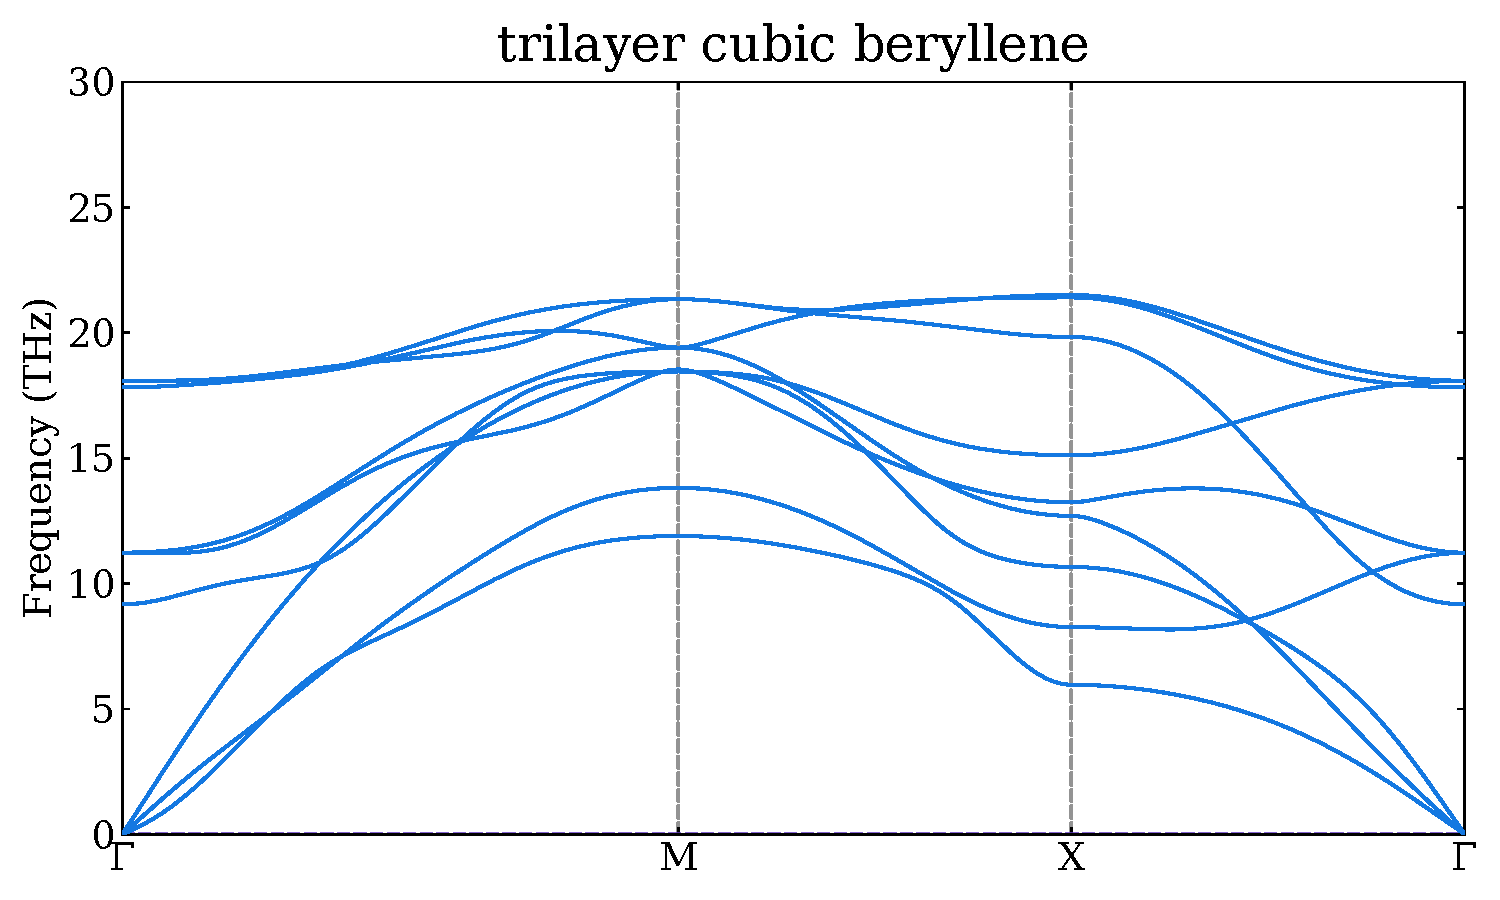
\includegraphics[width=0.40\linewidth]{figures_proj3/phonon_cubic-beryllene-trilayer_thesis.pdf}}%
    &\adjustbox{valign=c}{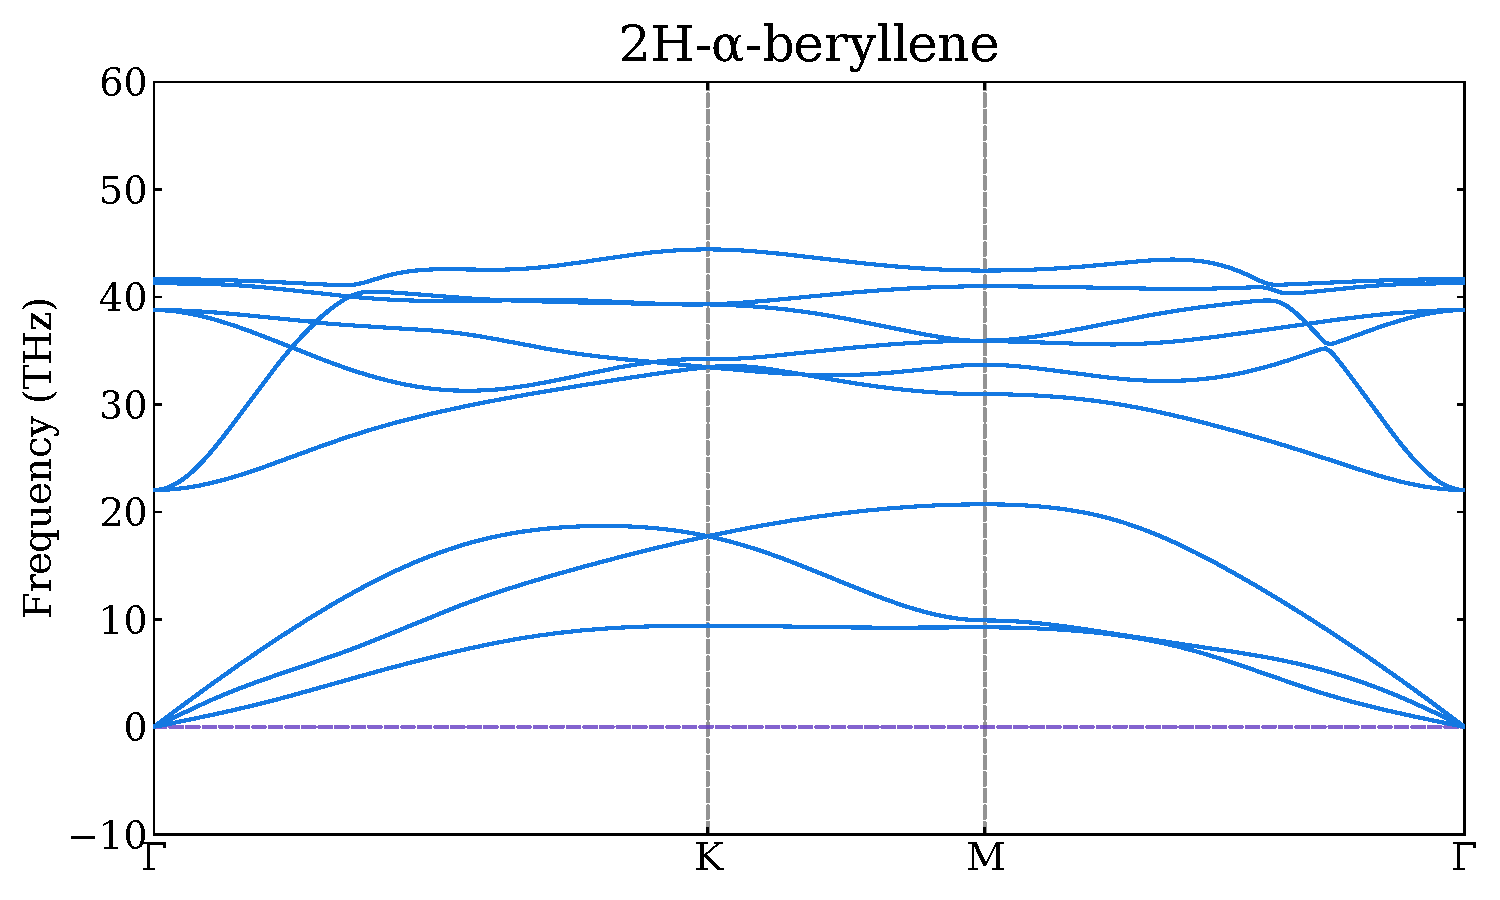
\includegraphics[width=0.40\linewidth]{figures_proj3/phonon_2H-alpha-beryllene_thesis.pdf}}%
    \\\adjustbox{valign=c}{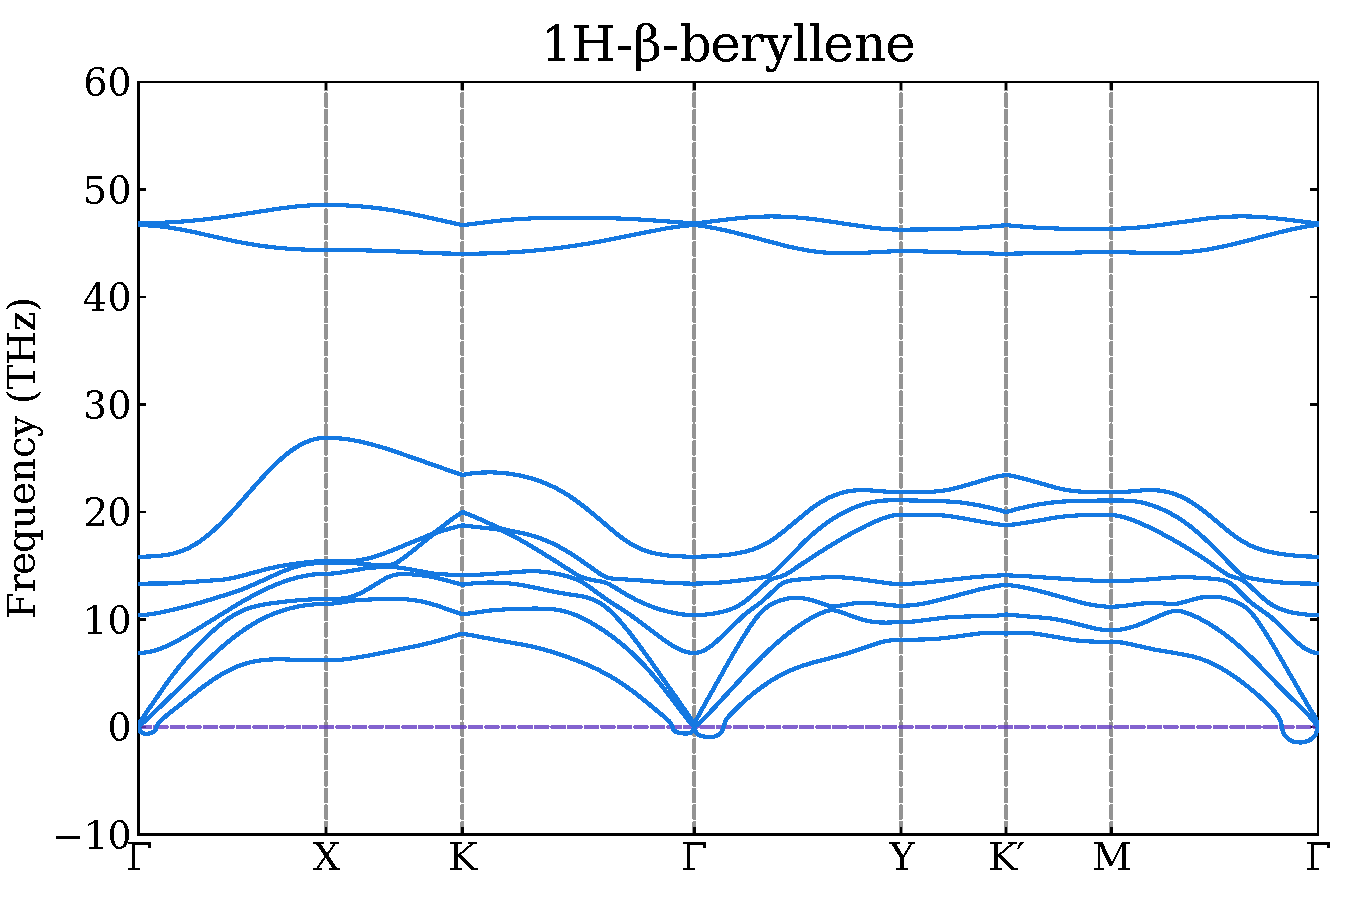
\includegraphics[width=0.40\linewidth]{figures_proj3/phonon_1H-beta-beryllene_thesis.pdf}}%
    &\adjustbox{valign=c}{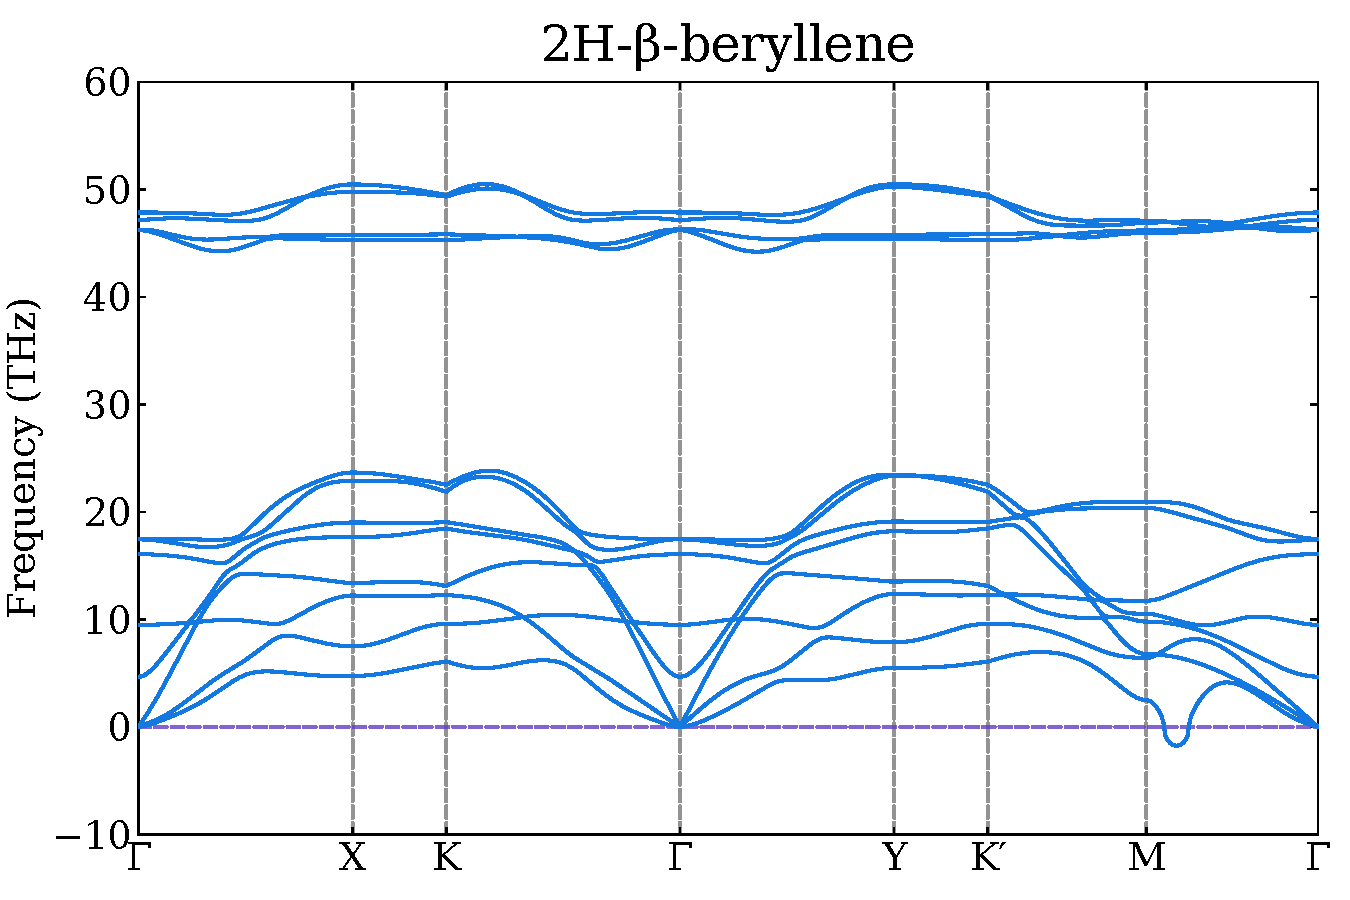
\includegraphics[width=0.40\linewidth]{figures_proj3/phonon_2H-beta-beryllene_thesis.pdf}}%
\end{tabular}
\caption{Phonon-dispersion curves of trilayer cubic beryllene and the hydrogen-functionalized beryllene structures.
Upper left: trilayer cubic beryllene. Upper right: 2H-$\alpha$-beryllene.
Lower left: 1H-$\beta$-beryllene. Lower right: 2H-$\beta$-beryllene.
Imaginary frequencies are shown as negative values.}
\label{fig:proj3_cubic_hydrogenated_phonons}
\end{figure}

We next follow the three hydrogen-functionalized structures at finite temperature using AIMD.
Figure~\ref{fig:proj3_hydrogenated_aimd} shows their energy and temperature trajectories and their final structures.
The total energy fluctuates around a steady mean, and the temperature fluctuates around \qty{300}{\kelvin}.
After \qty{5.5}{\pico\second}, each layer retains its Be framework and attached hydrogen.

\begin{figure}[!htbp]
\centering
\begin{tabular}{@{}c@{}c@{}}
    \adjustbox{valign=c}{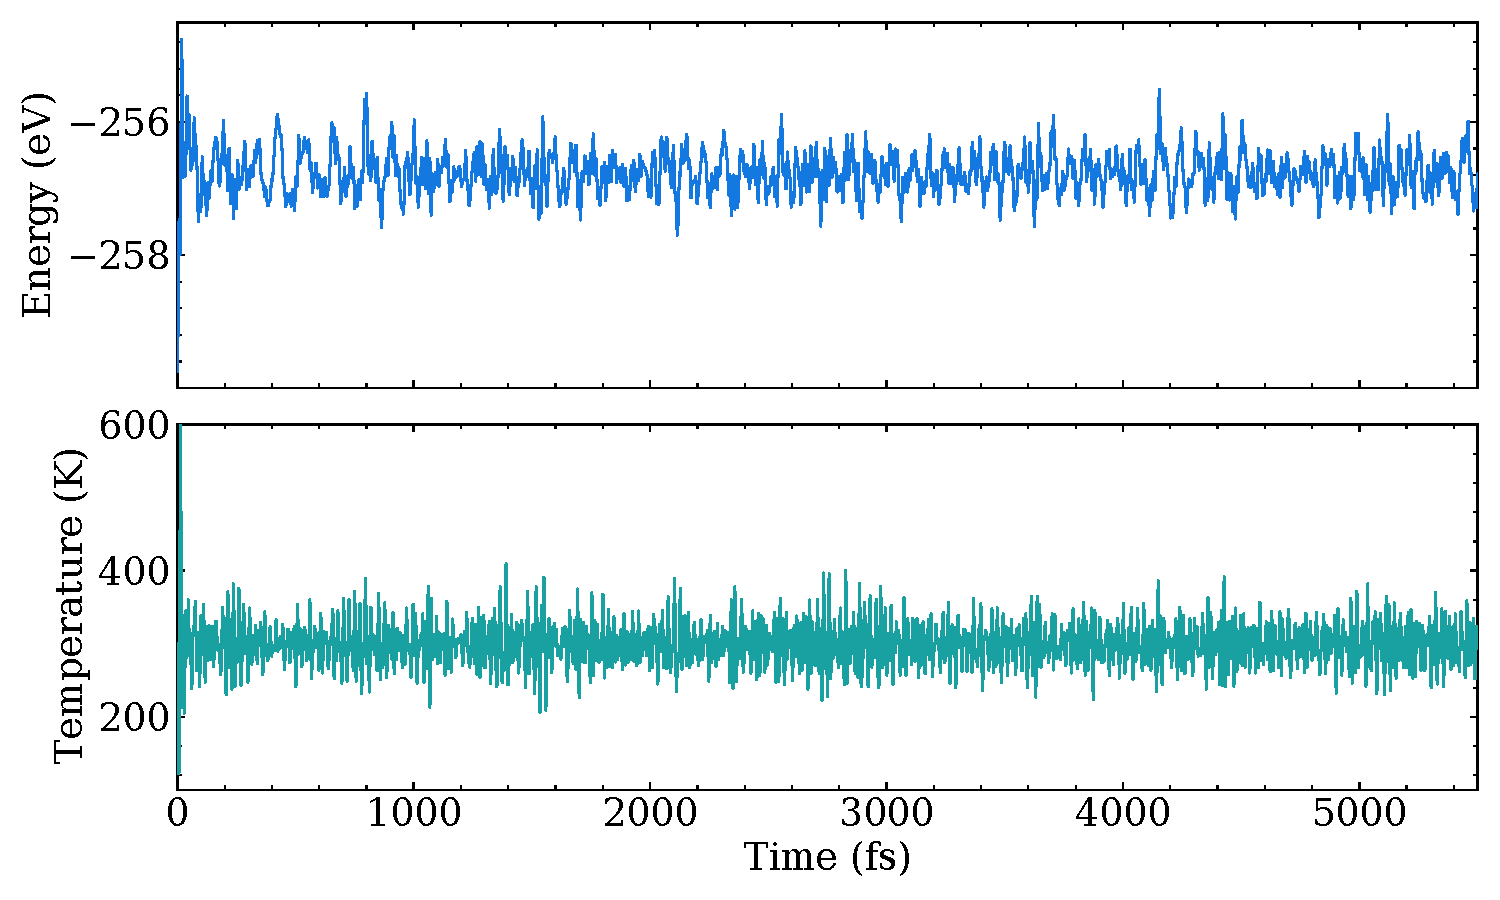
\includegraphics[width=0.50\linewidth]{figures_proj3/aimd_2H-alpha-beryllene_thesis.pdf}}%
    & \adjustbox{valign=c}{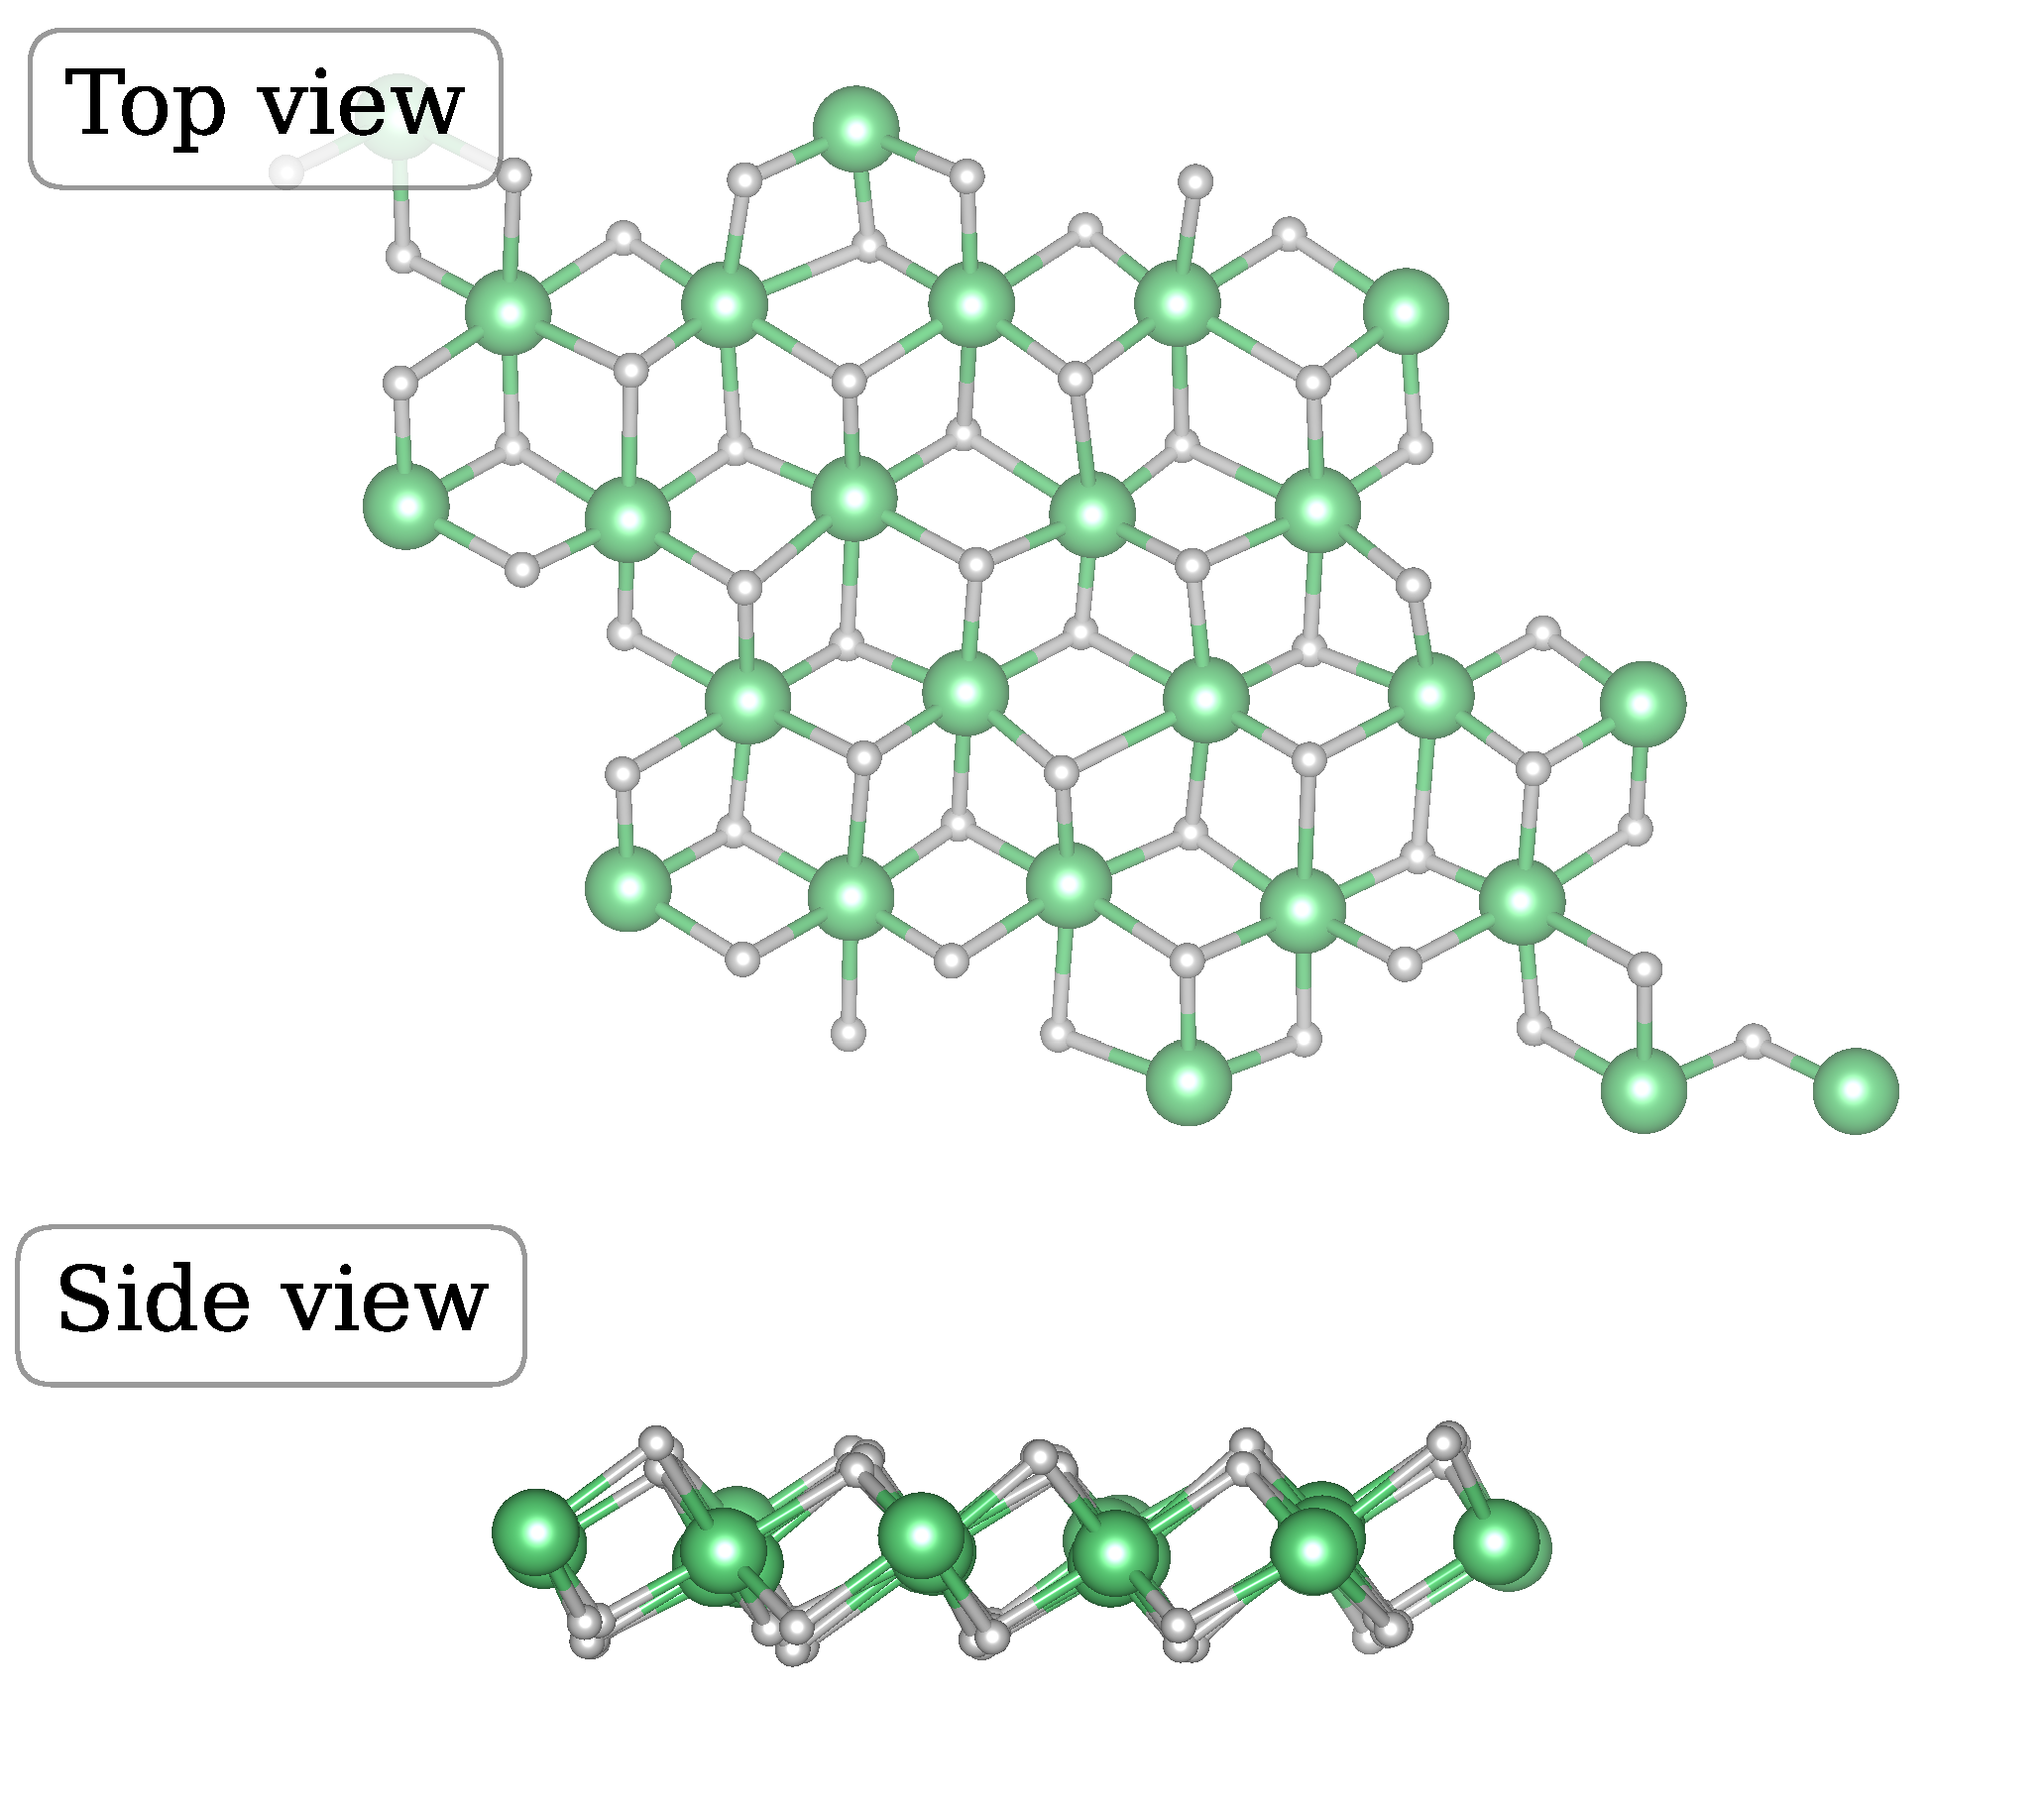
\includegraphics[width=0.30\linewidth]{figures_proj3/structure_2H-alpha-beryllene_thesis.pdf}}\\
    \adjustbox{valign=c}{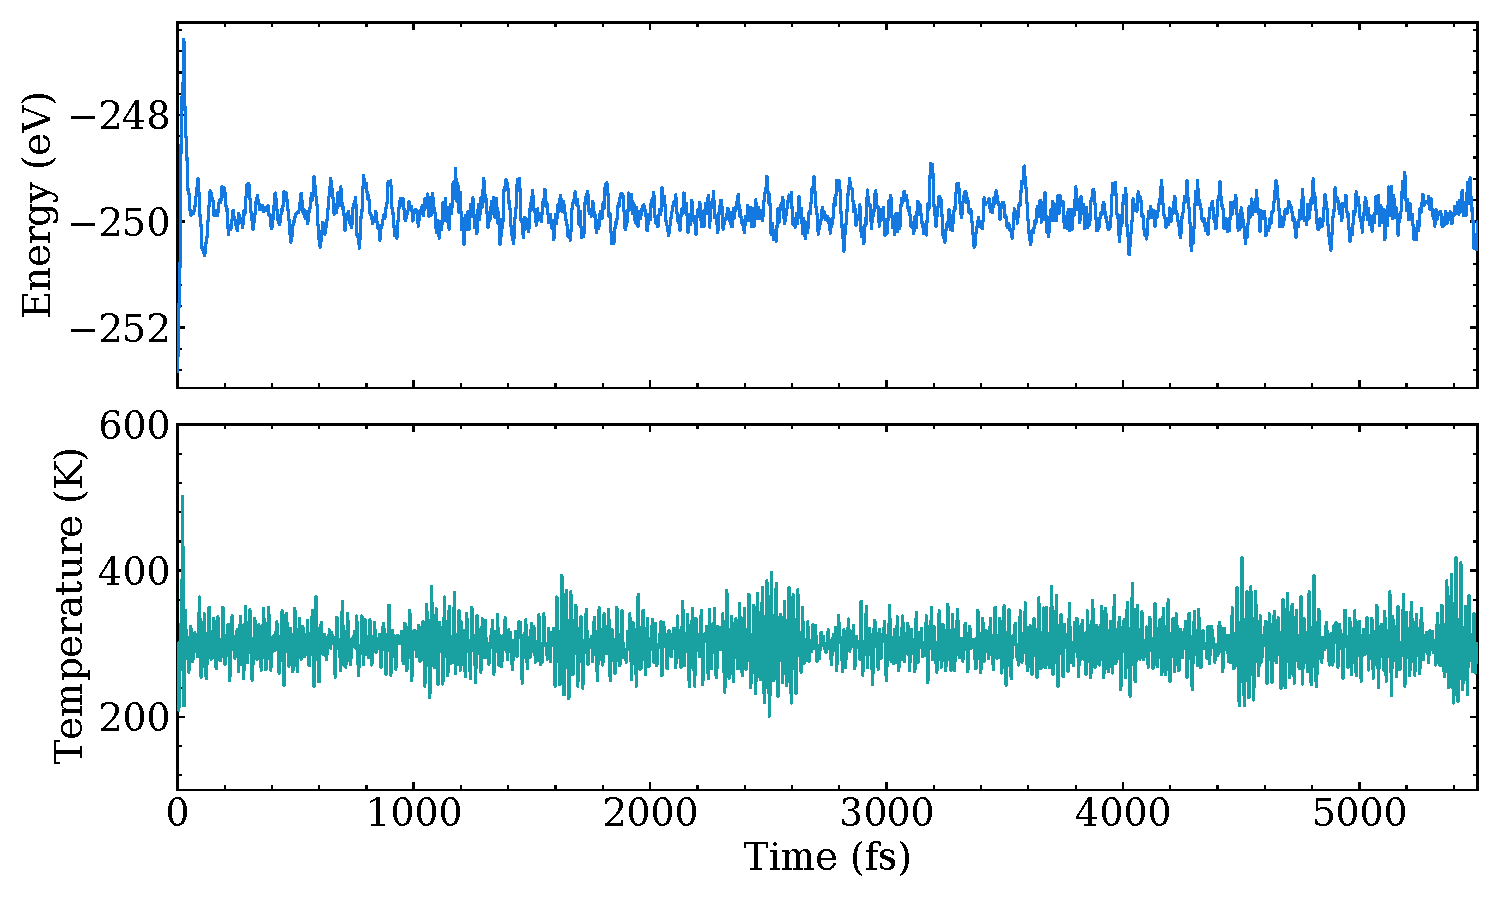
\includegraphics[width=0.50\linewidth]{figures_proj3/aimd_1H-beta-beryllene_thesis.pdf}}%
    & \adjustbox{valign=c}{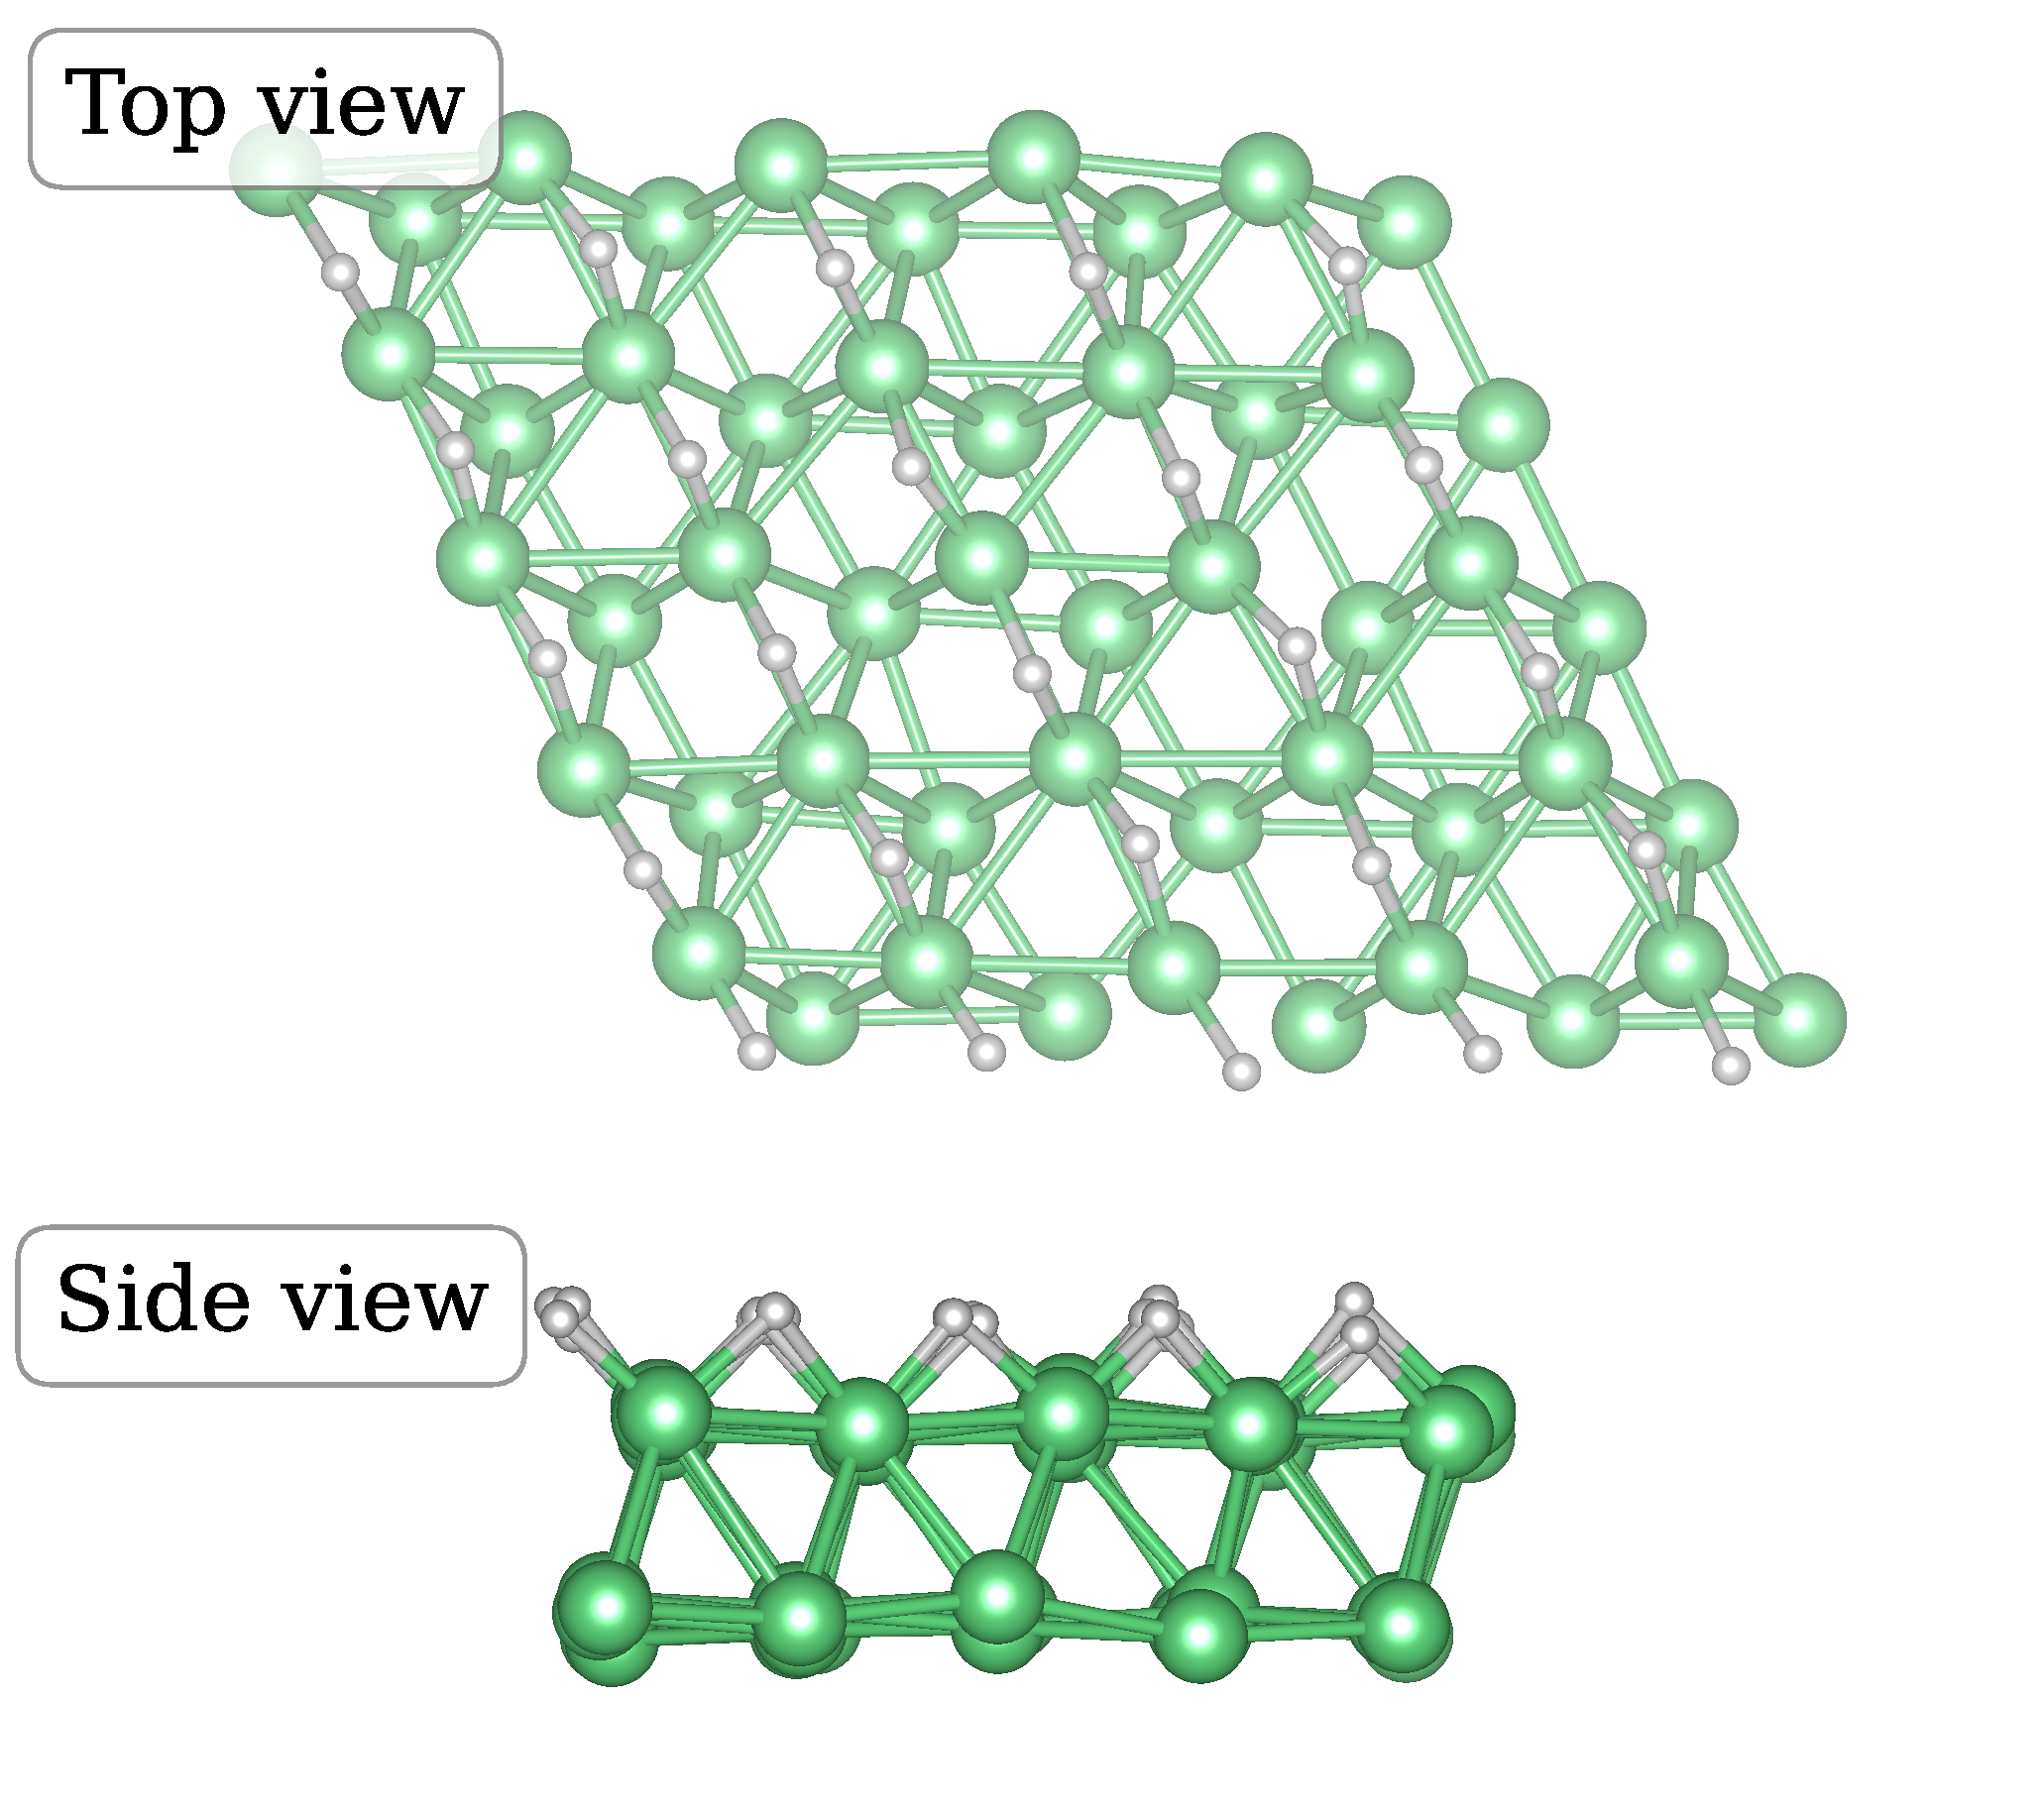
\includegraphics[width=0.30\linewidth]{figures_proj3/structure_1H-beta-beryllene_thesis.pdf}}\\
    \adjustbox{valign=c}{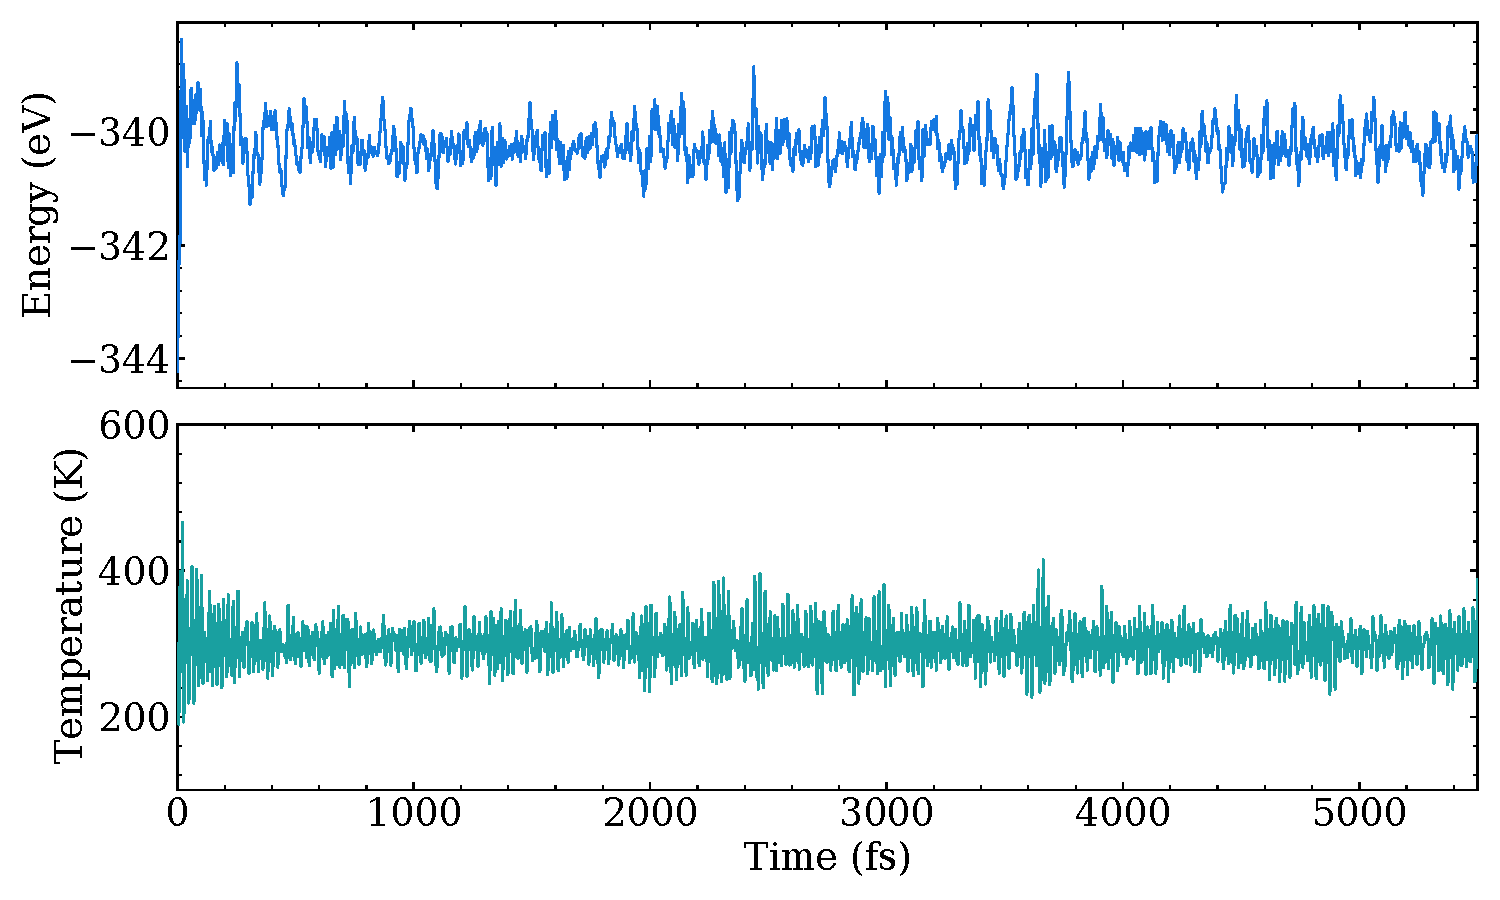
\includegraphics[width=0.50\linewidth]{figures_proj3/aimd_2H-beta-beryllene_thesis.pdf}}%
    & \adjustbox{valign=c}{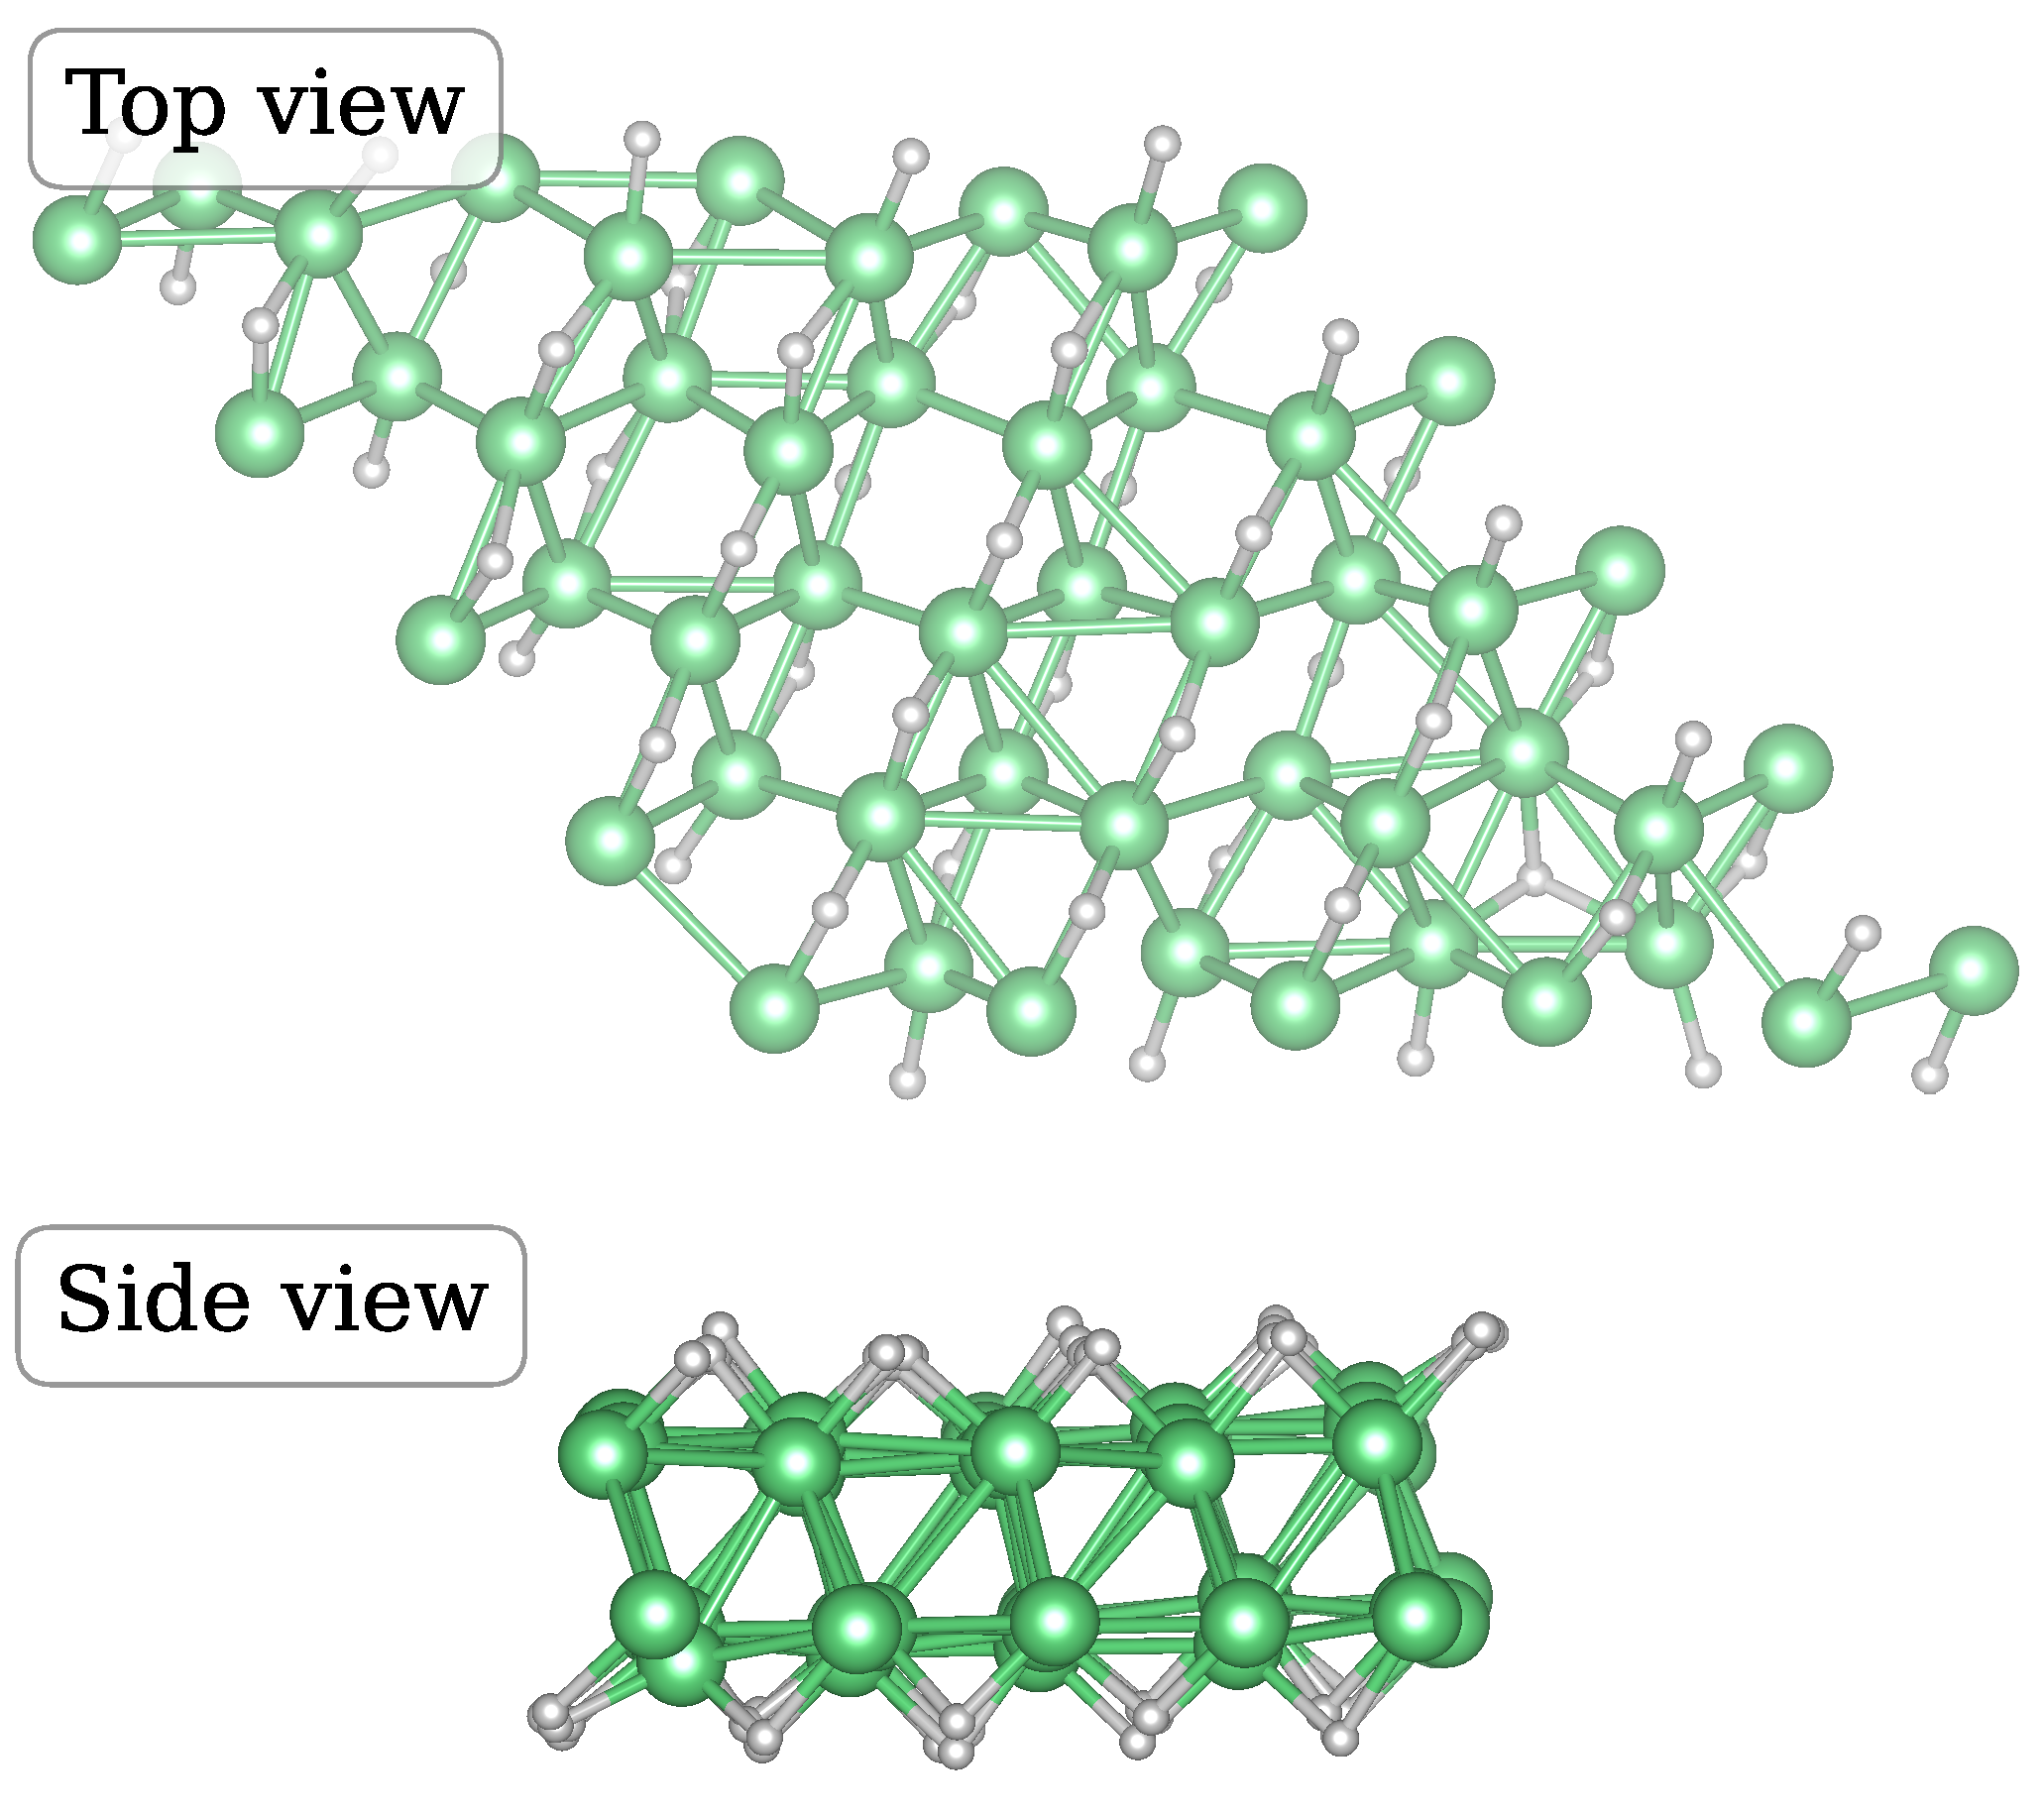
\includegraphics[width=0.30\linewidth]{figures_proj3/structure_2H-beta-beryllene_thesis.pdf}}
\end{tabular}
\caption{\textit{Ab initio} molecular dynamics simulations and corresponding atomic structures of the hydrogen-functionalized beryllene phases.
Upper: 2H-$\alpha$-beryllene.
Middle: 1H-$\beta$-beryllene.
Lower: 2H-$\beta$-beryllene.
For each row,
the left column shows the total energy and temperature as functions of simulation time,
and the right column shows the top and side views of the final structure at \qty{5.5}{\pico\second},
with beryllium in green and hydrogen in grey.}
\label{fig:proj3_hydrogenated_aimd}
\end{figure}

\subsection{Hydrogen adsorption energetics}
\label{3_hydrogen_adsorption_energetics}

Table~\ref{tab:proj3_hydrogenated_structural_parameters} gives the relaxed geometries and electronic adsorption energies.
Hydrogenation increases the in-plane lattice constant of $\alpha$-beryllene from \qty{2.129}{\angstrom} to \qty{2.322}{\angstrom}.
In 1H-$\beta$-beryllene, the in-plane lattice vectors have lengths of \qty{2.322}{\angstrom} and \qty{2.108}{\angstrom} and enclose an angle of \qty{117}{\degree}.
In 2H-$\beta$-beryllene, both lengths round to \qty{2.596}{\angstrom} and the angle increases to \qty{133}{\degree}.
Both hydrogenated $\beta$ structures therefore depart from the pristine hexagonal lattice.

The electronic adsorption energies relative to \ce{H2} are \qty{-0.33}{\electronvolt}, \qty{-0.07}{\electronvolt}, and \qty{-0.17}{\electronvolt} per hydrogen atom for 2H-$\alpha$-beryllene, 1H-$\beta$-beryllene, and 2H-$\beta$-beryllene, respectively.
Zero-point motion raises all three adsorption energies and changes the sign for 1H-$\beta$-beryllene, from \qty{-0.07}{\electronvolt} to \qty{0.01}{\electronvolt} per hydrogen atom.
At \qty{298.15}{\kelvin} and a \ce{H2} pressure of \qty{1}{\bar}, the corresponding adsorption free energies are \qty{-0.08}{\electronvolt}, \qty{0.17}{\electronvolt}, and \qty{0.06}{\electronvolt} per hydrogen atom.
Only 2H-$\alpha$-beryllene therefore favours adsorption from the gas under these conditions.
A barrier to hydrogen release could nevertheless allow the hydrogenated $\beta$ phases to persist.
For 2H-$\beta$-beryllene, the estimated equilibrium \ce{H2} pressure at \qty{298.15}{\kelvin} is about \qty{90}{\bar} in the harmonic treatment with the imaginary modes omitted.
Table~\ref{tab:proj3_hydrogenation_energetics} gives the energy and pressure estimates.

Since 2H-$\alpha$-beryllene has the composition \ce{BeH2}, we also compare its electronic energy with those of two square \ce{BeH2} monolayers relaxed with the same settings.
In the puckered square structure, four bridging hydrogen atoms surround each Be atom in tetrahedral coordination at \qty{1.468}{\angstrom}, as in bulk \ce{BeH2}.
This structure lies \qty{38}{\milli\electronvolt} per formula unit below 2H-$\alpha$-beryllene in electronic energy.
The planar square layer lies \qty{1.23}{\electronvolt} per formula unit above it.
Conversion from 2H-$\alpha$-beryllene to the puckered layer requires a rearrangement from a triangular to a square Be lattice.
The comparison in table~\ref{tab:proj3_beh2_polymorphs} ranks the relaxed structures tested.
The dynamical stability of the puckered layer and the barrier for reconstruction remain open.

\begin{table}[!htbp]
\centering
\rowcolors{2}{gray!15}{white}
\begin{adjustbox}{max width=1.0\linewidth,center}
\begin{tabular}{cccccccc}
\hline
\rowcolor{gray!25}
system
& $a$
& $b$
& Be layer spacing (\AA)
& Be-H (\AA)
& $E_{\mathrm{ad}}$ (eV)
& angle
& electronic nature \\
\hline
2H-$\alpha$-beryllene
& 2.322 & 2.322 & -- & 1.599 & $-0.33$ & $120^{\circ}$ & semiconductor \\
1H-$\beta$-beryllene
& 2.322 & 2.108 & 1.849 & 1.451 & $-0.07$ & $117^{\circ}$ & metallic \\
2H-$\beta$-beryllene
& 2.596 & 2.596 & 1.786 & 1.446 & $-0.17$ & $133^{\circ}$ & metallic \\
\hline
\end{tabular}
\end{adjustbox}
\caption{Relaxed lattice constants $a$ and $b$, Be layer spacing, Be-H bond length, and in-plane lattice angle for the hydrogen-functionalized beryllene structures.
All lengths are in \unit{\angstrom}.
The electronic adsorption energy $E_{\mathrm{ad}}$ is given per hydrogen atom relative to the pristine layer and \ce{H2}.}
\label{tab:proj3_hydrogenated_structural_parameters}
\end{table}

\subsection{Electronic properties}
\label{3_electronic_properties}

We now compare the electronic bands of the pristine and hydrogen-functionalized phases.
The $\alpha$- and $\beta$-beryllene bands in figure~\ref{fig:proj3_band_structures} agree with previous calculations~\cite{li2023coexistence}.
Figure~\ref{fig:proj3_band_structures_cubic_hydrogenated} shows several bands crossing the Fermi level in the cubic trilayer, establishing its metallic character within PBE.
Band splittings near $\Gamma$, $\mathrm{M}$, and $\mathrm{X}$ are consistent with coupling between the three layers.

Hydrogenation opens an indirect gap of \qty{4.84}{\electronvolt} in 2H-$\alpha$-beryllene at the PBE level.
With both PBE and HSE06, the sampled valence-band maximum lies on $\Gamma$--$\mathrm{K}$ and the conduction-band minimum on $\Gamma$--$\mathrm{M}$.
HSE06 increases the indirect gap to \qty{6.00}{\electronvolt}.
Its smallest sampled direct gap, between states at the same wave vector, is \qty{6.09}{\electronvolt}.
Both hydrogenated $\beta$ phases retain bands crossing the Fermi level and therefore remain metallic.

\begin{figure}[!htbp]
\centering
\begin{tabular}{@{}cc@{}}
    \adjustbox{valign=c}{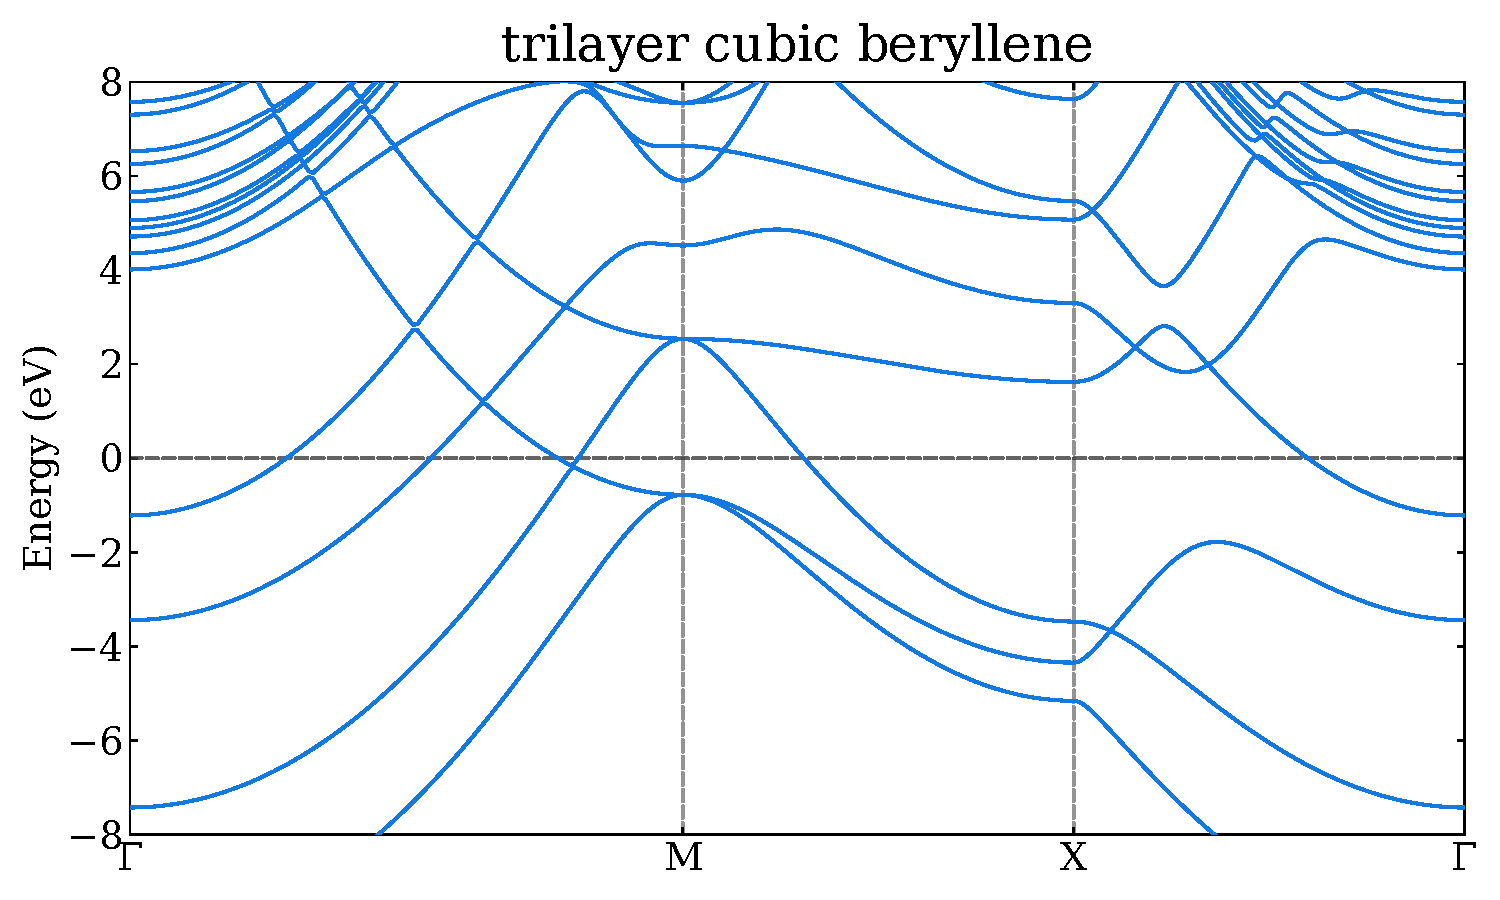
\includegraphics[width=0.40\linewidth]{figures_proj3/bands_cubic-beryllene-trilayer_thesis.pdf}}&
    \adjustbox{valign=c}{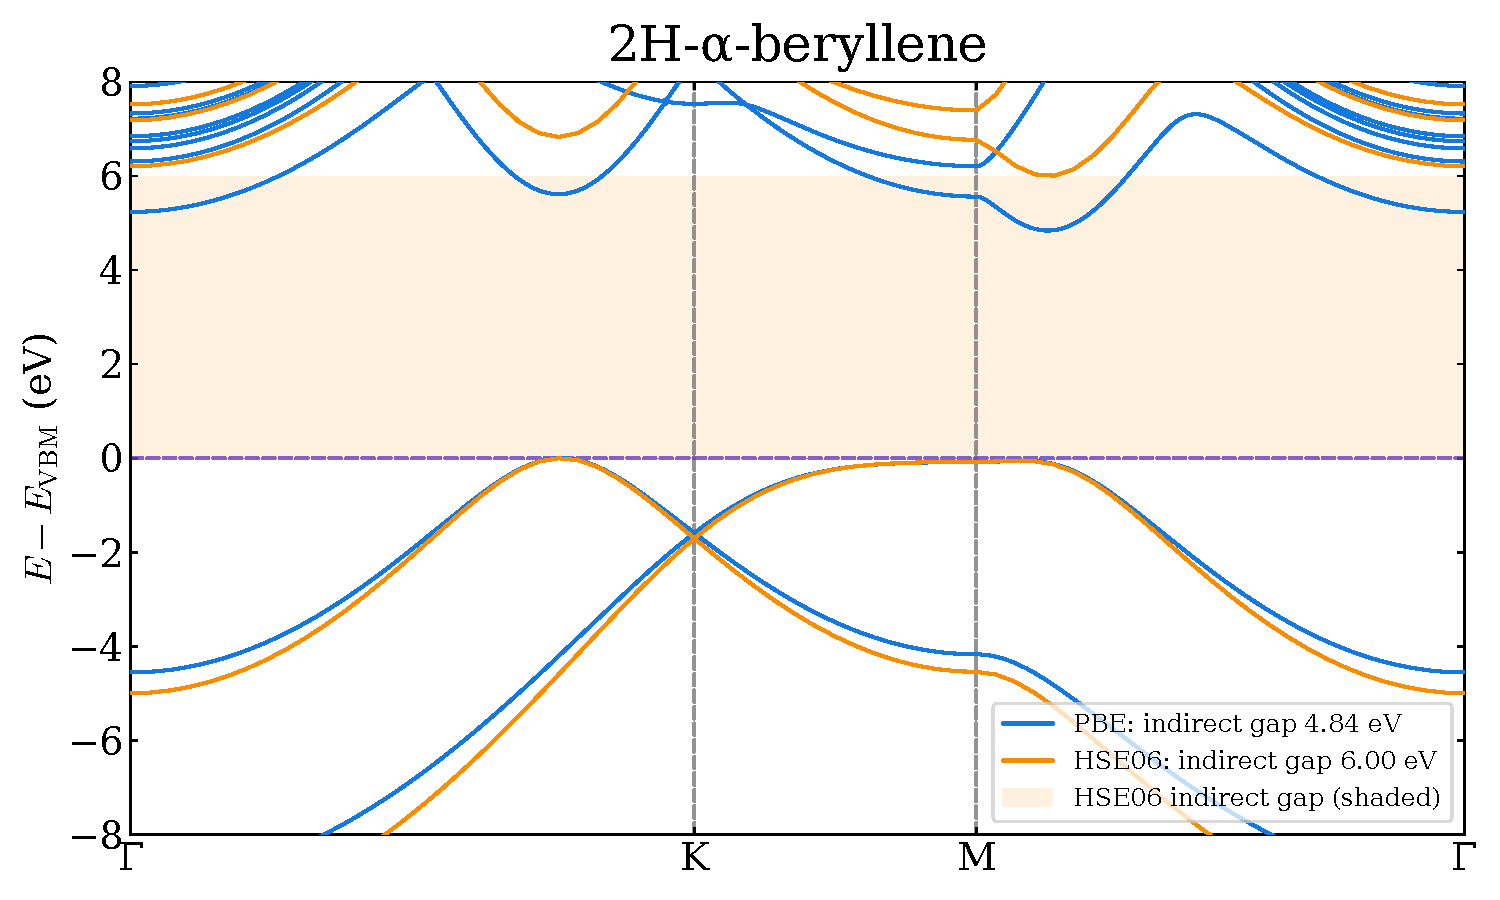
\includegraphics[width=0.40\linewidth]{figures_proj3/bands_2H-alpha-beryllene_thesis.pdf}}\\
    \adjustbox{valign=c}{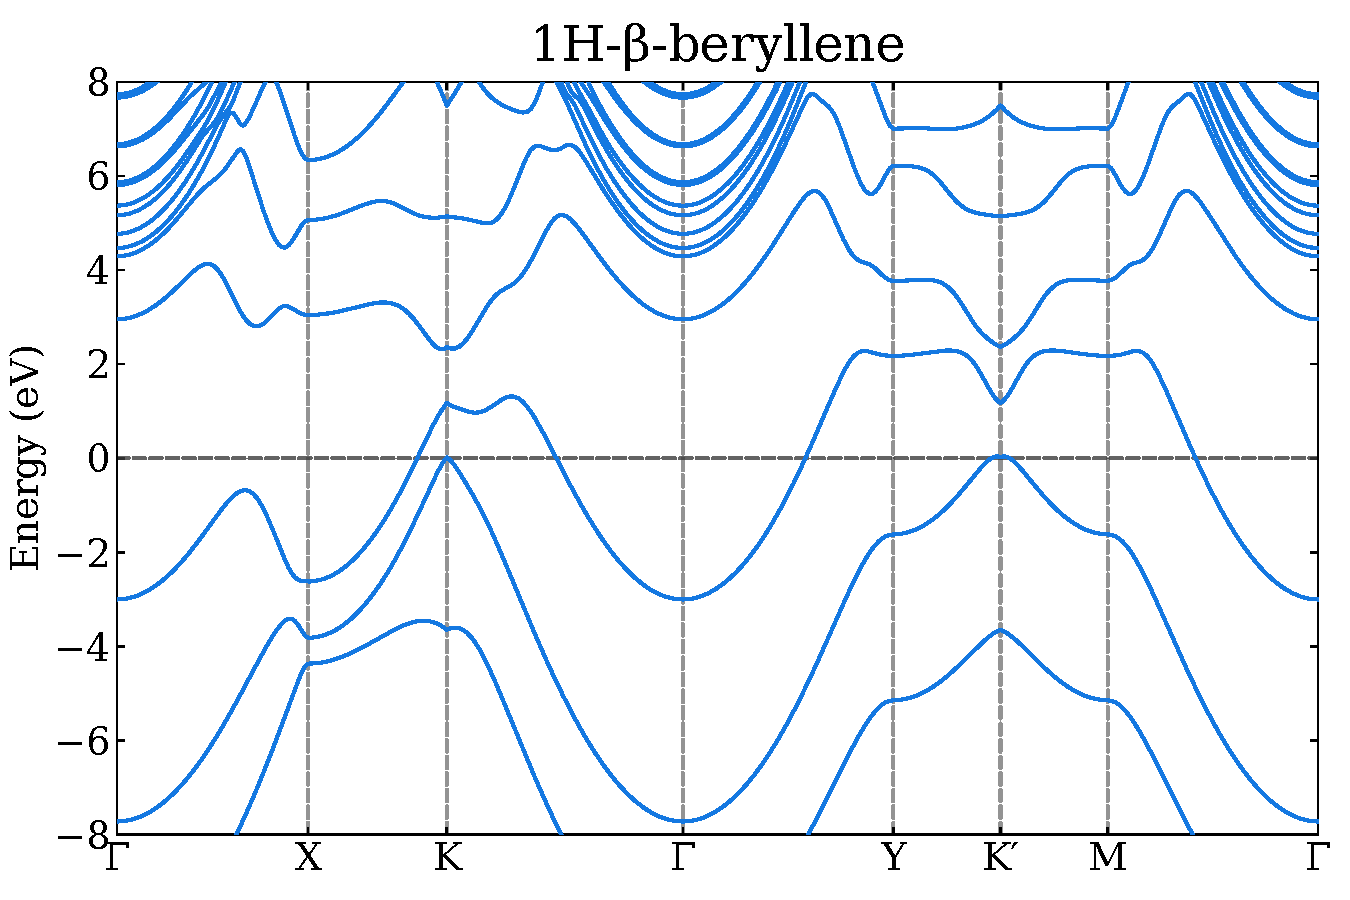
\includegraphics[width=0.40\linewidth]{figures_proj3/bands_1H-beta-beryllene_thesis.pdf}}&
    \adjustbox{valign=c}{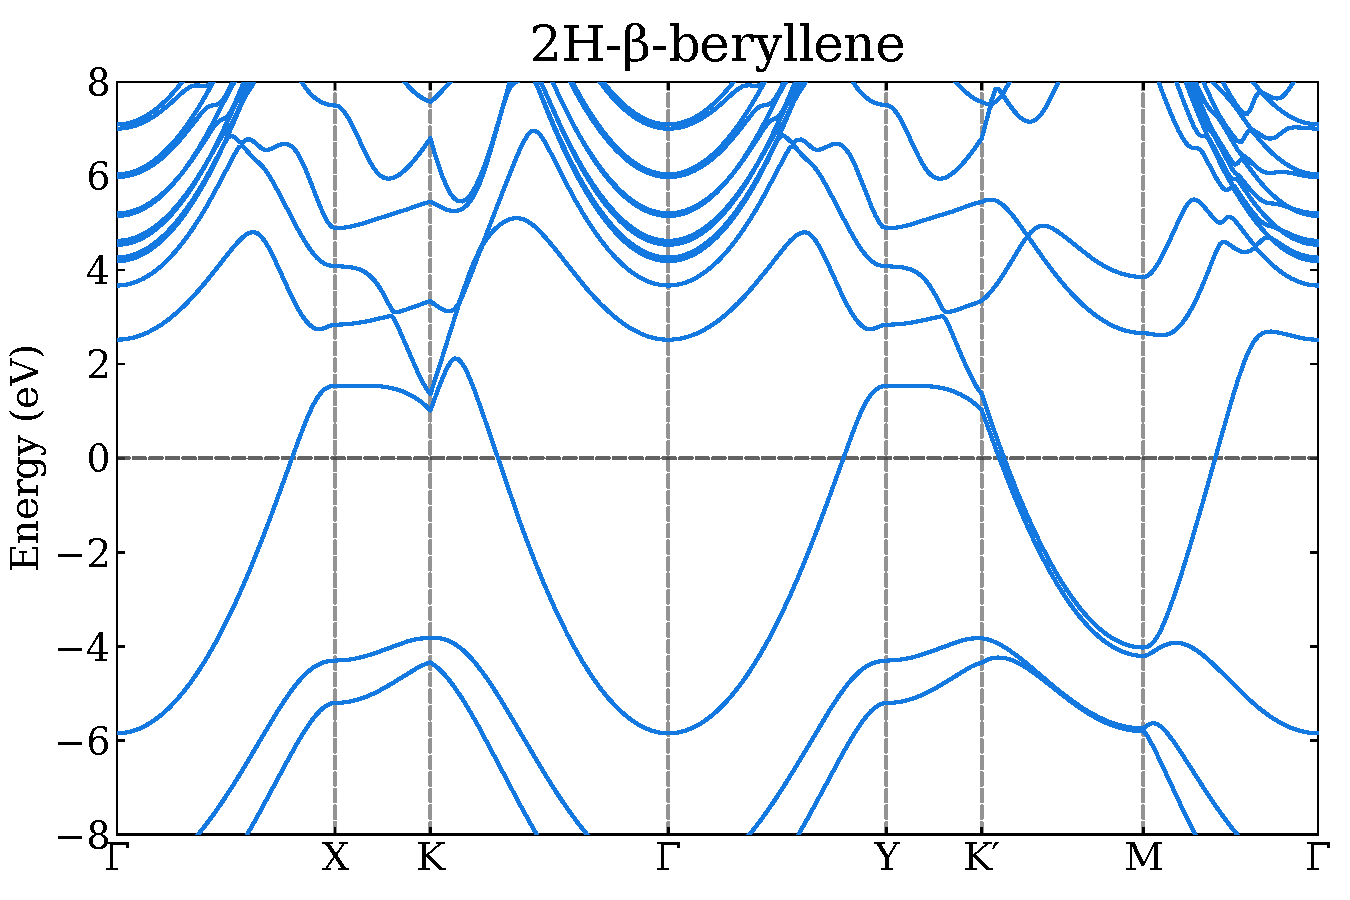
\includegraphics[width=0.40\linewidth]{figures_proj3/bands_2H-beta-beryllene_thesis.pdf}}
\end{tabular}
\caption{Band structures of trilayer cubic beryllene and the hydrogen-functionalized beryllene structures.
Upper left: trilayer cubic beryllene. Upper right: 2H-$\alpha$-beryllene.
Lower left: 1H-$\beta$-beryllene. Lower right: 2H-$\beta$-beryllene.
For 1H-$\beta$-beryllene and 2H-$\beta$-beryllene,
the path $\Gamma$--$\mathrm{X}$--$\mathrm{K}$--$\Gamma$--$\mathrm{Y}$--$\mathrm{K}'$--$\mathrm{M}$--$\Gamma$ passes through all four time-reversal invariant momenta and the zone corners $\mathrm{K}$ and $\mathrm{K}'$,
as for the phonon dispersions in figure~\ref{fig:proj3_cubic_hydrogenated_phonons}.
For 2H-$\alpha$-beryllene,
the PBE (blue) and HSE06 (orange) bands are each aligned at their valence-band maximum.}
\label{fig:proj3_band_structures_cubic_hydrogenated}
\end{figure}

Figure~\ref{fig:proj3_dos_cubic_trilayer} compares the total density of states of bulk bcc beryllium and the cubic trilayer.
The trilayer has a finite density of states at the Fermi level, consistent with the band crossings.

\begin{figure}[!htbp]
\centering
    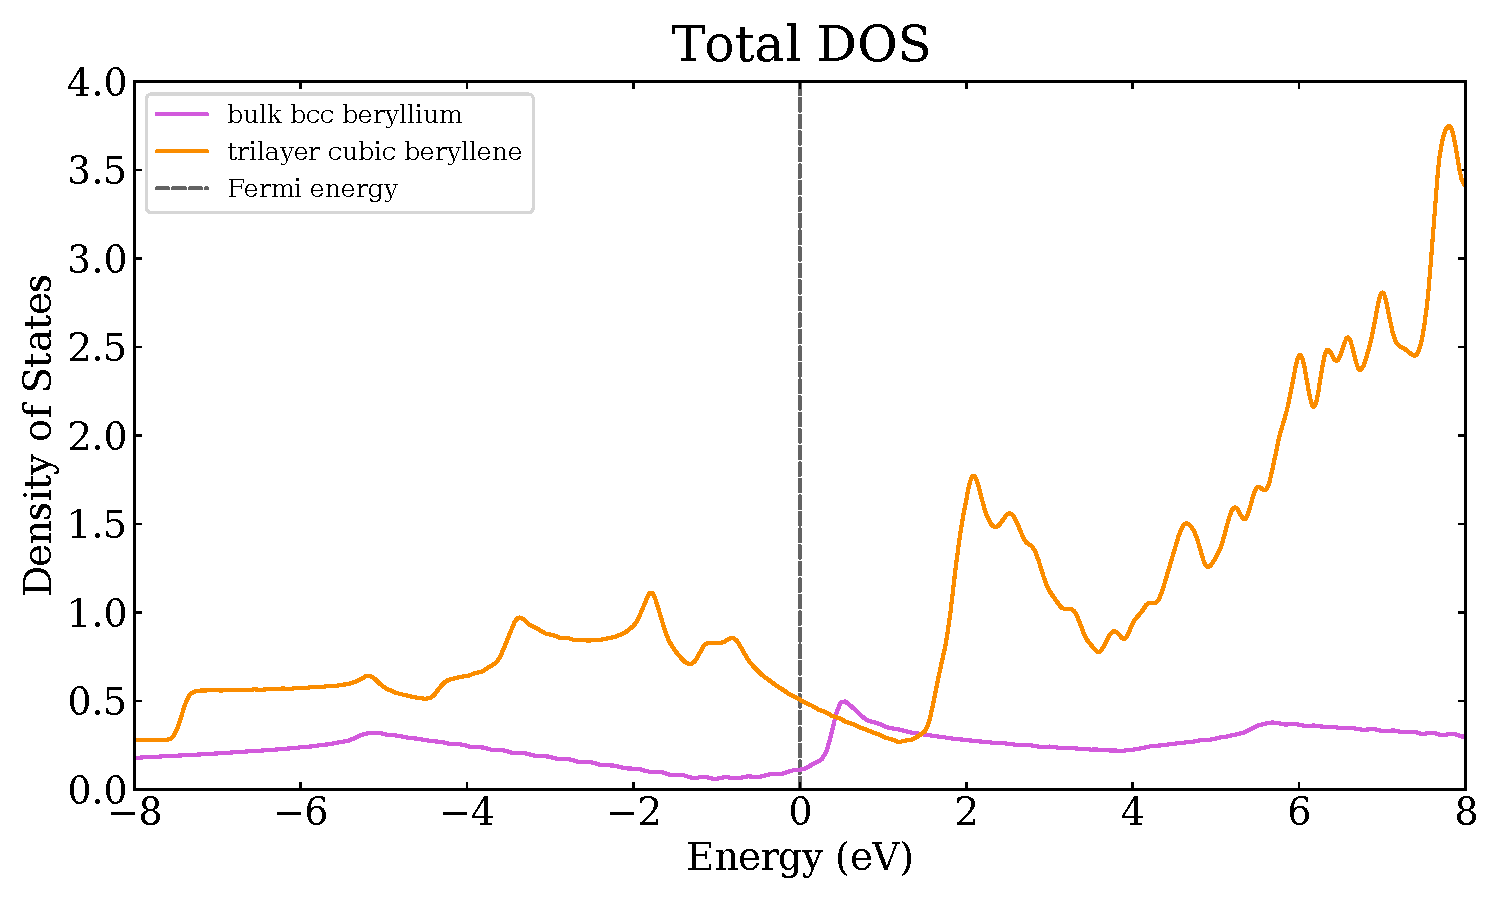
\includegraphics[width=0.6\linewidth]{figures_proj3/dos_cubic-family_thesis.pdf}
\caption{Total density of states of bulk bcc beryllium and trilayer cubic beryllene.}
\label{fig:proj3_dos_cubic_trilayer}
\end{figure}

Figure~\ref{fig:proj3_dos_hydrogenated} compares the densities of states of the pristine and hydrogen-functionalized phases.
The total density of states vanishes around the Fermi level in 2H-$\alpha$-beryllene and remains finite in both hydrogenated $\beta$ phases.
The projected densities of states show Be $s$ and $p$ and H $1s$ weight over common energy ranges, consistent with Be-H hybridization.
At this stage, we arrive at the metallic and semiconducting cases for the topology analysis below.

\begin{figure}[!htbp]
\centering
\begin{tabular}{@{}cc@{}}
    \adjustbox{valign=c}{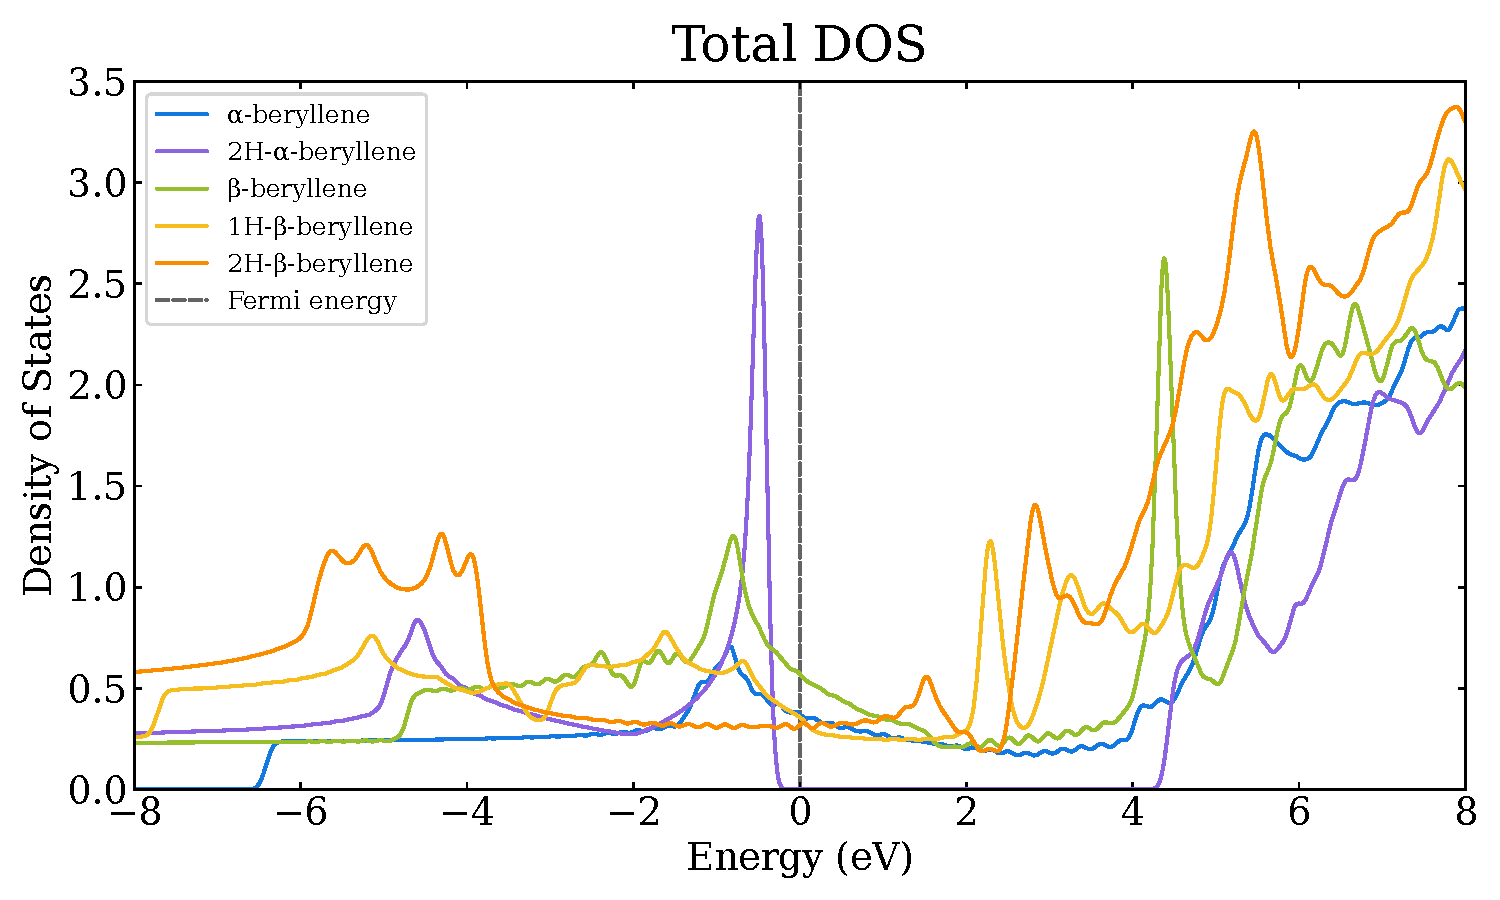
\includegraphics[width=0.40\linewidth]{figures_proj3/dos_hydrogenated_thesis.pdf}}&
    \adjustbox{valign=c}{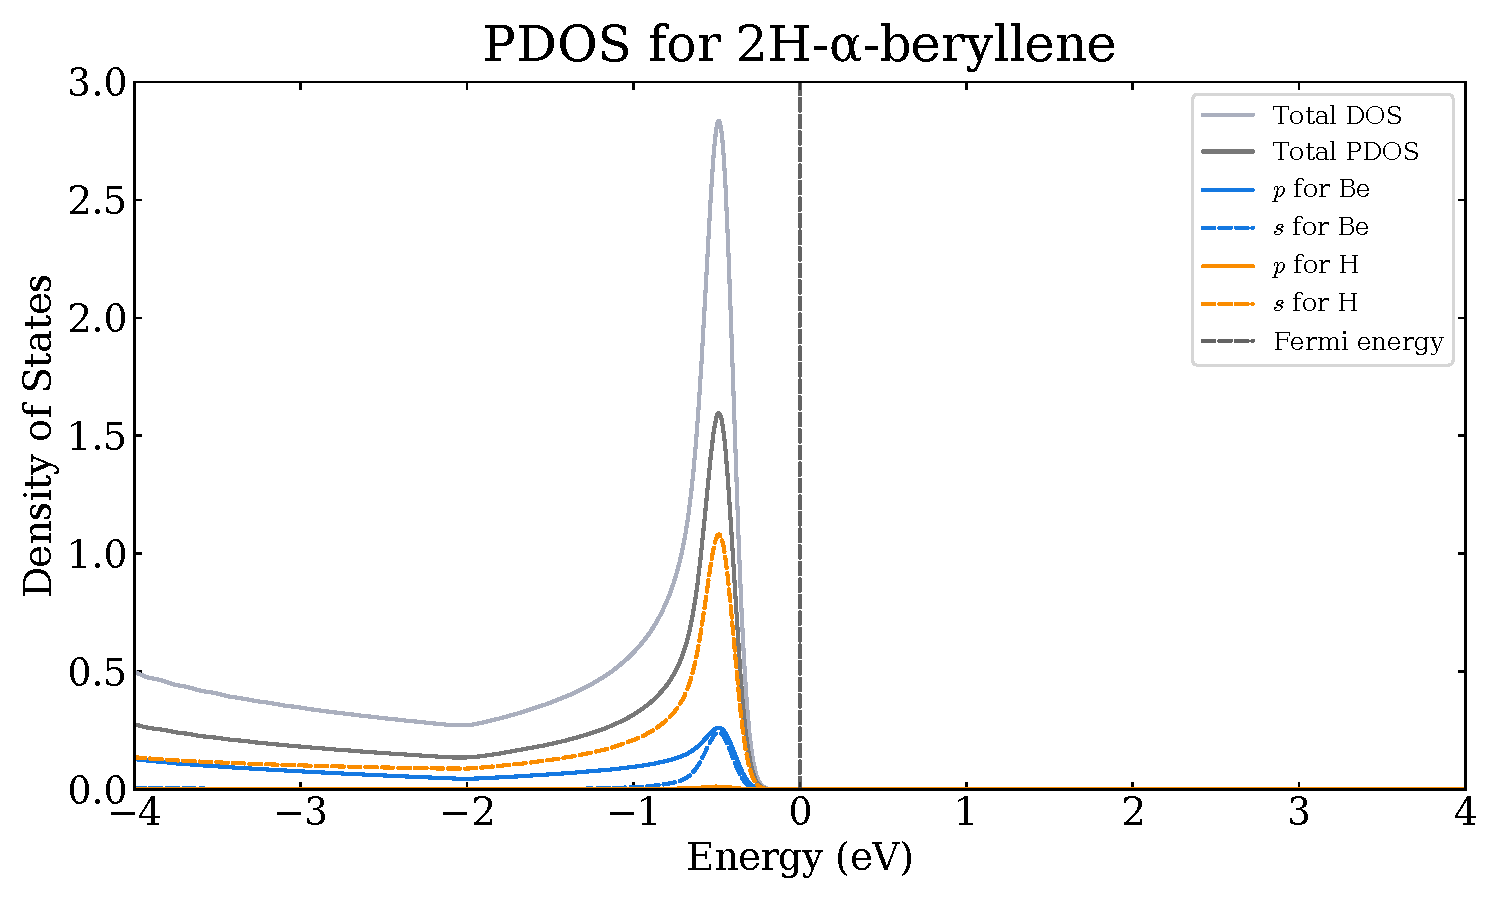
\includegraphics[width=0.40\linewidth]{figures_proj3/pdos_2H-alpha-beryllene_thesis.pdf}}\\
    \adjustbox{valign=c}{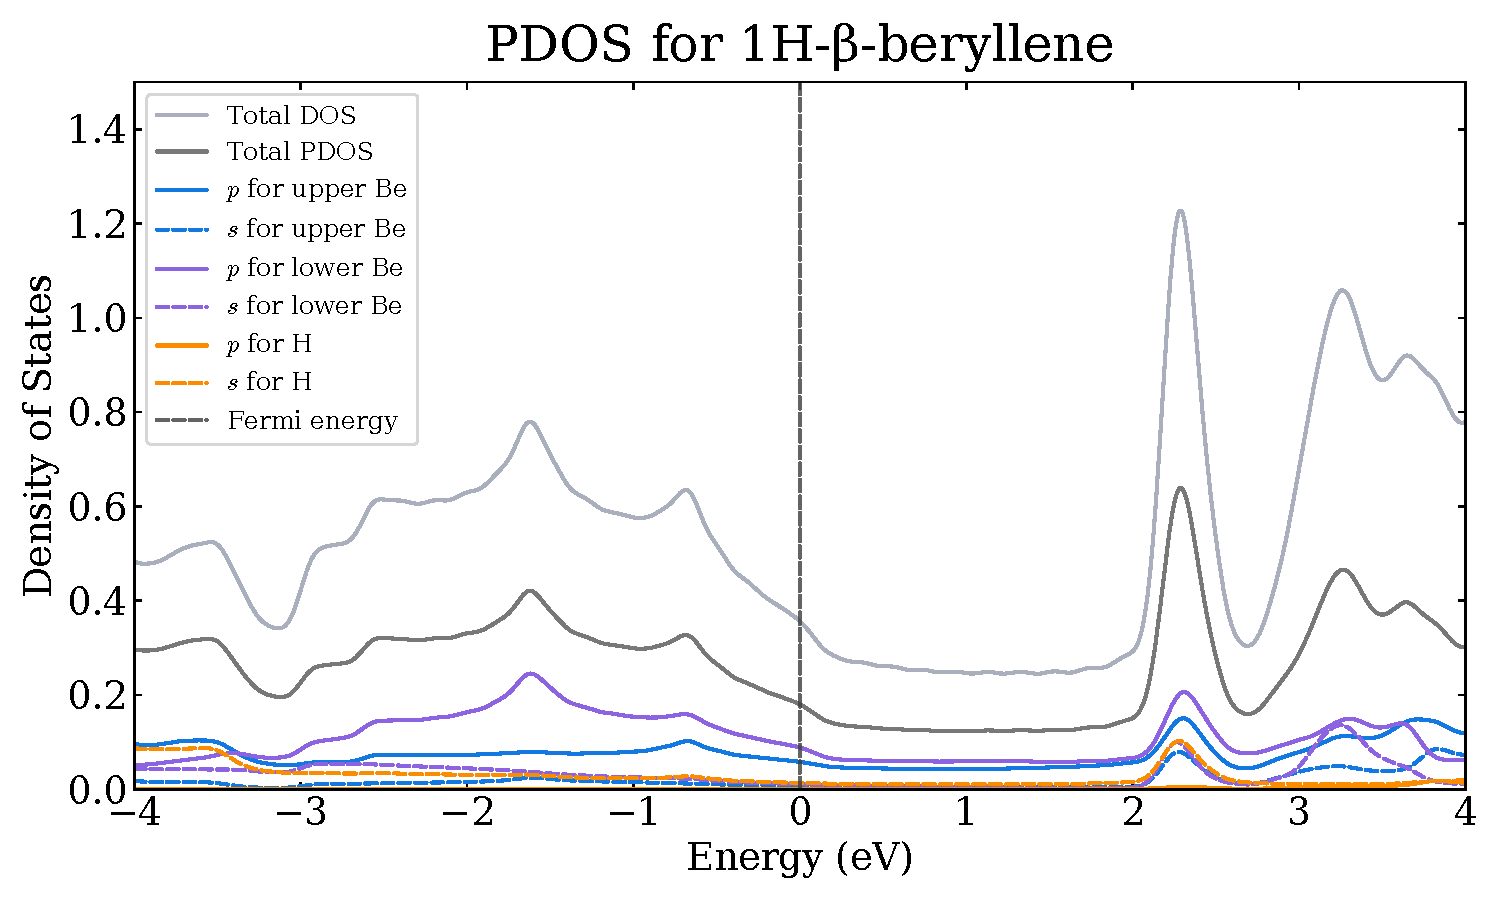
\includegraphics[width=0.40\linewidth]{figures_proj3/pdos_1H-beta-beryllene_thesis.pdf}}&
    \adjustbox{valign=c}{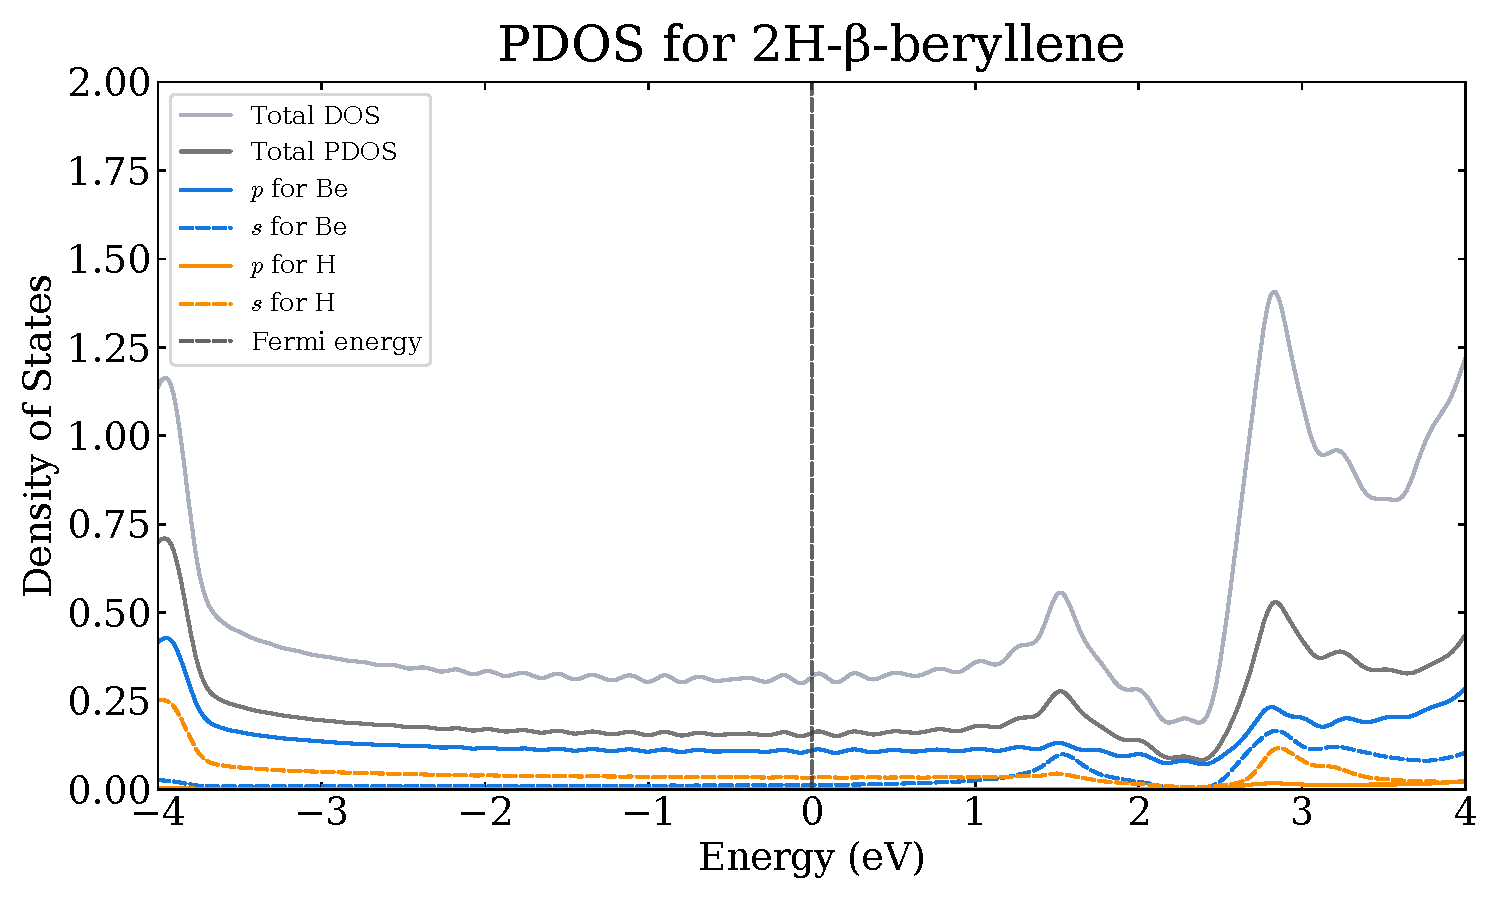
\includegraphics[width=0.40\linewidth]{figures_proj3/pdos_2H-beta-beryllene_thesis.pdf}}
\end{tabular}
\caption{Total and projected densities of states for pristine and hydrogen-functionalized beryllene structures.
Upper left: total density of states.
Upper right: projected density of states of 2H-$\alpha$-beryllene.
Lower left: projected density of states of 1H-$\beta$-beryllene.
Lower right: projected density of states of 2H-$\beta$-beryllene.}
\label{fig:proj3_dos_hydrogenated}
\end{figure}

\subsection{Topological properties}
\label{3_topological_properties}

The band structures show that five of the six layers are metallic at neutral filling.
We now examine the topology of selected groups of bands in these layers and of the occupied bands in insulating 2H-$\alpha$-beryllene.
Previous calculations found a non-trivial index for $\alpha$-beryllene and a trivial index for $\beta$-beryllene~\cite{li2023coexistence}.

We apply the Fu--Kane criterion to the five structures with inversion symmetry.
The $\mathbb{Z}_2$ index $\nu$ follows from the parity products $\delta_i$ of the lowest $N$ spinor bands at the four time-reversal invariant momenta, according to equations~\eqref{eq:proj3_parity_product} and~\eqref{eq:proj3_z2_index}.
For 1H-$\beta$-beryllene, we obtain $\nu$ from the evolution of the Wannier charge centres, as described in section~\ref{3_methods}.

In a metal, the number of bands below the Fermi level varies with wave vector.
We instead follow the lowest $N$ bands at every $\vec{k}$, including them where they rise above the Fermi level.
The index characterizes this subspace when time-reversal symmetry holds and the direct gap $E_{N+1}(\vec{k}\,)-E_N(\vec{k}\,)$ remains positive throughout the Brillouin zone.
We use the smallest sampled direct gap to test this condition.
The finite mesh provides a screening result, conditional on isolation between the sampled points.

Table~\ref{tab:proj3_topological_parity} lists the parities, indices, and sampled gap minima.
For $\alpha$-beryllene, $\beta$-beryllene, and 2H-$\alpha$-beryllene, the three zone-boundary momenta are symmetry-equivalent $\mathrm{M}$ points of the hexagonal Brillouin zone.
Their Fu--Kane product therefore reduces to $(-1)^\nu=\delta_\Gamma\delta_\mathrm{M}$, since $(\delta_\mathrm{M})^3=\delta_\mathrm{M}$.
The same reduction holds for trilayer cubic beryllene because the two equivalent $\mathrm{X}$ points of the square Brillouin zone give a factor of $(\delta_\mathrm{X})^2=1$.
For the monoclinic 2H-$\beta$-beryllene, we use the parity products at all four momenta.

\begin{table}[!htbp]
\centering
\rowcolors{2}{gray!15}{white}
\setlength{\tabcolsep}{8pt}
\begin{adjustbox}{max width=1.0\linewidth,center}
\begin{tabular}{ccccccccc}
\hline
\rowcolor{gray!25}
structure
& $N$
& $\Gamma$
& $\mathrm{X}$
& $\mathrm{Y}$
& $\mathrm{M}$
& product
& $\nu$
& min. direct gap \\
\hline
$\alpha$-beryllene
& 2
& $+$
& $-$
& $-$
& $-$
& $-1$
& 1
& \qty{1.13}{\milli\electronvolt} \\
$\beta$-beryllene
& 4
& $+, -$
& $+, -$
& $+, -$
& $+, -$
& $+1$
& 0
& \qty{0.898}{\milli\electronvolt} \\
trilayer cubic beryllene
& 6
& $+, -, +$
& $+, -, +$
& $+, -, +$
& $-, -, +$
& $-1$
& 1
& \qty{0.735}{\milli\electronvolt} \\
2H-$\alpha$-beryllene
& 4
& $+, -$
& $-, +$
& $-, +$
& $-, +$
& $+1$
& 0
& \qty{4.92}{\electronvolt} \\
2H-$\beta$-beryllene
& 6
& $+, -, +$
& $-, +, +$
& $+, -, -$
& $-, +, -$
& $+1$
& 0
& \qty{0.177}{\electronvolt} \\
1H-$\beta$-beryllene
& 4 / 6
& --
& --
& --
& --
& --
& 0 / 0
& $(0.929,\,0.415)$~\unit{\electronvolt} \\
\hline
\end{tabular}
\end{adjustbox}
\caption{Parity eigenvalues of the Kramers pairs of the lowest $N$ spinor bands, ordered by increasing energy at each time-reversal invariant momentum.
The table also lists the Fu--Kane products, $\mathbb{Z}_2$ indices, and smallest sampled direct gaps $E_{N+1}-E_N$.
For 1H-$\beta$-beryllene, the indices come from the Wannier charge centres and the two gaps are listed in the order $N=4,6$.}

\label{tab:proj3_topological_parity}
\end{table}

In $\alpha$-beryllene, the lowest Kramers pair is even at $\Gamma$ and odd at the three zone-boundary points.
The product is $-1$, giving $\nu=1$.
The direct gap to band 3 is smallest at the spin-orbit-gapped Dirac point near $\mathrm{K}$, where it is \qty{1.13}{\milli\electronvolt}.
In $\beta$-beryllene, the product is $+1$, giving $\nu=0$ for the lowest four bands.
The smallest gap to band 5 is \qty{0.898}{\milli\electronvolt} at $\mathrm{K}$.

In trilayer cubic beryllene, the parity products at $\Gamma$ and $\mathrm{M}$ have opposite signs, giving $\nu=1$ for the lowest six bands.
At $\mathrm{M}$, the next Kramers pair lies \qty{1.3}{\milli\electronvolt} above band 6 and has the same parity as the third pair.
Therefore, exchanging these two pairs at $\mathrm{M}$ leaves the parity product unchanged.
The smallest direct gap is \qty{0.735}{\milli\electronvolt} at a spin-orbit-gapped crossing on the $\Gamma$--$\mathrm{M}$ line.

The two non-trivial subspaces have their narrowest sampled gaps about \qty{2.7}{\electronvolt} above the Fermi level in $\alpha$-beryllene and \qty{1.2}{\electronvolt} above it in the cubic trilayer.
In the trilayer, band 7 at $\Gamma$ lies \qty{3.75}{\electronvolt} below band 6 at $\mathrm{M}$.
Therefore, the neutral trilayer remains metallic, although bands 6 and 7 are separated at each sampled wave vector.
The direct gaps of order \qty{1}{\milli\electronvolt} may be sensitive to the exchange-correlation functional.
We refine these gap minima at fixed self-consistent charge density.
Testing the isolation of these subspaces further requires separate convergence checks with respect to the plane-wave cutoff and self-consistent k-point mesh.

Hydrogen functionalization gives $\nu=0$ for the subspaces examined here.
For insulating 2H-$\alpha$-beryllene, this index classifies the occupied bands.
For metallic 2H-$\beta$-beryllene, it classifies the lowest six bands, with a minimum direct gap of \qty{0.177}{\electronvolt} to band 7.
In 1H-$\beta$-beryllene, five valence electrons fill the spinor bands up to a Fermi level crossed by bands 3 to 6.
The lowest four and lowest six bands have minimum direct gaps to the next bands of \qty{0.929}{\electronvolt} and \qty{0.415}{\electronvolt}, respectively.
The Wannier charge centres give $\nu=0$ for both choices of subspace.

We also check the assumptions of the topological analysis.
The HSE06 calculations without spin-orbit coupling reproduce the parity products at the four time-reversal invariant momenta of the five centrosymmetric structures.
HSE06 bands with spin-orbit coupling determine whether the subspaces remain isolated away from these momenta.
The spin-polarized calculations converge to non-magnetic states from the magnetic configurations tested, supporting the time-reversal symmetry assumed here.
The results of these checks are listed in section~\ref{3_supplementary}.

For the structures relaxed with PBE in \texttt{Quantum ESPRESSO}, parity and Wilson-loop calculations give the same indices as table~\ref{tab:proj3_topological_parity} for trilayer cubic beryllene and the three hydrogen-functionalized layers.
In particular, the Wannier charge centres of the trilayer exchange partners once over half of the Brillouin zone.

Figures~\ref{fig:proj3_topology_bands_pristine} and~\ref{fig:proj3_topology_bands_hydrogenated} show the selected bands.
The gap maps, local refinements, and Wannier charge centres of 1H-$\beta$-beryllene are shown in figures~\ref{fig:proj3_direct_gap_pristine}--\ref{fig:proj3_wcc}.
The HSE06 comparison is given in table~\ref{tab:proj3_hse_parity}.

\begin{figure}[!htbp]
\centering
    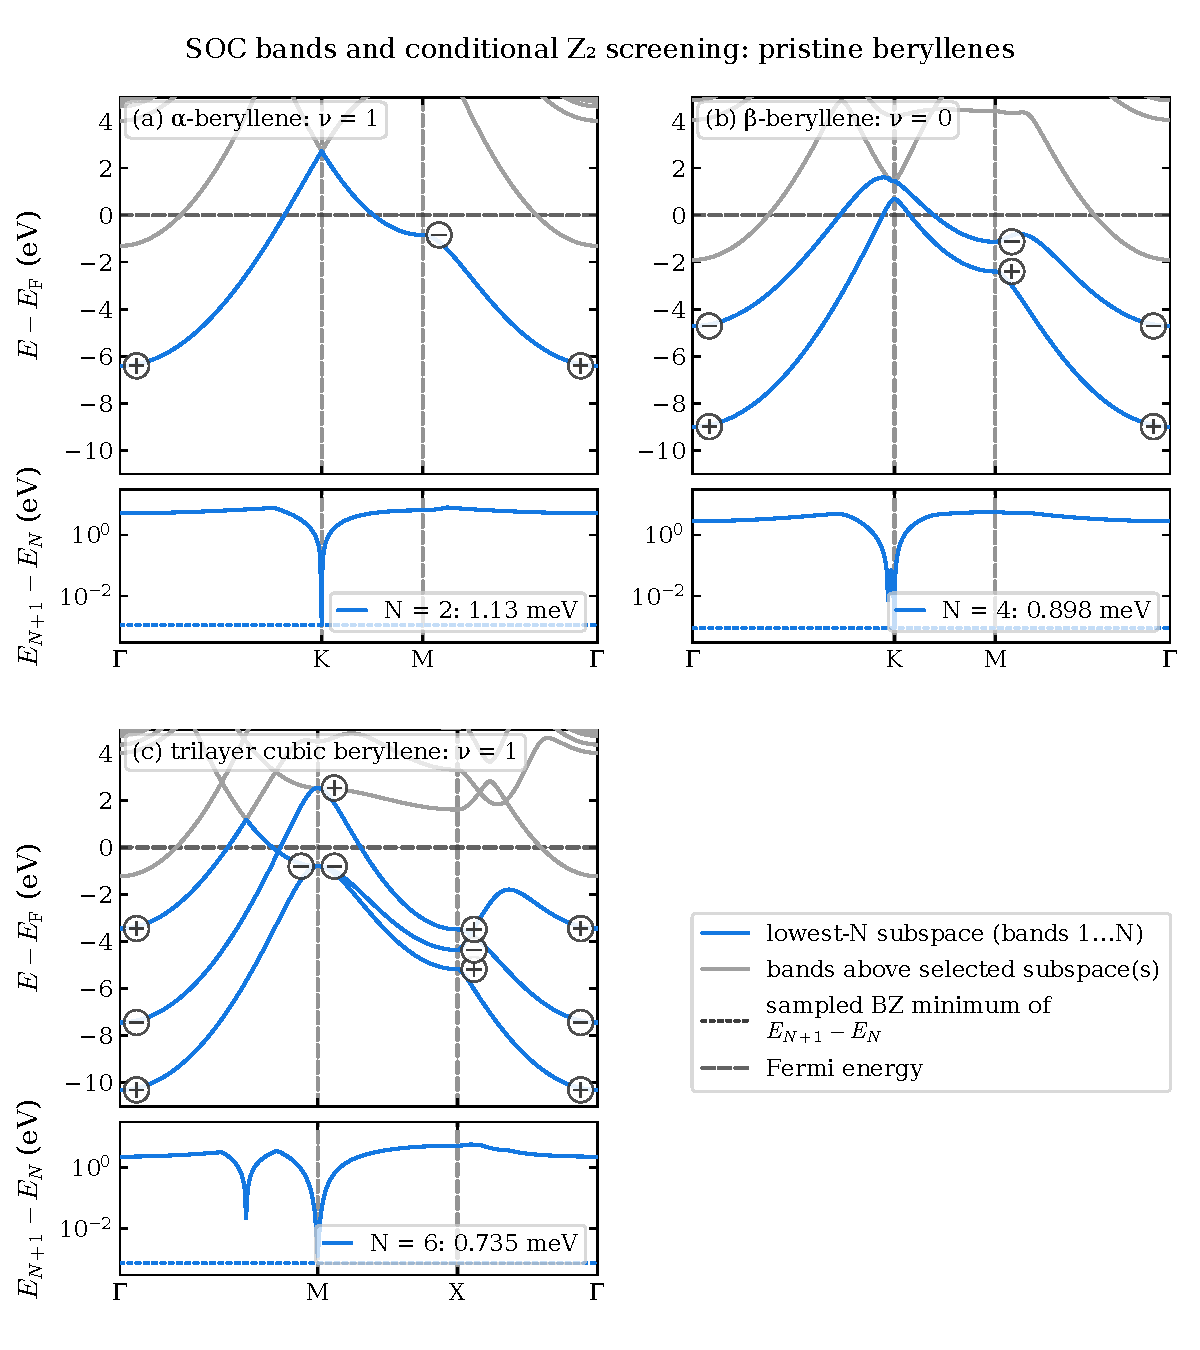
\includegraphics[width=0.80\linewidth]{figures_proj3/topology_bands_pristine_thesis.pdf}
\caption{Spin-orbit-coupled band structures of $\alpha$-beryllene, $\beta$-beryllene, and trilayer cubic beryllene.
Blue lines mark the lowest $N$ bands.
Each circled sign gives the parity of one Kramers pair at a time-reversal invariant momentum on the path.
For pairs within \qty{0.45}{\electronvolt} of each other, the signs are offset horizontally.
The lower plots show the direct gap $E_{N+1}-E_N$ along each path on a logarithmic scale and indicate the smallest gap sampled across the Brillouin zone.}
\label{fig:proj3_topology_bands_pristine}
\end{figure}

\begin{figure}[!htbp]
\centering
    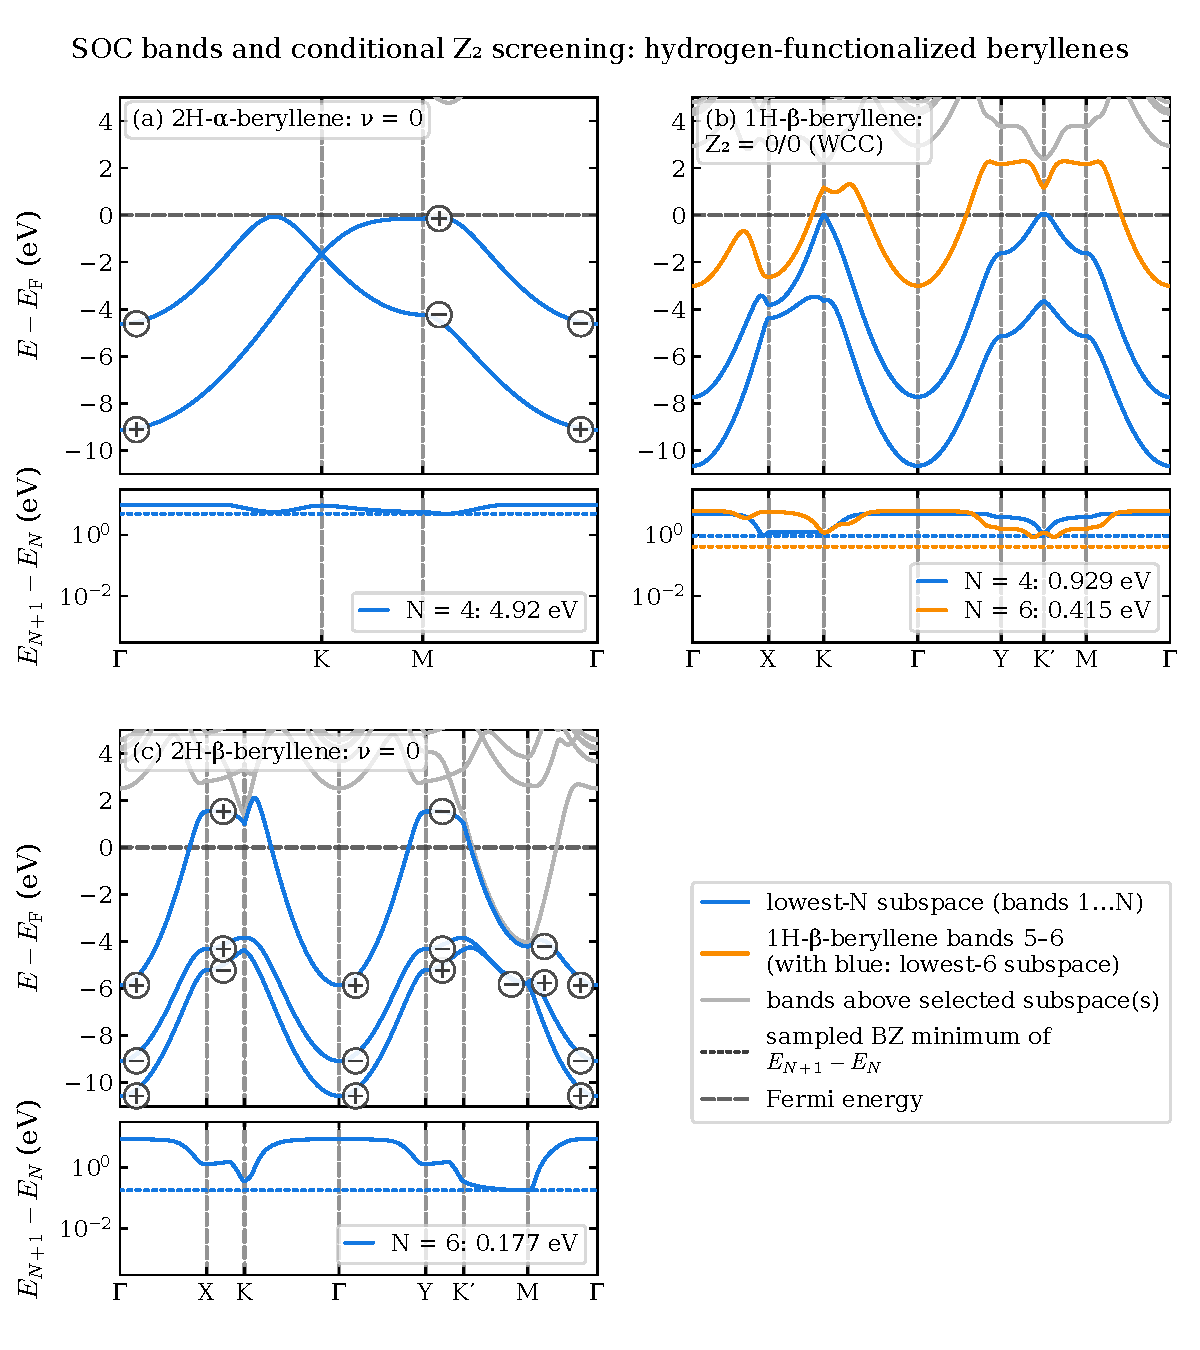
\includegraphics[width=0.80\linewidth]{figures_proj3/topology_bands_hydrogenated_thesis.pdf}
\caption{Spin-orbit-coupled band structures of 2H-$\alpha$-beryllene, 1H-$\beta$-beryllene, and 2H-$\beta$-beryllene, shown as in figure~\ref{fig:proj3_topology_bands_pristine}.
For 1H-$\beta$-beryllene, blue lines mark bands 1--4 and orange lines mark bands 5 and 6.
Together, these bands define the two subspaces with $N=4$ and $N=6$.
Both $\beta$-beryllene derivatives follow the paths of figure~\ref{fig:proj3_band_structures_cubic_hydrogenated}.}
\label{fig:proj3_topology_bands_hydrogenated}
\end{figure}

\subsection{Electron-phonon coupling and superconductivity}
\label{3_superconductivity}

We now examine phonon-mediated pairing between electrons near the Fermi level in three metallic structures.
Table~\ref{tab:proj3_superconductivity} gives the coupling strength $\lambda$ and the transition temperatures estimated from the Allen--Dynes expression and the Migdal--Eliashberg equations.
Figure~\ref{fig:proj3_superconducting_gap} shows the calculated gaps.

For trilayer cubic beryllene, phonons above \qty{40}{\per\centi\metre} give $\lambda=0.46$.
For $\mu^*=0.13$, we obtain $T_\mathrm{c}^{\mathrm{AD}}=\qty{2.0}{\kelvin}$ and $T_\mathrm{c}^{\mathrm{iso}}=\qty{3.7}{\kelvin}$.
The fitted gap ratio of 3.58 is close to the weak-coupling Bardeen--Cooper--Schrieffer value of 3.53~\cite{bardeen1957theory}.

With the same threshold, 2H-$\beta$-beryllene has the strongest coupling, $\lambda=1.40$.
At $\mu^*=0.13$, the Allen--Dynes expression gives $T_\mathrm{c}^{\mathrm{AD}}=\qty{21.9}{\kelvin}$.
The isotropic solution in figure~\ref{fig:proj3_superconducting_gap}(c) gives $T_\mathrm{c}^{\mathrm{iso}}=\qty{28.3}{\kelvin}$.
Its fitted gap ratio of 4.28 exceeds the weak-coupling value.
Figure~\ref{fig:proj3_superconducting_gap}(d) shows that the anisotropic gap approaches a finite value during the iterations at \qtyrange{29}{31}{\kelvin}.
At the sampled temperatures from \qty{32}{\kelvin} to \qty{38}{\kelvin}, the gap decays towards zero.
Extrapolating the gap and its decay rate gives $T_\mathrm{c}^{\mathrm{aniso}}\approx\qty{31.7}{\kelvin}$, between \qty{31}{\kelvin} and \qty{32}{\kelvin}.

For 2H-$\beta$-beryllene, these results use the structure relaxed with the D3 dispersion correction and exclude phonon frequencies below \qty{40}{\per\centi\metre}.
The lattice constant is \qty{2.4}{\percent} smaller than the PBE value in table~\ref{tab:proj3_hydrogenated_structural_parameters}.
On the coarse $12 \times 12 \times 1$ mesh, the only imaginary frequency is $0.24\mathrm{i}$~\si{\tera\hertz} at $\Gamma$.
The soft-mode wave vector of the PBE structure in section~\ref{3_dynamical_stability_and_phonon_dispersion} lies between the sampled wave vectors of this mesh.
At the nearest sampled wave vector, the lowest frequency is \qty{5.9}{\tera\hertz}.

For 1H-$\beta$-beryllene at $\mu^*=0.13$, the Allen--Dynes expression gives $T_\mathrm{c}^{\mathrm{AD}}=\qty{8.1}{\kelvin}$.
The isotropic solution gives $T_\mathrm{c}^{\mathrm{iso}}=\qty{11.6}{\kelvin}$ and a fitted gap ratio of 3.64.
In figure~\ref{fig:proj3_superconducting_gap}(b), the anisotropic gap approaches a finite value at \qty{14.0}{\kelvin} and \qty{14.1}{\kelvin}.
At the sampled temperatures from \qty{14.5}{\kelvin} to \qty{17.0}{\kelvin}, the gap decays towards zero.
We obtain limiting gaps of \qtyrange{0.39}{0.40}{\milli\electronvolt} at \qty{14.0}{\kelvin} and \qtyrange{0.25}{0.28}{\milli\electronvolt} at \qty{14.1}{\kelvin}.
At \qty{14.2}{\kelvin}, the gap is still decreasing after about 5000 iterations.
We therefore estimate $T_\mathrm{c}^{\mathrm{aniso}}$ at \qty{14.2}{\kelvin}, within the bracket of \qtyrange{14.1}{14.5}{\kelvin}.

Consequently, we arrive at the conclusion that the gap anisotropy raises the transition temperatures of both hydrogen-functionalized metallic layers.
These temperatures mark the closing of the calculated superconducting gap.
A separate calculation of the superfluid stiffness determines the transition associated with the loss of phase coherence in two dimensions.

\begin{table}[!htbp]
\centering
\rowcolors{2}{gray!15}{white}
\begin{adjustbox}{max width=1.0\linewidth,center}
\begin{tabular}{cccccccc}
\hline
\rowcolor{gray!25}
structure
& $\lambda$
& $\hbar\omega_\mathrm{log}$ (meV)
& $T_\mathrm{c}^{\mathrm{AD}}$ (K)
& $T_\mathrm{c}^{\mathrm{iso}}$ (K)
& $\Delta_0$ (meV)
& $2\Delta_0/(\kB T_\mathrm{c}^{\mathrm{iso}})$
& $T_\mathrm{c}^{\mathrm{aniso}}$ (K) \\
\hline
trilayer cubic beryllene
& 0.46 & 36.0 & 3.7 / 2.0 / 0.9 & 3.7 & 0.57 & 3.58 & -- \\
2H-$\beta$-beryllene
& 1.40 & 19.5 & 24.2 / 21.9 / 19.6 & 28.3 & 5.23 & 4.28 & $\approx 31.7$ \\
1H-$\beta$-beryllene
& 0.61 & 40.7 & 11.4 / 8.1 / 5.4 & 11.6 & 1.83 & 3.64 & $\approx 14.2$ \\
\hline
\end{tabular}
\end{adjustbox}
\caption{Electron-phonon coupling strength $\lambda$, logarithmic average phonon energy $\hbar\omega_\mathrm{log}$, and estimated superconducting transition temperatures.
The Allen--Dynes values $T_\mathrm{c}^{\mathrm{AD}}$ follow from equation~\eqref{allen_dynes_temperature_estimate} for $\mu^*=0.10$, 0.13, and 0.16, respectively.
The gap amplitude $\Delta_0$ and the gap ratio refer to the isotropic Migdal--Eliashberg fit.
The isotropic and anisotropic solutions use $\mu^*=0.13$.
All calculations use $80 \times 80 \times 1$ fine meshes and the phonon frequency thresholds given in section~\ref{3_methods}.
The dash indicates that we did not calculate an anisotropic solution for the trilayer.}
\label{tab:proj3_superconductivity}
\end{table}

\begin{figure}[!htbp]
\centering
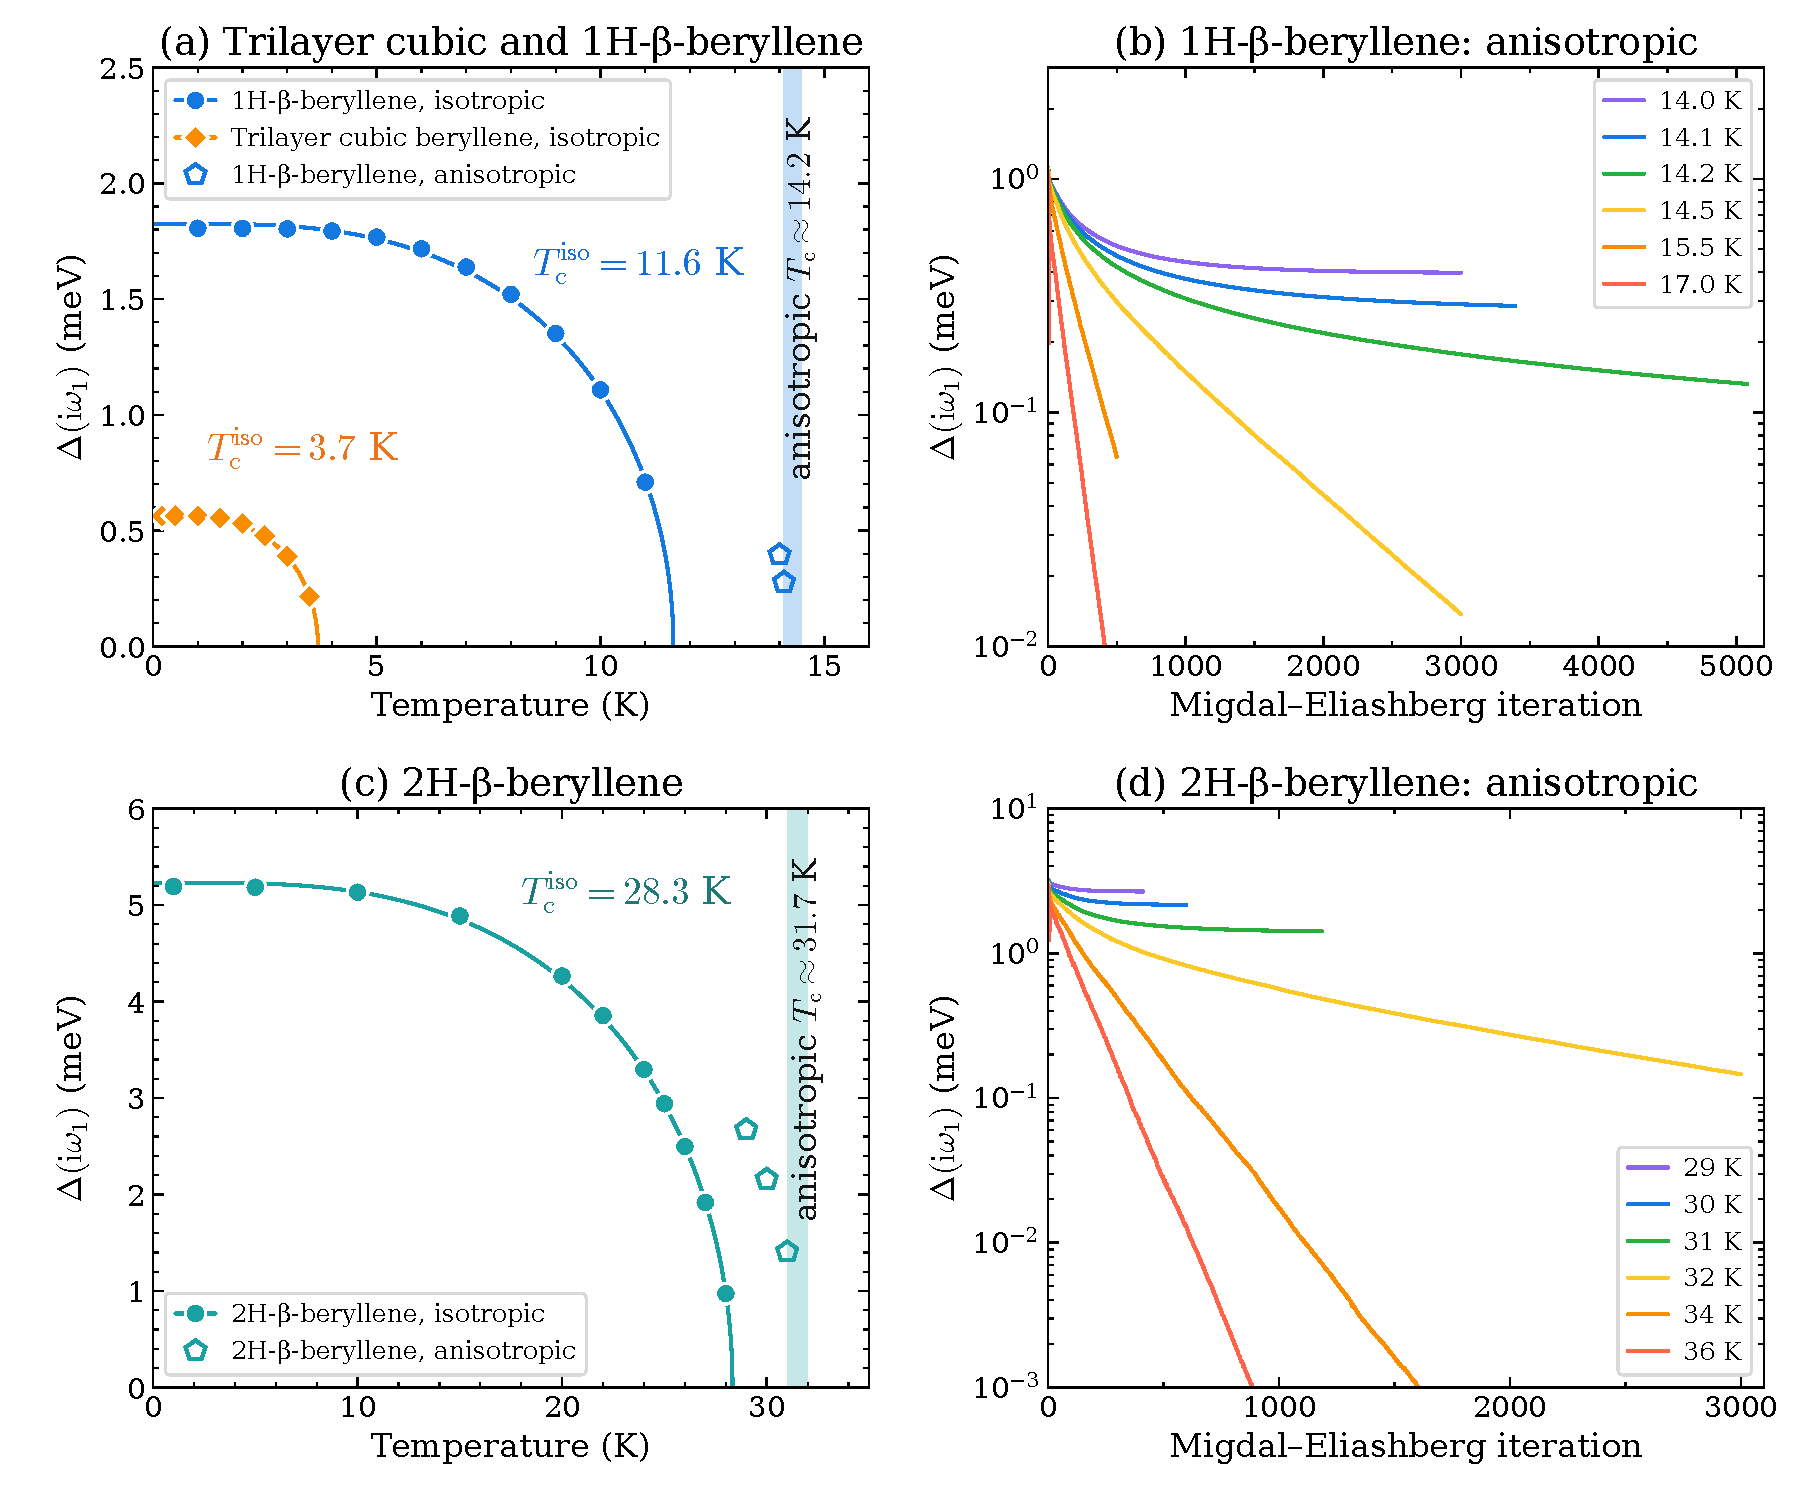
\includegraphics[width=0.80\linewidth]{figures_proj3/superconductivity/superconductivity.pdf}
\caption{Superconducting gap $\Delta(\mathrm{i}\omega_1)$ at the first Matsubara frequency $\omega_1=\mathrm{\pi}\kB T/\hbar$.
Panels (a) and (c) show the temperature dependence.
Filled circles and diamonds mark the isotropic solutions for the hydrogenated phases and the cubic trilayer, respectively.
The curves show fits to $\Delta_0\tanh[1.74(T_\mathrm{c}^{\mathrm{iso}}/T-1)^{1/2}]$.
Panels (b) and (d) show the Fermi-surface-averaged gap during anisotropic iterations for 1H- and 2H-$\beta$-beryllene, respectively.
Each shows seven temperatures, from violet at the lowest to red at the highest.
Open pentagons in (a) and (c) mark the extrapolated limiting gaps, and shading brackets $T_\mathrm{c}^{\mathrm{aniso}}$.}
\label{fig:proj3_superconducting_gap}
\end{figure}

\subsection{Optical properties}
\label{3_optical_properties}

We now compare the interband optical response of the beryllene structures with that of bulk hcp and bulk bcc beryllium.
As described in section~\ref{3_methods}, we derive scalar optical quantities from the Cartesian diagonal components $\varepsilon_{\lambda\lambda}(\omega)$.
We first compare pristine $\alpha$- and $\beta$-beryllene, then examine the effects of layer thickness and hydrogen adsorption.
Peak energies refer to sampled points within \qtyrange{0}{12}{\electronvolt}.
We locate zero crossings and refractive-index crossings by linear interpolation between adjacent samples.

\subsubsection{Pristine $\alpha$- and $\beta$-beryllene}
\label{3_optical_alpha_beta}

Figure~\ref{fig:proj3_alpha_beta_dielectric} shows the real and imaginary parts of the dielectric function for pristine $\alpha$- and $\beta$-beryllene.
For $\beta$-beryllene, the sampled in-plane and out-of-plane real parts have opposite signs over \qtyrange{1.22}{2.21}{\electronvolt}.
For $\alpha$-beryllene, the out-of-plane real part crosses zero near \qty{10.64}{\electronvolt}, where the imaginary part is small.
These features identify energy ranges for testing collective modes.
A finite-momentum response calculation determines their propagation and lifetimes.

\begin{figure}[!htbp]
\centering
    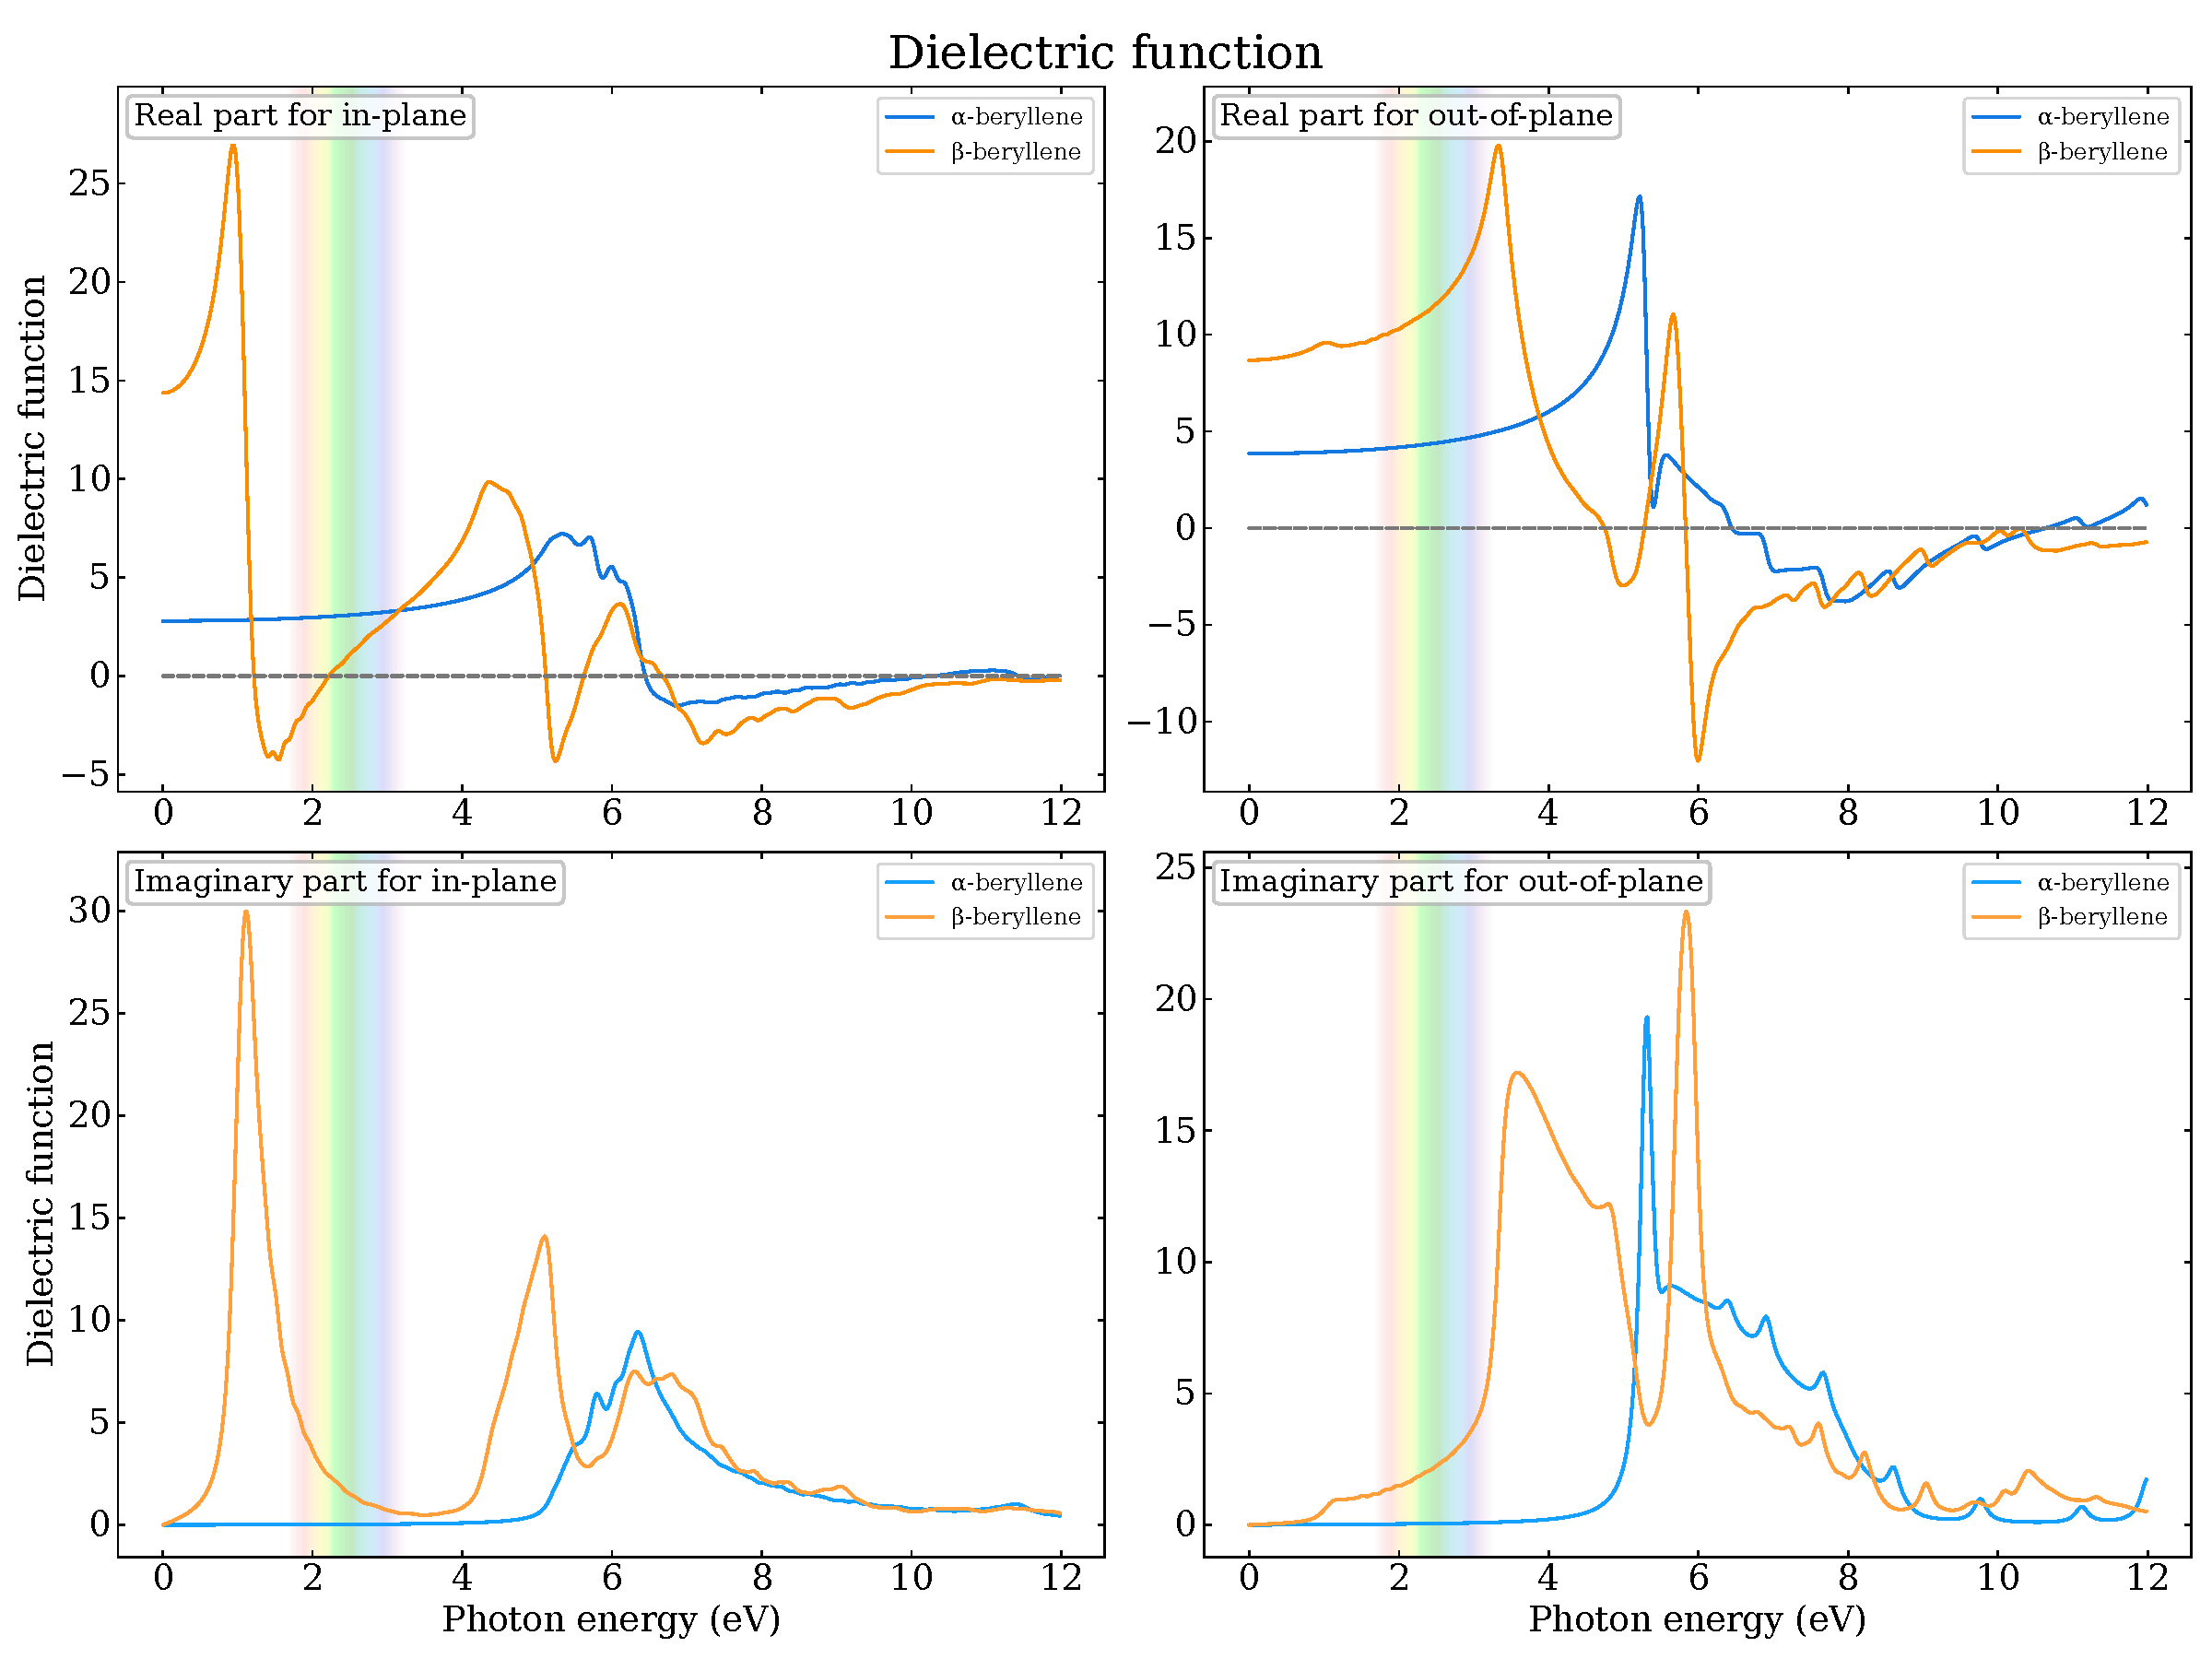
\includegraphics[width=0.80\linewidth]{figures_proj3/dielectric_alpha-beta_thesis.pdf}
\caption{Real and imaginary parts of the dielectric function for $\alpha$-beryllene and $\beta$-beryllene.
The spectra are shown for the in-plane and out-of-plane directions as functions of photon energy.
The in-plane and out-of-plane curves correspond to the $xx$ and $zz$ components, respectively.}
\label{fig:proj3_alpha_beta_dielectric}
\end{figure}

The absorption coefficient $\alpha_{\lambda}(\omega)$ has a larger sampled maximum in $zz$ than in $xx$ for both phases, as shown in figure~\ref{fig:proj3_alpha_beta_abs_refractive}.
For $\alpha$-beryllene, the maxima are \qty{0.135}{\per\nano\metre} in $xx$ and \qty{0.175}{\per\nano\metre} in $zz$.
For $\beta$-beryllene, they are \qty{0.161}{\per\nano\metre} and \qty{0.242}{\per\nano\metre}, respectively, with the $zz$ maximum near \qty{5.95}{\electronvolt}.
The ordering of the two phases varies with photon energy because their spectra cross.

The in-plane refractive index $n_x(\omega)$ of $\beta$-beryllene peaks in the infrared and ultraviolet, with a minimum between them.
The corresponding $\alpha$-beryllene spectrum varies more smoothly across this region.
The $xx$ and $zz$ components of $\alpha$-beryllene first cross $n=1$ downwards near \qty{7.41}{\electronvolt} and \qty{7.82}{\electronvolt}, respectively.
For $\beta$-beryllene, the corresponding crossings occur at \qty{7.33}{\electronvolt} and \qty{6.37}{\electronvolt}.
The out-of-plane index of $\alpha$-beryllene rises above one again near \qty{11.71}{\electronvolt}.

\begin{figure}[!htbp]
\centering
    \adjustbox{valign=c}{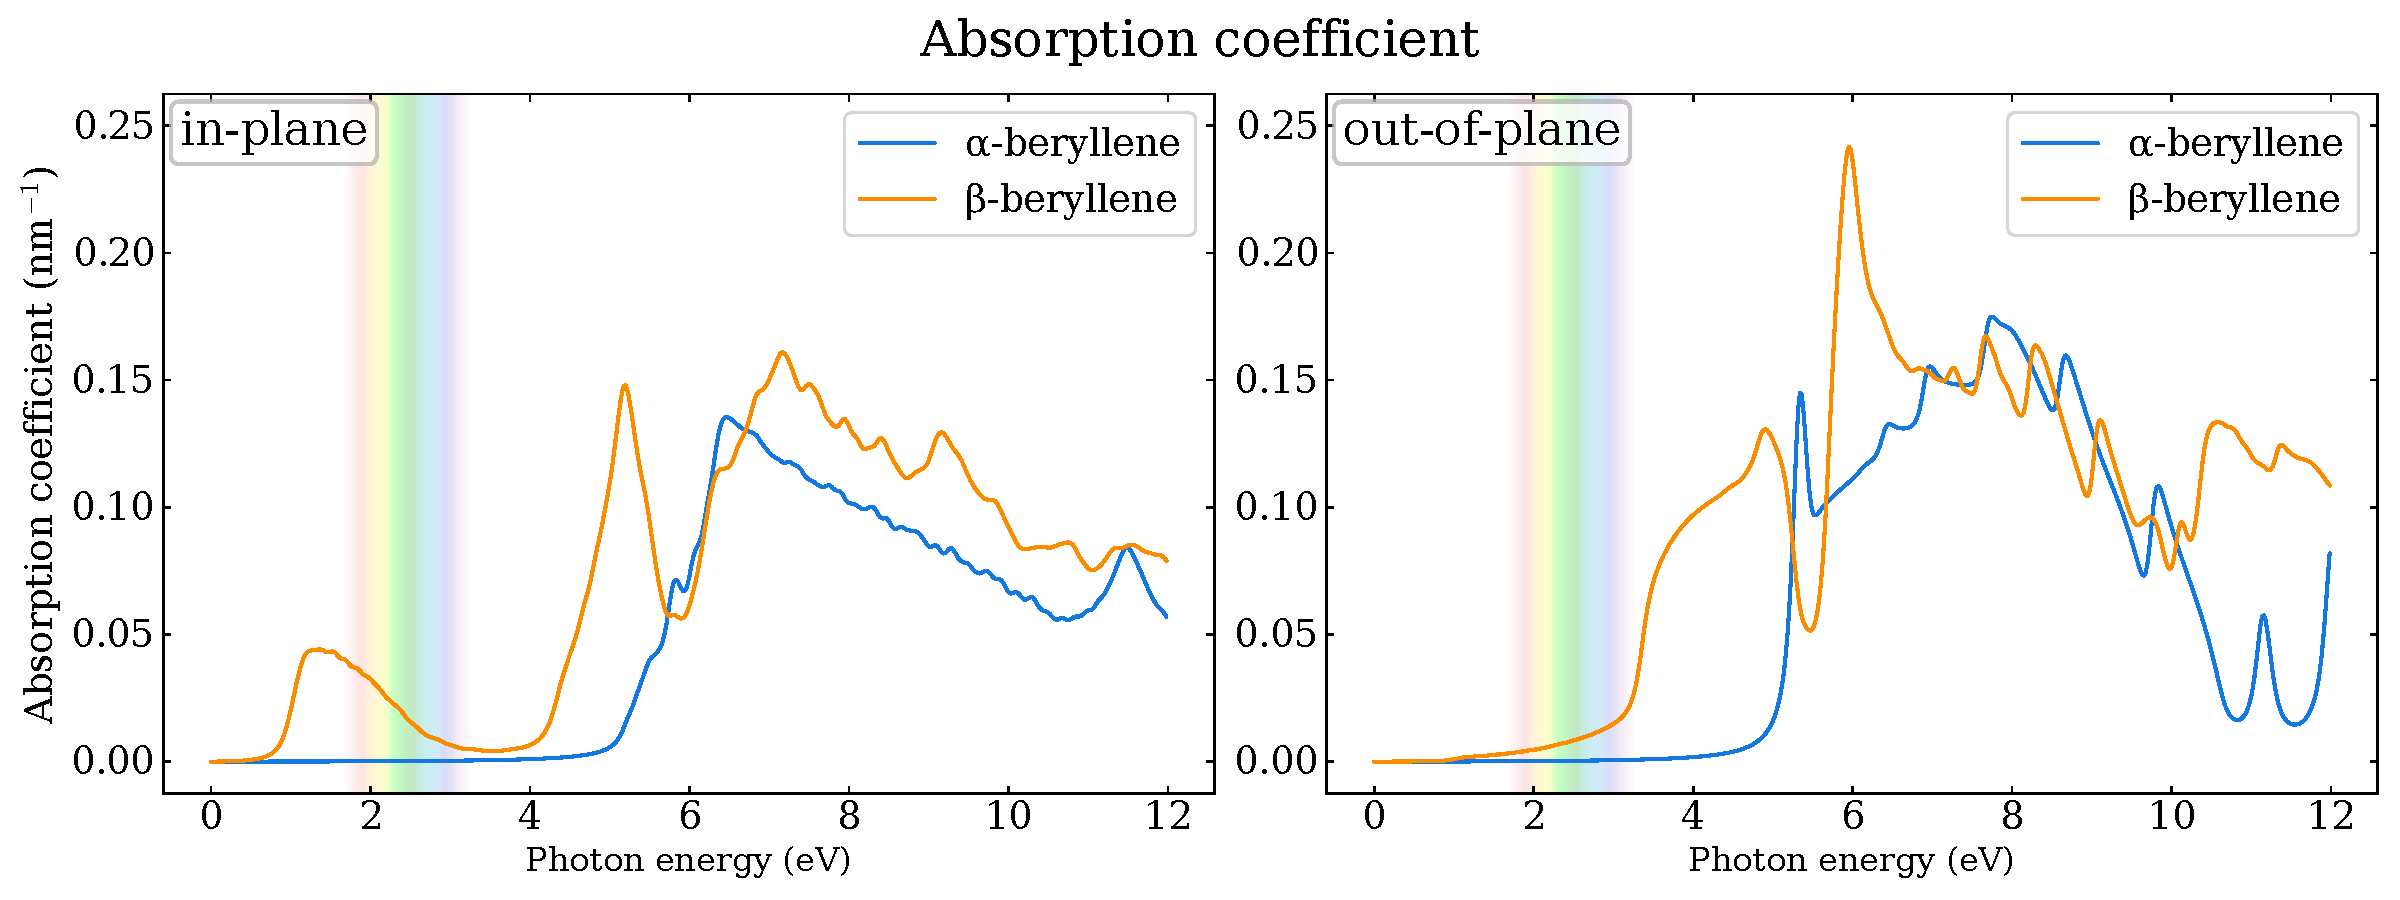
\includegraphics[width=0.80\linewidth]{figures_proj3/optics_alpha-beta_absorption_thesis.pdf}}%
    \par\nointerlineskip
    \adjustbox{valign=c}{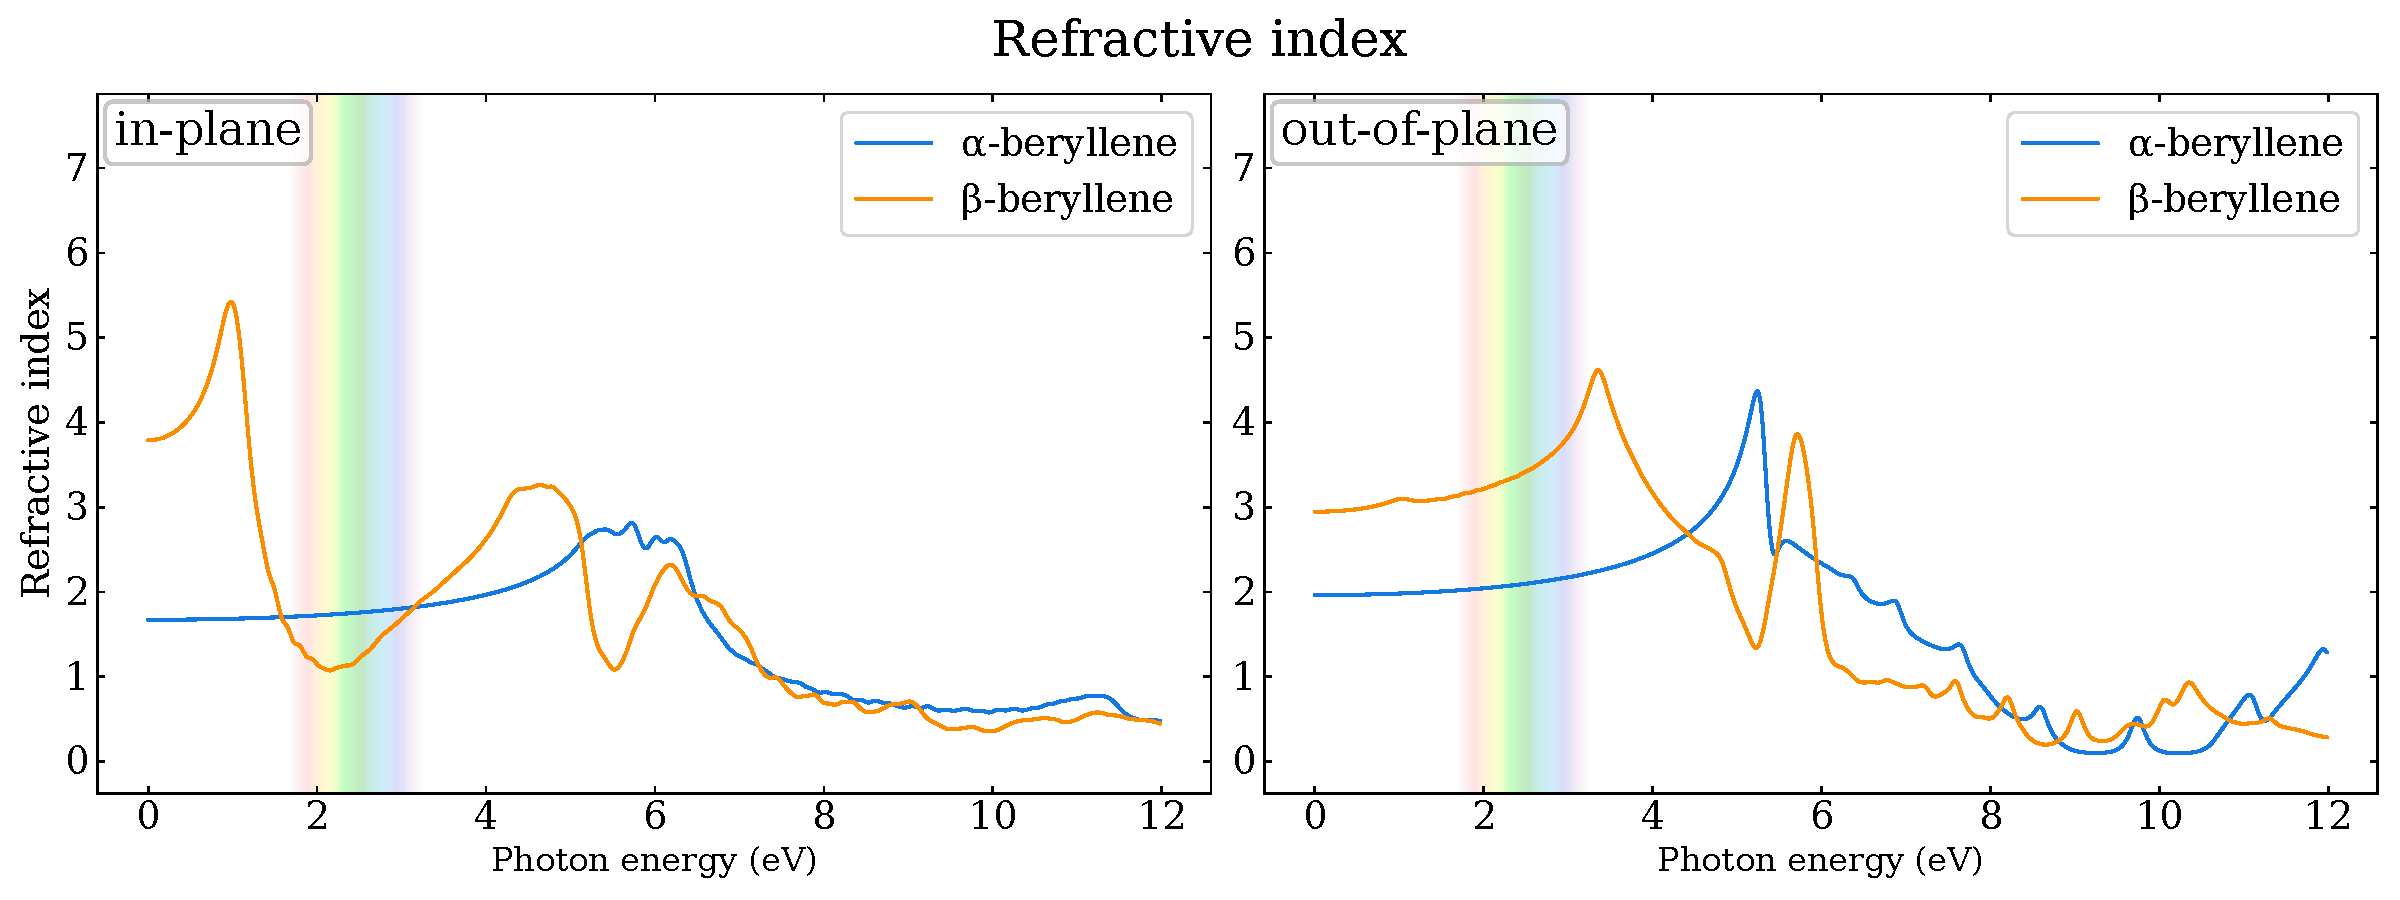
\includegraphics[width=0.80\linewidth]{figures_proj3/optics_alpha-beta_refractive_thesis.pdf}}%
\caption{Absorption coefficient and refractive index of $\alpha$-beryllene and $\beta$-beryllene.
Upper: absorption coefficient (\unit{\per\nano\metre}). Lower: refractive index.
The spectra are shown for the in-plane and out-of-plane directions as functions of photon energy.
The in-plane and out-of-plane curves correspond to the $xx$ and $zz$ components, respectively.}
\label{fig:proj3_alpha_beta_abs_refractive}
\end{figure}

The extinction coefficient $k_{\lambda}(\omega)$ in figure~\ref{fig:proj3_alpha_beta_extinction} gives the attenuation of the wave amplitude.
The $xx$ spectrum of $\beta$-beryllene has strong infrared and ultraviolet peaks separated by a trough.
Its strongest $zz$ peak occurs near \qty{5.95}{\electronvolt}, with $k_z\approx4.00$.

\begin{figure}[!htbp]
\centering
    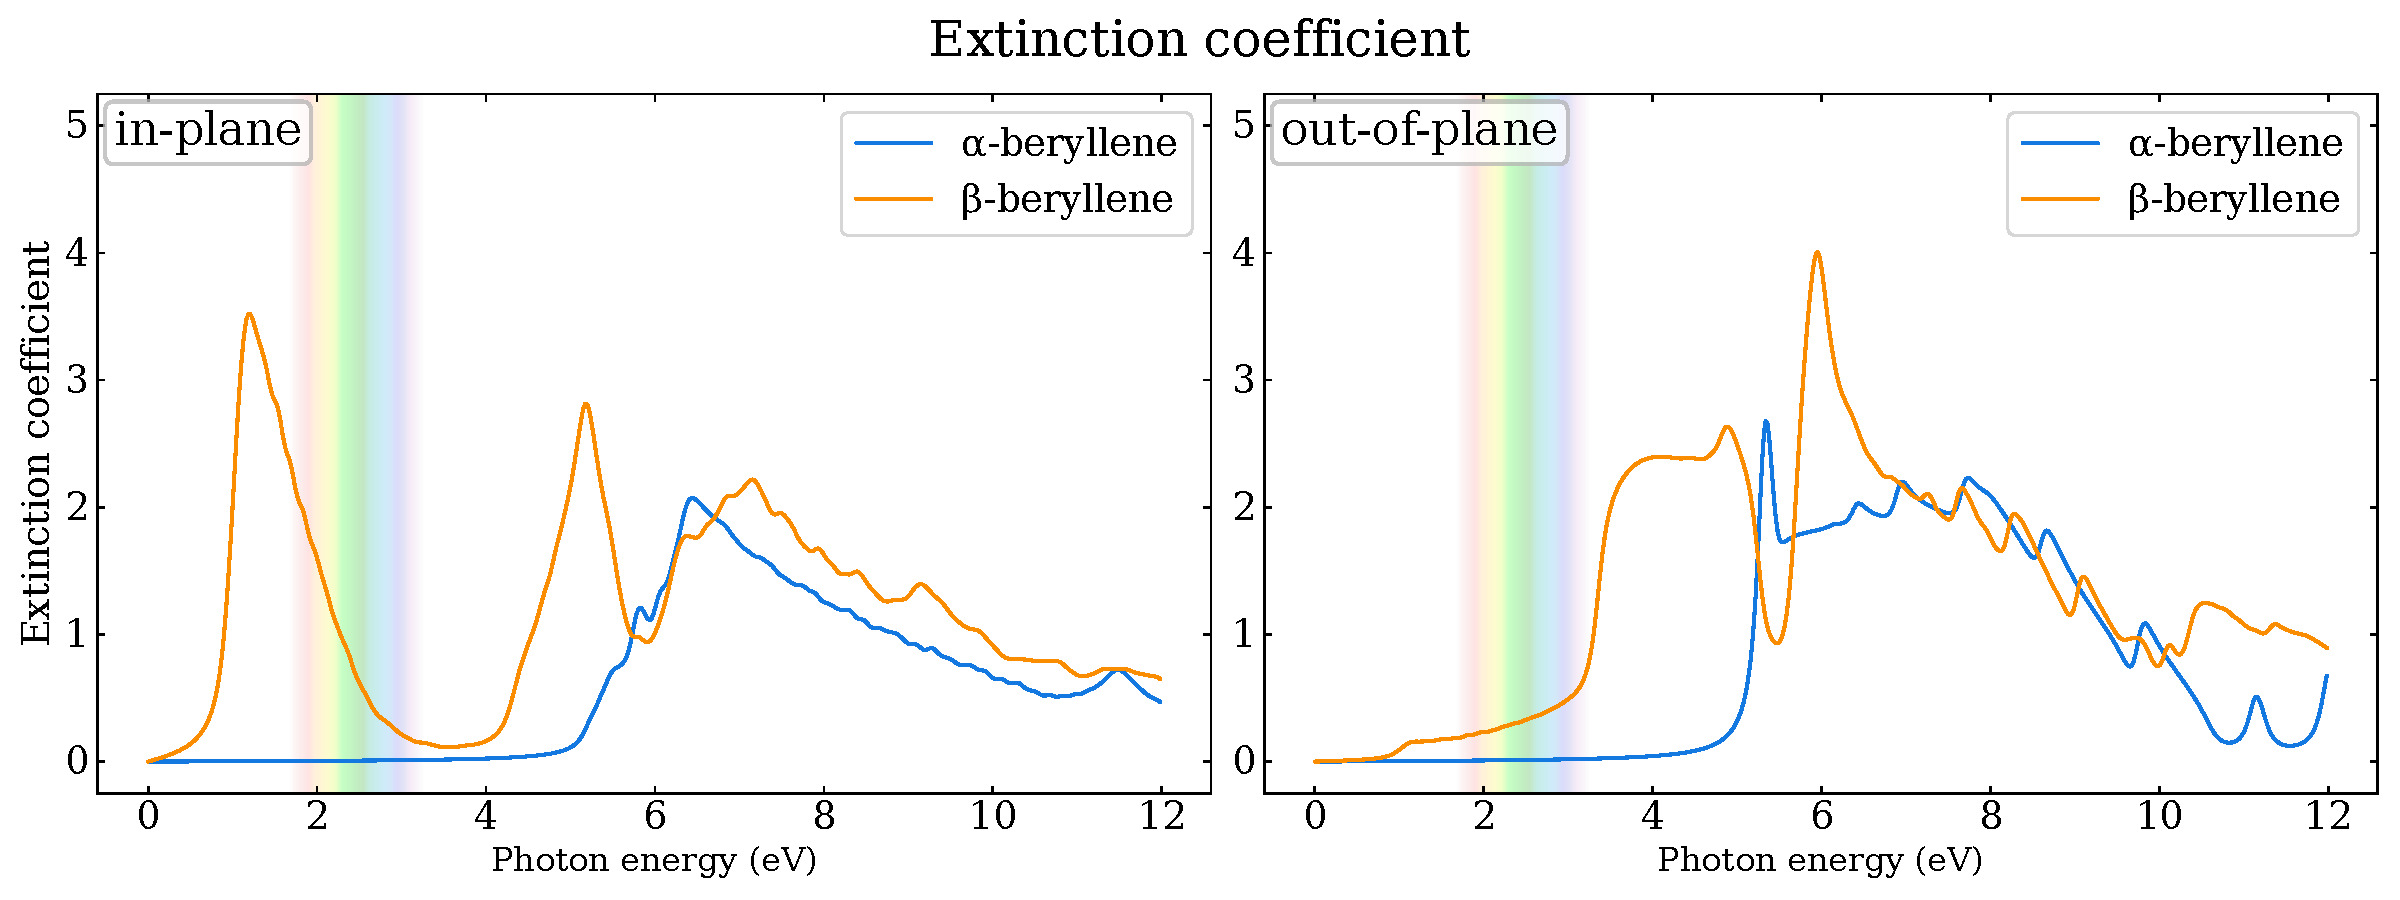
\includegraphics[width=0.80\linewidth]{figures_proj3/optics_alpha-beta_extinction_thesis.pdf}
\caption{Extinction coefficient of $\alpha$-beryllene and $\beta$-beryllene for the in-plane and out-of-plane directions as a function of photon energy.
The in-plane and out-of-plane curves correspond to the $xx$ and $zz$ components, respectively.}
\label{fig:proj3_alpha_beta_extinction}
\end{figure}

The reflectivity $R_{\lambda}(\omega)$ is shown in figure~\ref{fig:proj3_reflectivity_alpha_beta}.
The in-plane reflectivity of $\beta$-beryllene has a minimum between its infrared and ultraviolet peaks.
In the out-of-plane spectra, $\beta$-beryllene reflects more strongly at low energies, whereas $\alpha$-beryllene develops pronounced ultraviolet peaks.

Figure~\ref{fig:proj3_energy_loss_alpha_beta} compares the scalar energy-loss spectra $L_{\lambda}(\omega)$.
The $xx$ spectrum of $\beta$-beryllene has local maxima of 0.49 near \qty{2.40}{\electronvolt} and 1.34 near \qty{11.03}{\electronvolt}.
It is still rising at the final sample, where it reaches 1.50 at \qty{11.98}{\electronvolt}.
The $zz$ loss of $\alpha$-beryllene peaks at 8.88 near \qty{10.64}{\electronvolt}, close to the zero of the real dielectric component.
The corresponding $\beta$-beryllene loss peaks at 1.09 near \qty{9.95}{\electronvolt}.

\subsubsection{Bulk hcp, bulk bcc, and trilayer cubic beryllene}
\label{3_optical_bulk_cubic}

We next compare trilayer cubic beryllene with the bulk hcp and bcc references in figure~\ref{fig:proj3_bulk_cubic_dielectric}.
Cubic symmetry gives bulk bcc beryllium the same dielectric response along all three axes.
In bulk hcp beryllium, the in-plane and out-of-plane spectra differ.
Their real dielectric components become negative between \qty{4.4}{\electronvolt} and \qty{4.9}{\electronvolt}.
They reach minima between \qty{5.3}{\electronvolt} and \qty{6.2}{\electronvolt} and remain negative through the upper end of the sampled interval.
Their imaginary components show broad interband features that decay rapidly near \qty{6}{\electronvolt}.

The trilayer breaks the directional equivalence of the cubic bulk response.
Its imaginary dielectric maxima are approximately 19.75 near \qty{3.74}{\electronvolt} in $xx$ and $yy$, and 27.32 near \qty{2.71}{\electronvolt} in $zz$.
The real components also cross zero at different energies.
The absorption maxima occur at different energies because the absorption coefficient depends on photon energy and on both the real and imaginary dielectric components.

\begin{figure}[!htbp]
\centering
    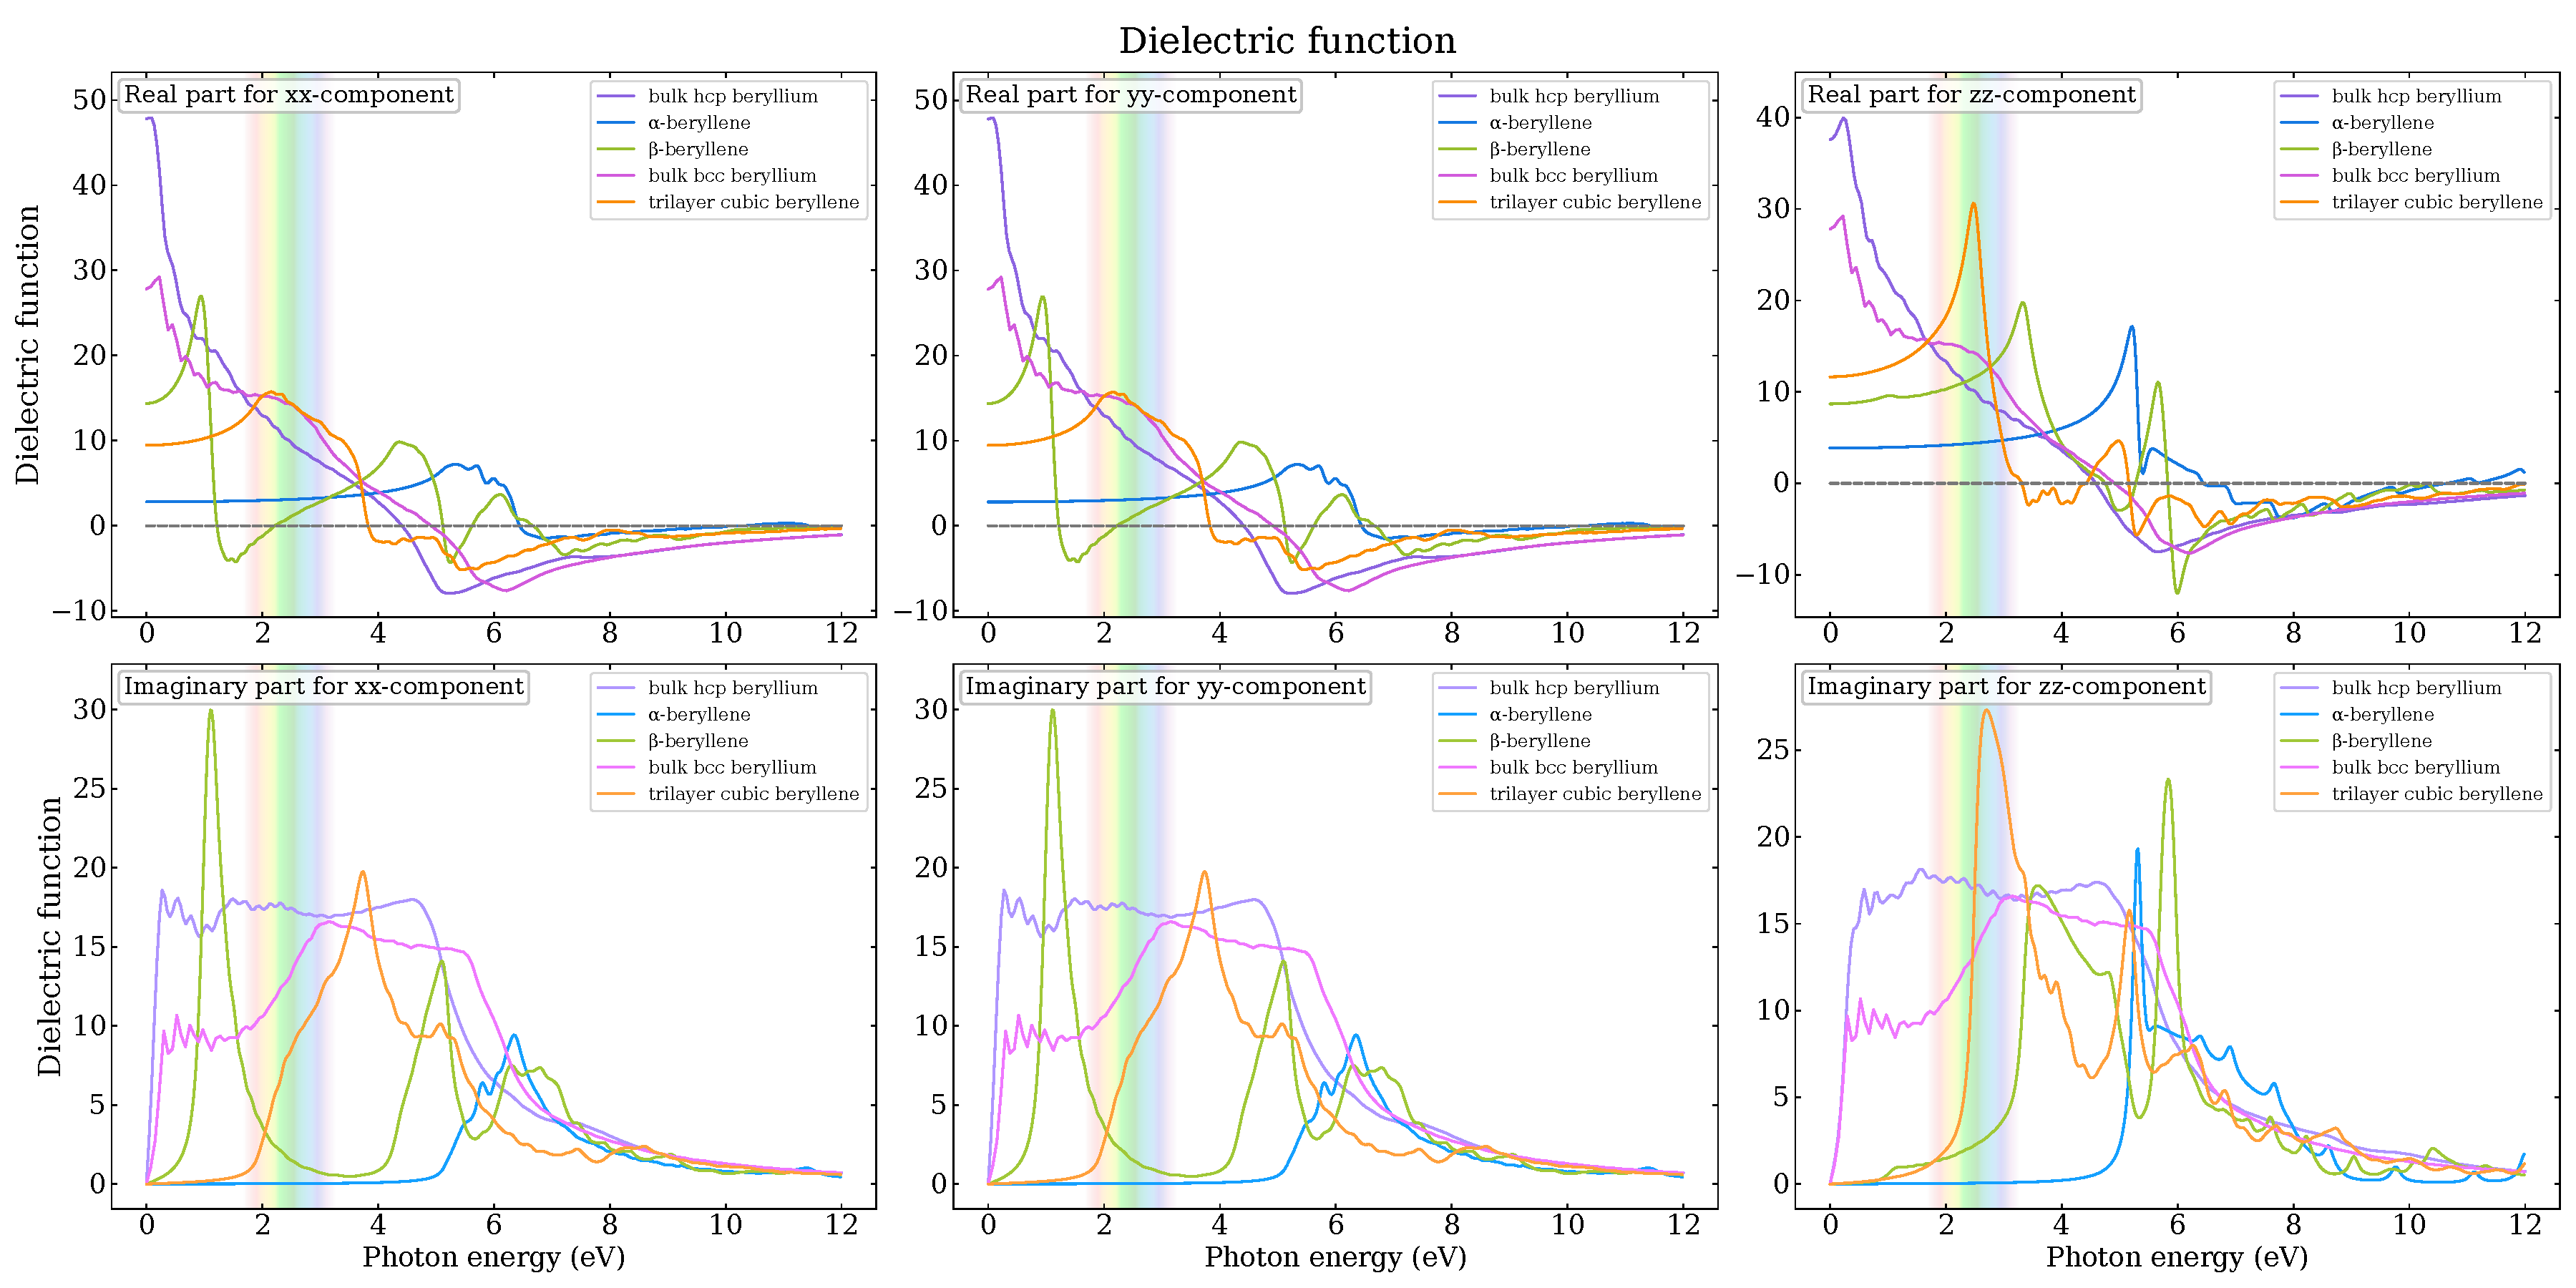
\includegraphics[width=0.95\linewidth]{figures_proj3/dielectric_pristine_thesis.pdf}
\caption{Real and imaginary parts of the dielectric function for bulk hcp beryllium,
bulk bcc beryllium,
$\alpha$-beryllene,
$\beta$-beryllene,
and trilayer cubic beryllene.
The spectra are shown for the $xx$,
$yy$,
and $zz$ components as functions of photon energy.}
\label{fig:proj3_bulk_cubic_dielectric}
\end{figure}

Figure~\ref{fig:proj3_bulk_cubic_abs_loss} compares the absorption and energy-loss spectra.
We interpolate the bulk bcc spectrum to the trilayer energy grid to compare the two in the visible interval of \qtyrange{1.65}{3.26}{\electronvolt}.
In $xx$ and $yy$, the trilayer absorbs less than bulk bcc beryllium at every sampled energy.
The corresponding visible maxima are \qty{0.0604}{\per\nano\metre} for the trilayer and \qty{0.0746}{\per\nano\metre} for the bulk.
The trilayer $zz$ coefficient exceeds the bulk value over part of this interval.
The strongest trilayer absorption occurs in the ultraviolet, near \qty{5.40}{\electronvolt} in $xx$ and $yy$ and near \qty{5.25}{\electronvolt} in $zz$.
The corresponding coefficients are \qty{0.148}{\per\nano\metre} and \qty{0.166}{\per\nano\metre}, respectively.

The trilayer also has a stronger scalar energy-loss response than bulk bcc beryllium towards the upper end of the sampled range.

\begin{figure}[!htbp]
\centering
    \adjustbox{valign=c}{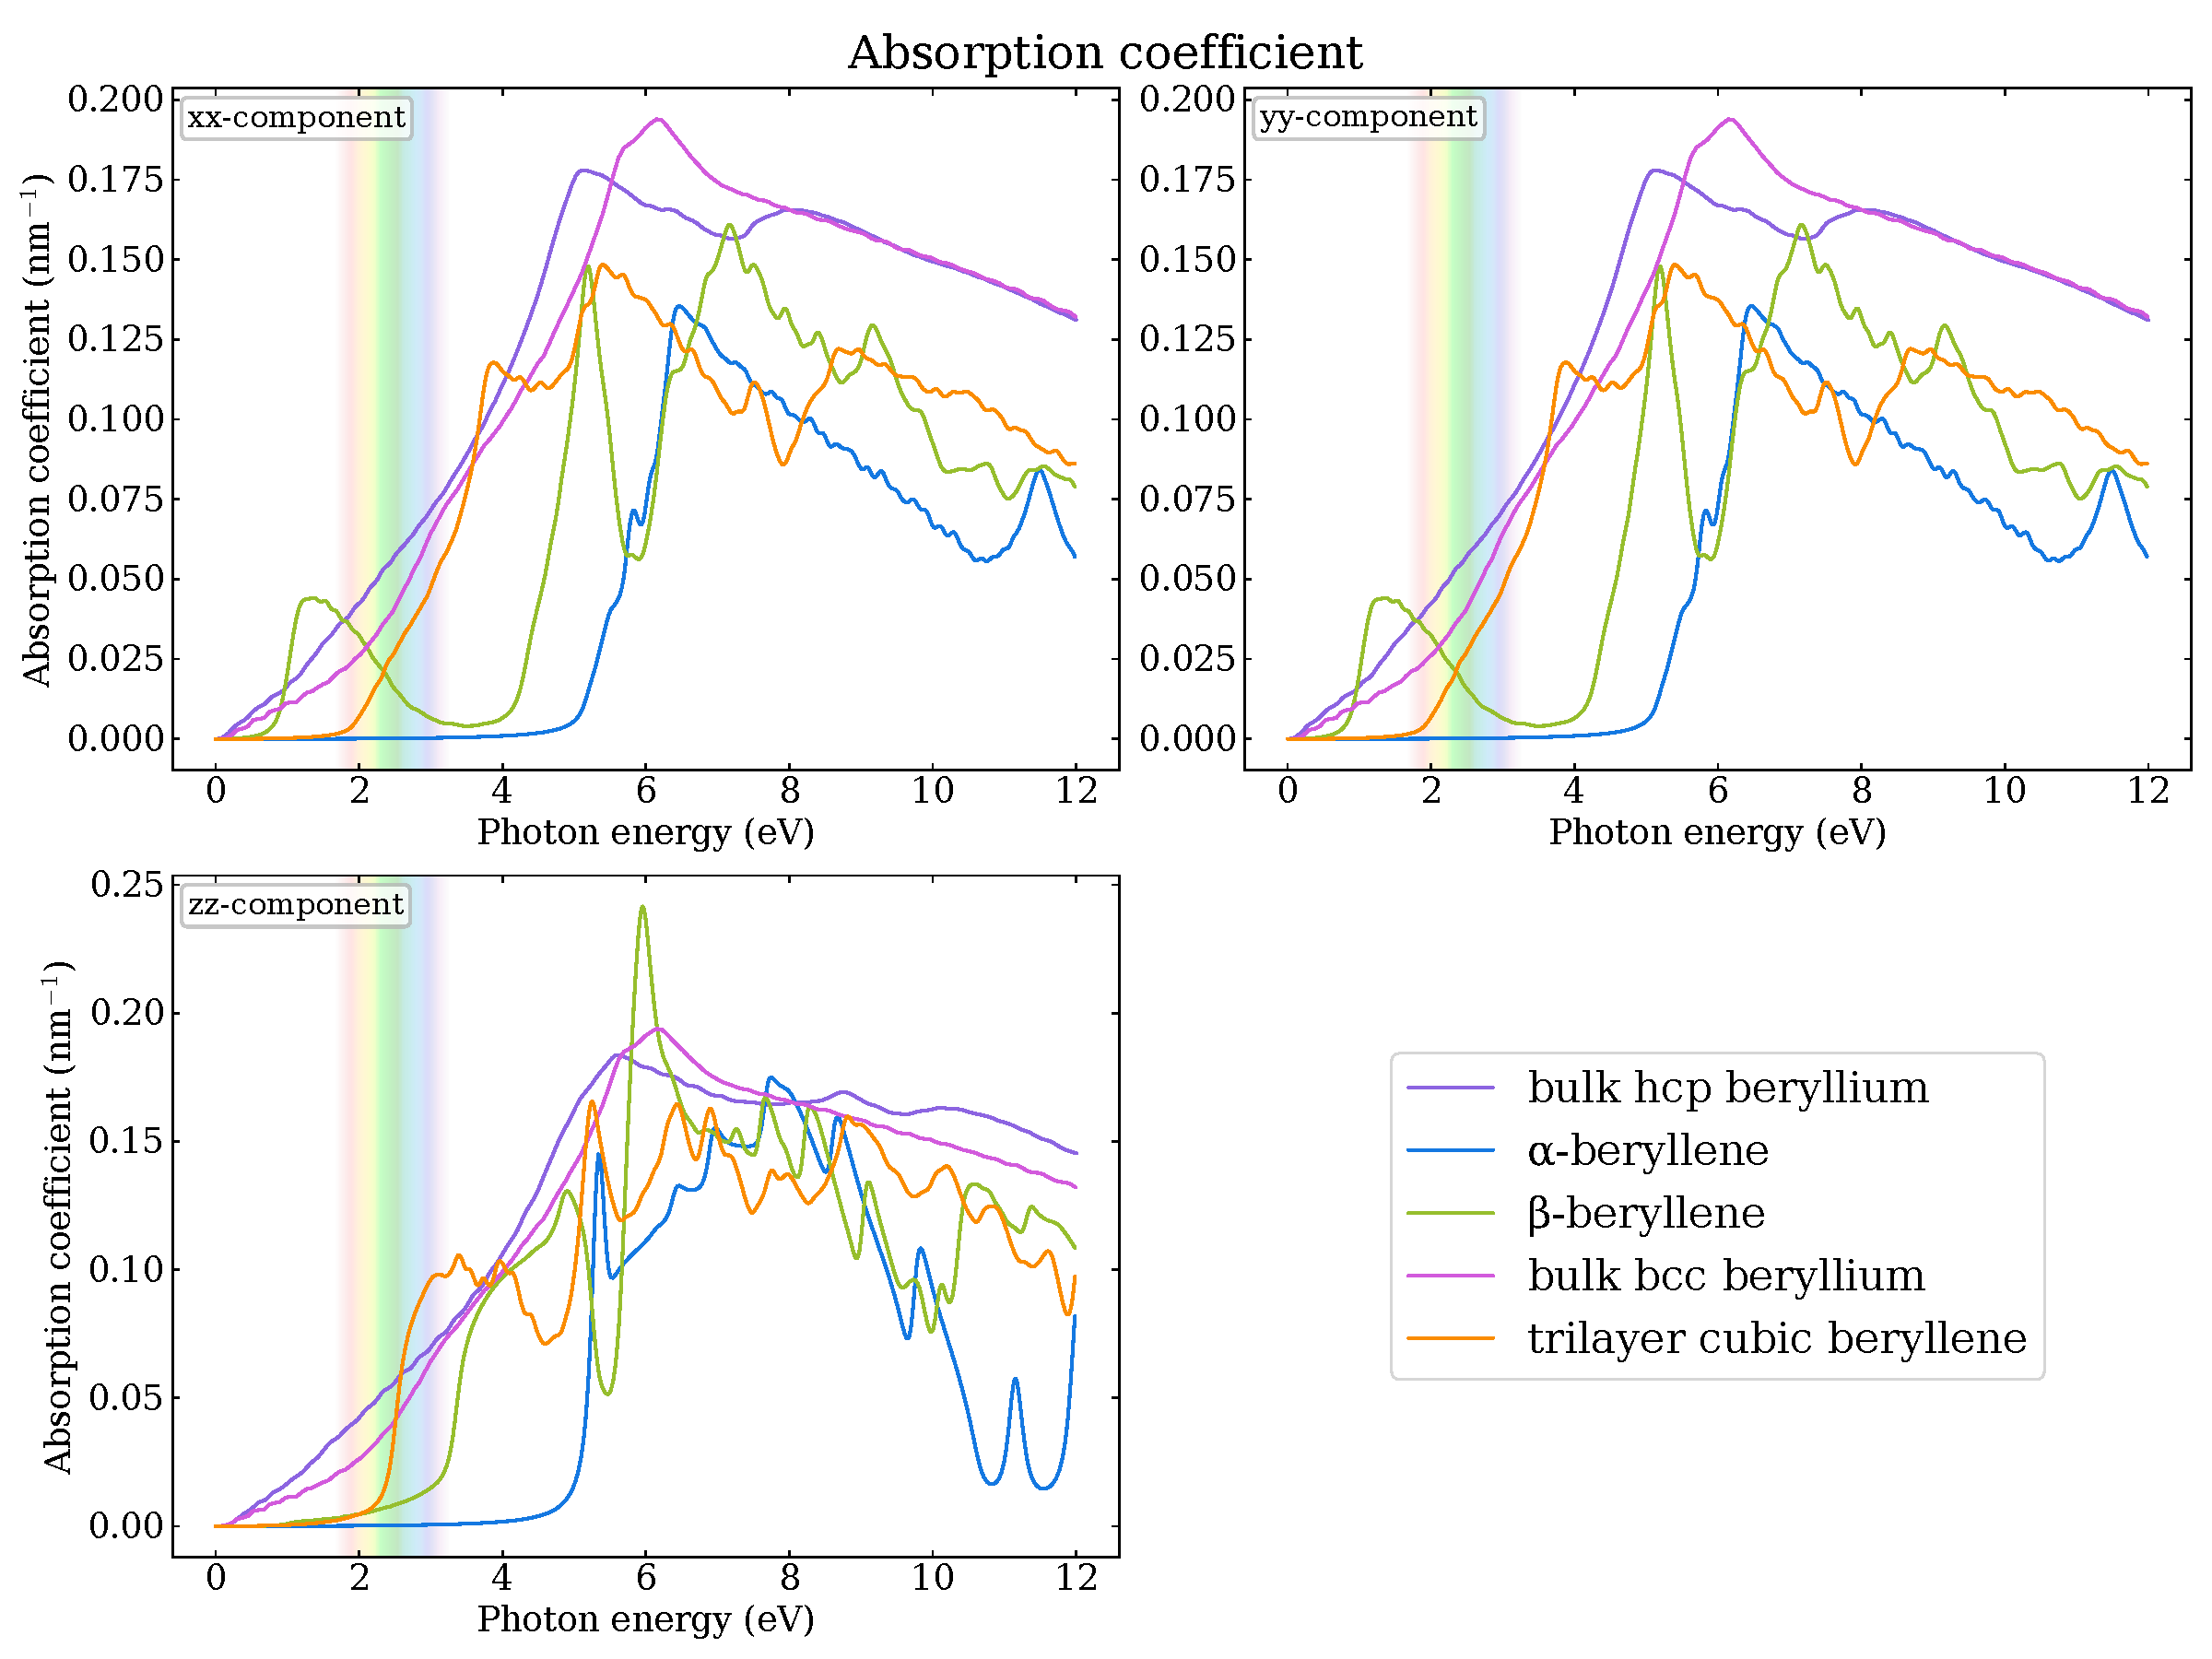
\includegraphics[width=0.80\linewidth]{figures_proj3/optics_pristine_absorption_thesis.pdf}}%
    \par\nointerlineskip
    \adjustbox{valign=c}{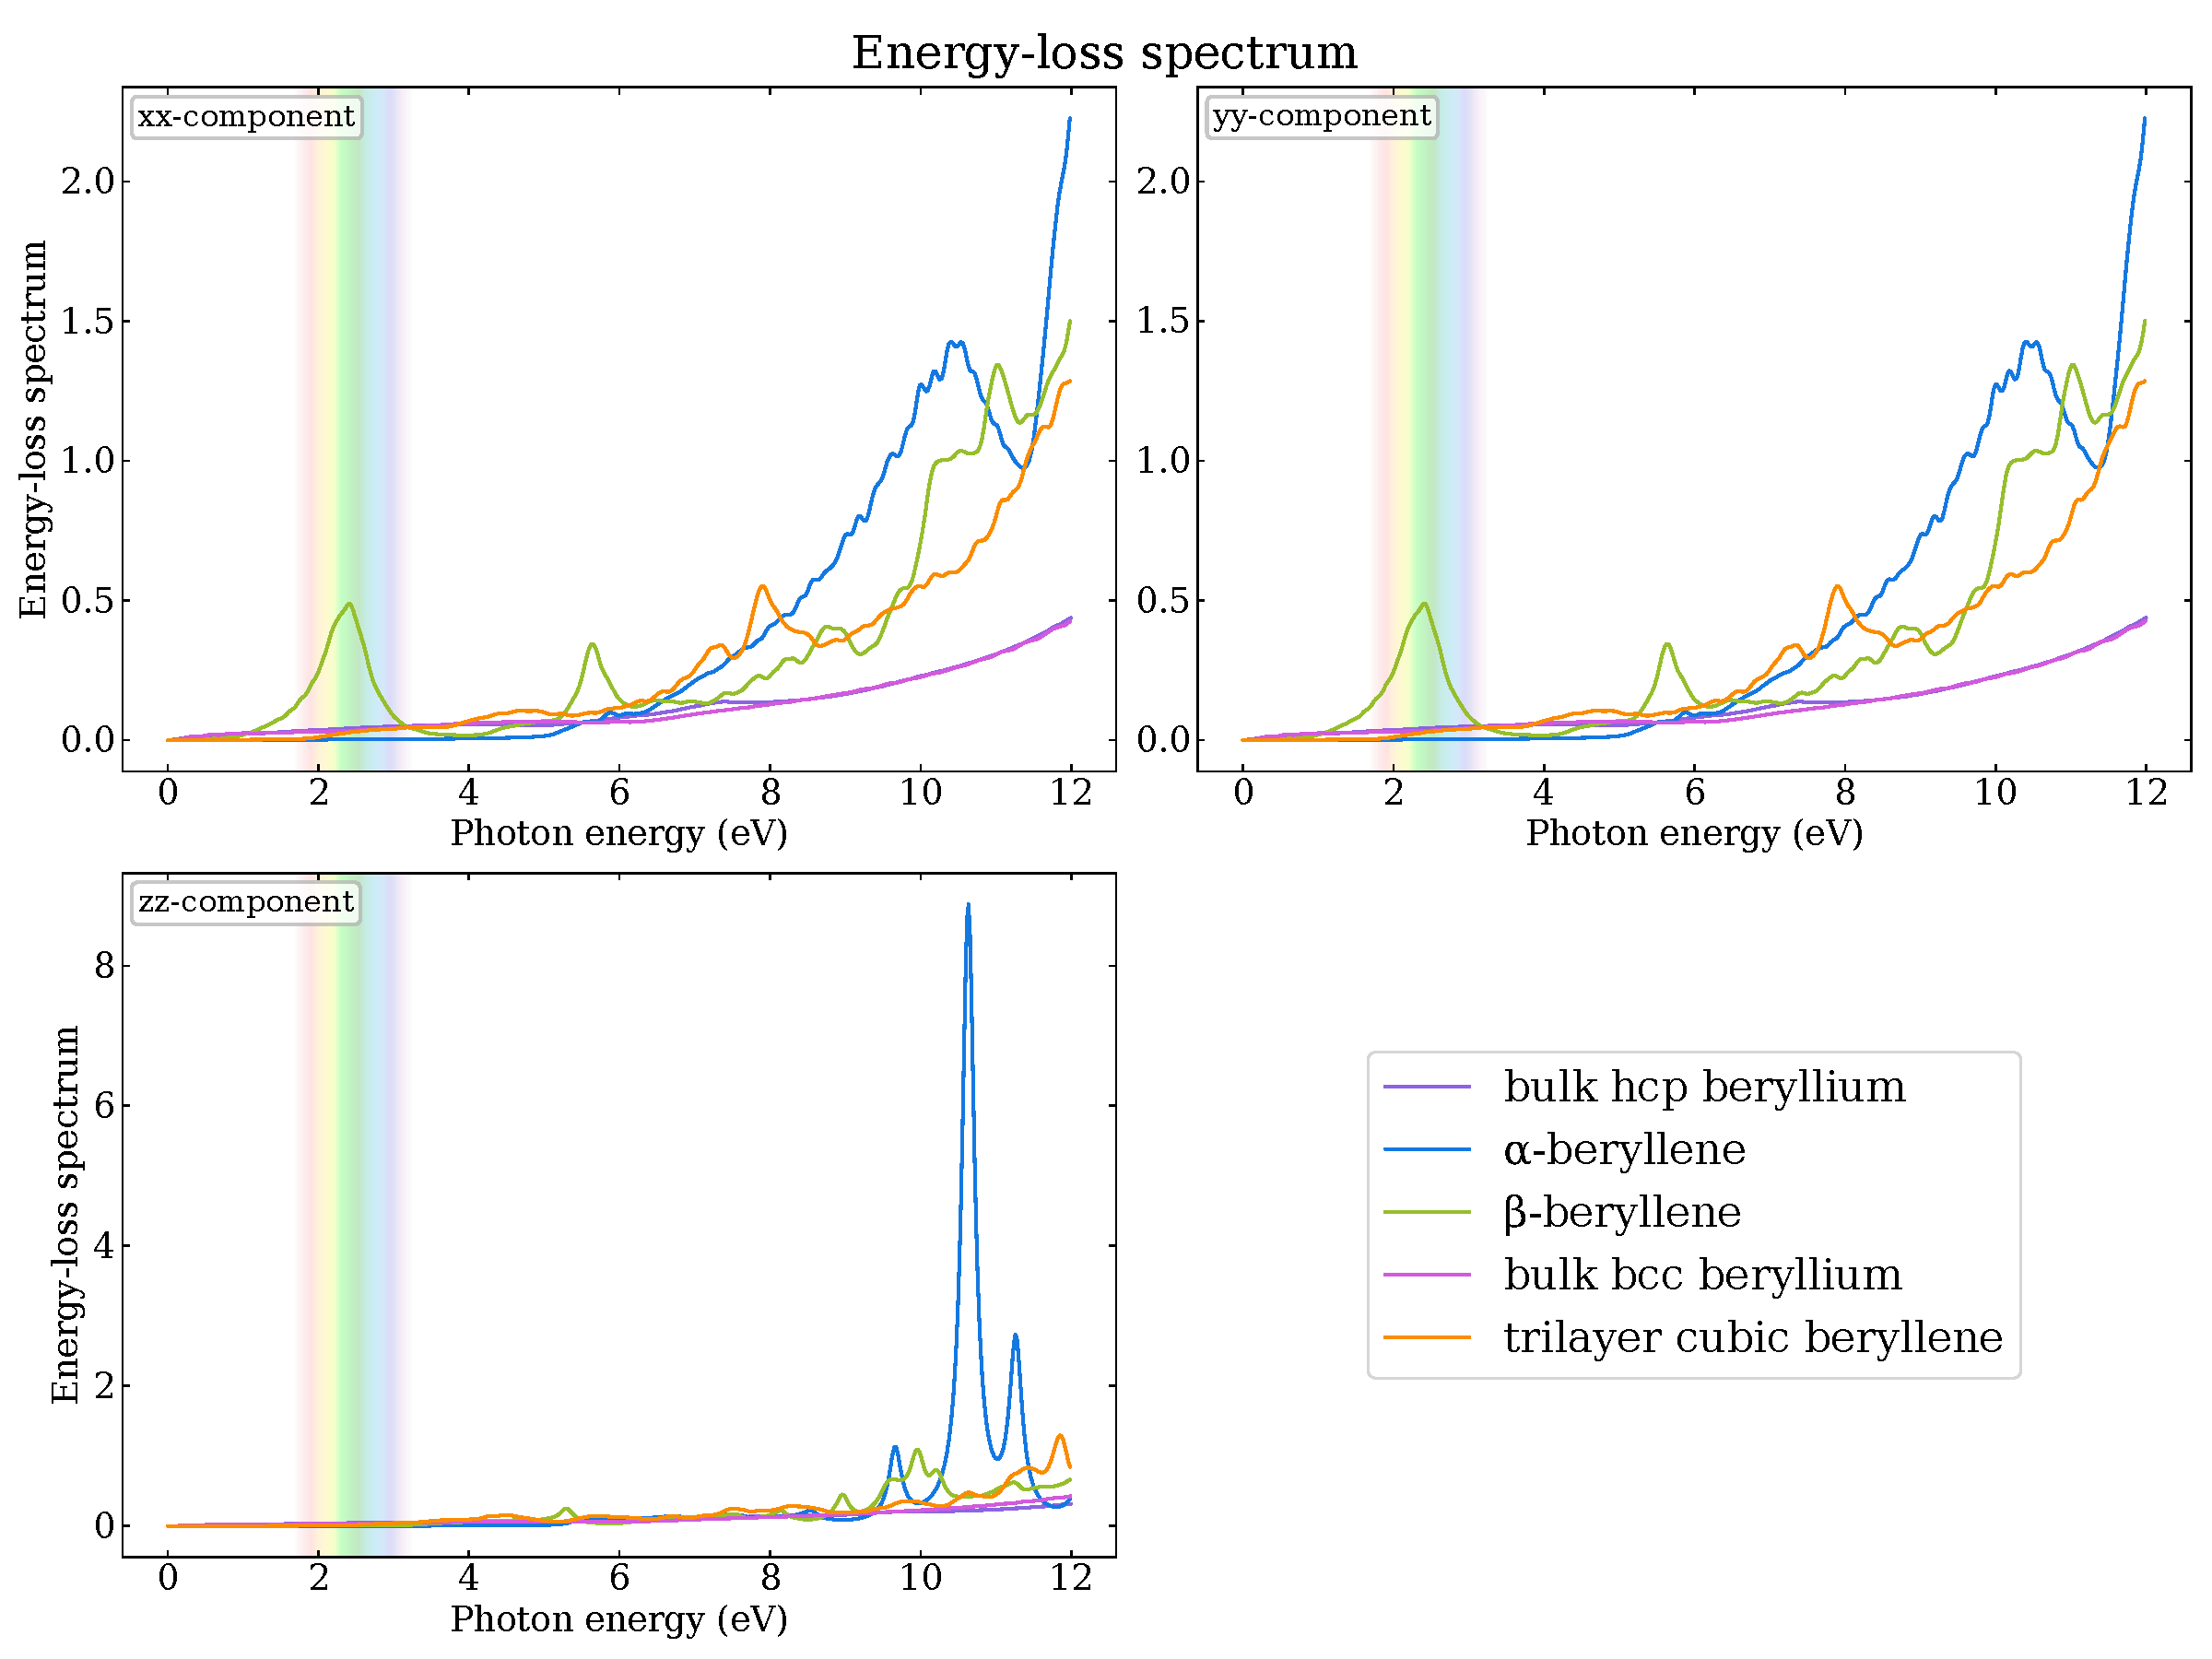
\includegraphics[width=0.80\linewidth]{figures_proj3/optics_pristine_energy-loss_thesis.pdf}}%
\caption{Absorption coefficient and energy-loss spectrum for bulk hcp beryllium,
bulk bcc beryllium,
$\alpha$-beryllene,
$\beta$-beryllene,
and trilayer cubic beryllene.
Upper: absorption coefficient (\unit{\per\nano\metre}). Lower: energy-loss spectrum.
The spectra are shown for the $xx$,
$yy$,
and $zz$ components as functions of photon energy.}
\label{fig:proj3_bulk_cubic_abs_loss}
\end{figure}

\subsubsection{Hydrogen-functionalized beryllene structures}
\label{3_optical_hydrogenated_structures}

We now compare the pristine and hydrogen-functionalized spectra in figure~\ref{fig:proj3_hydrogenated_dielectric}.
For 2H-$\alpha$-beryllene, the real and imaginary components in $xx$ and $yy$ both peak at about 31.2, near \qty{4.91}{\electronvolt} and \qty{5.59}{\electronvolt}, respectively.
In $zz$, the largest imaginary component occurs near \qty{9.77}{\electronvolt}.

Both hydrogen coverages of $\beta$-beryllene give distinct $xx$ and $yy$ responses.
In the double-sided structure, the $xx$, $yy$, and $zz$ imaginary components peak near \qty{6.59}{\electronvolt}, \qty{9.26}{\electronvolt}, and \qty{8.24}{\electronvolt}, respectively.
The corresponding peak heights are 14.96, 7.68, and 14.97.
The first real-part zero crossings occur near \qty{6.65}{\electronvolt}, \qty{9.33}{\electronvolt}, and \qty{8.10}{\electronvolt}, respectively.

\begin{figure}[!htbp]
\centering
    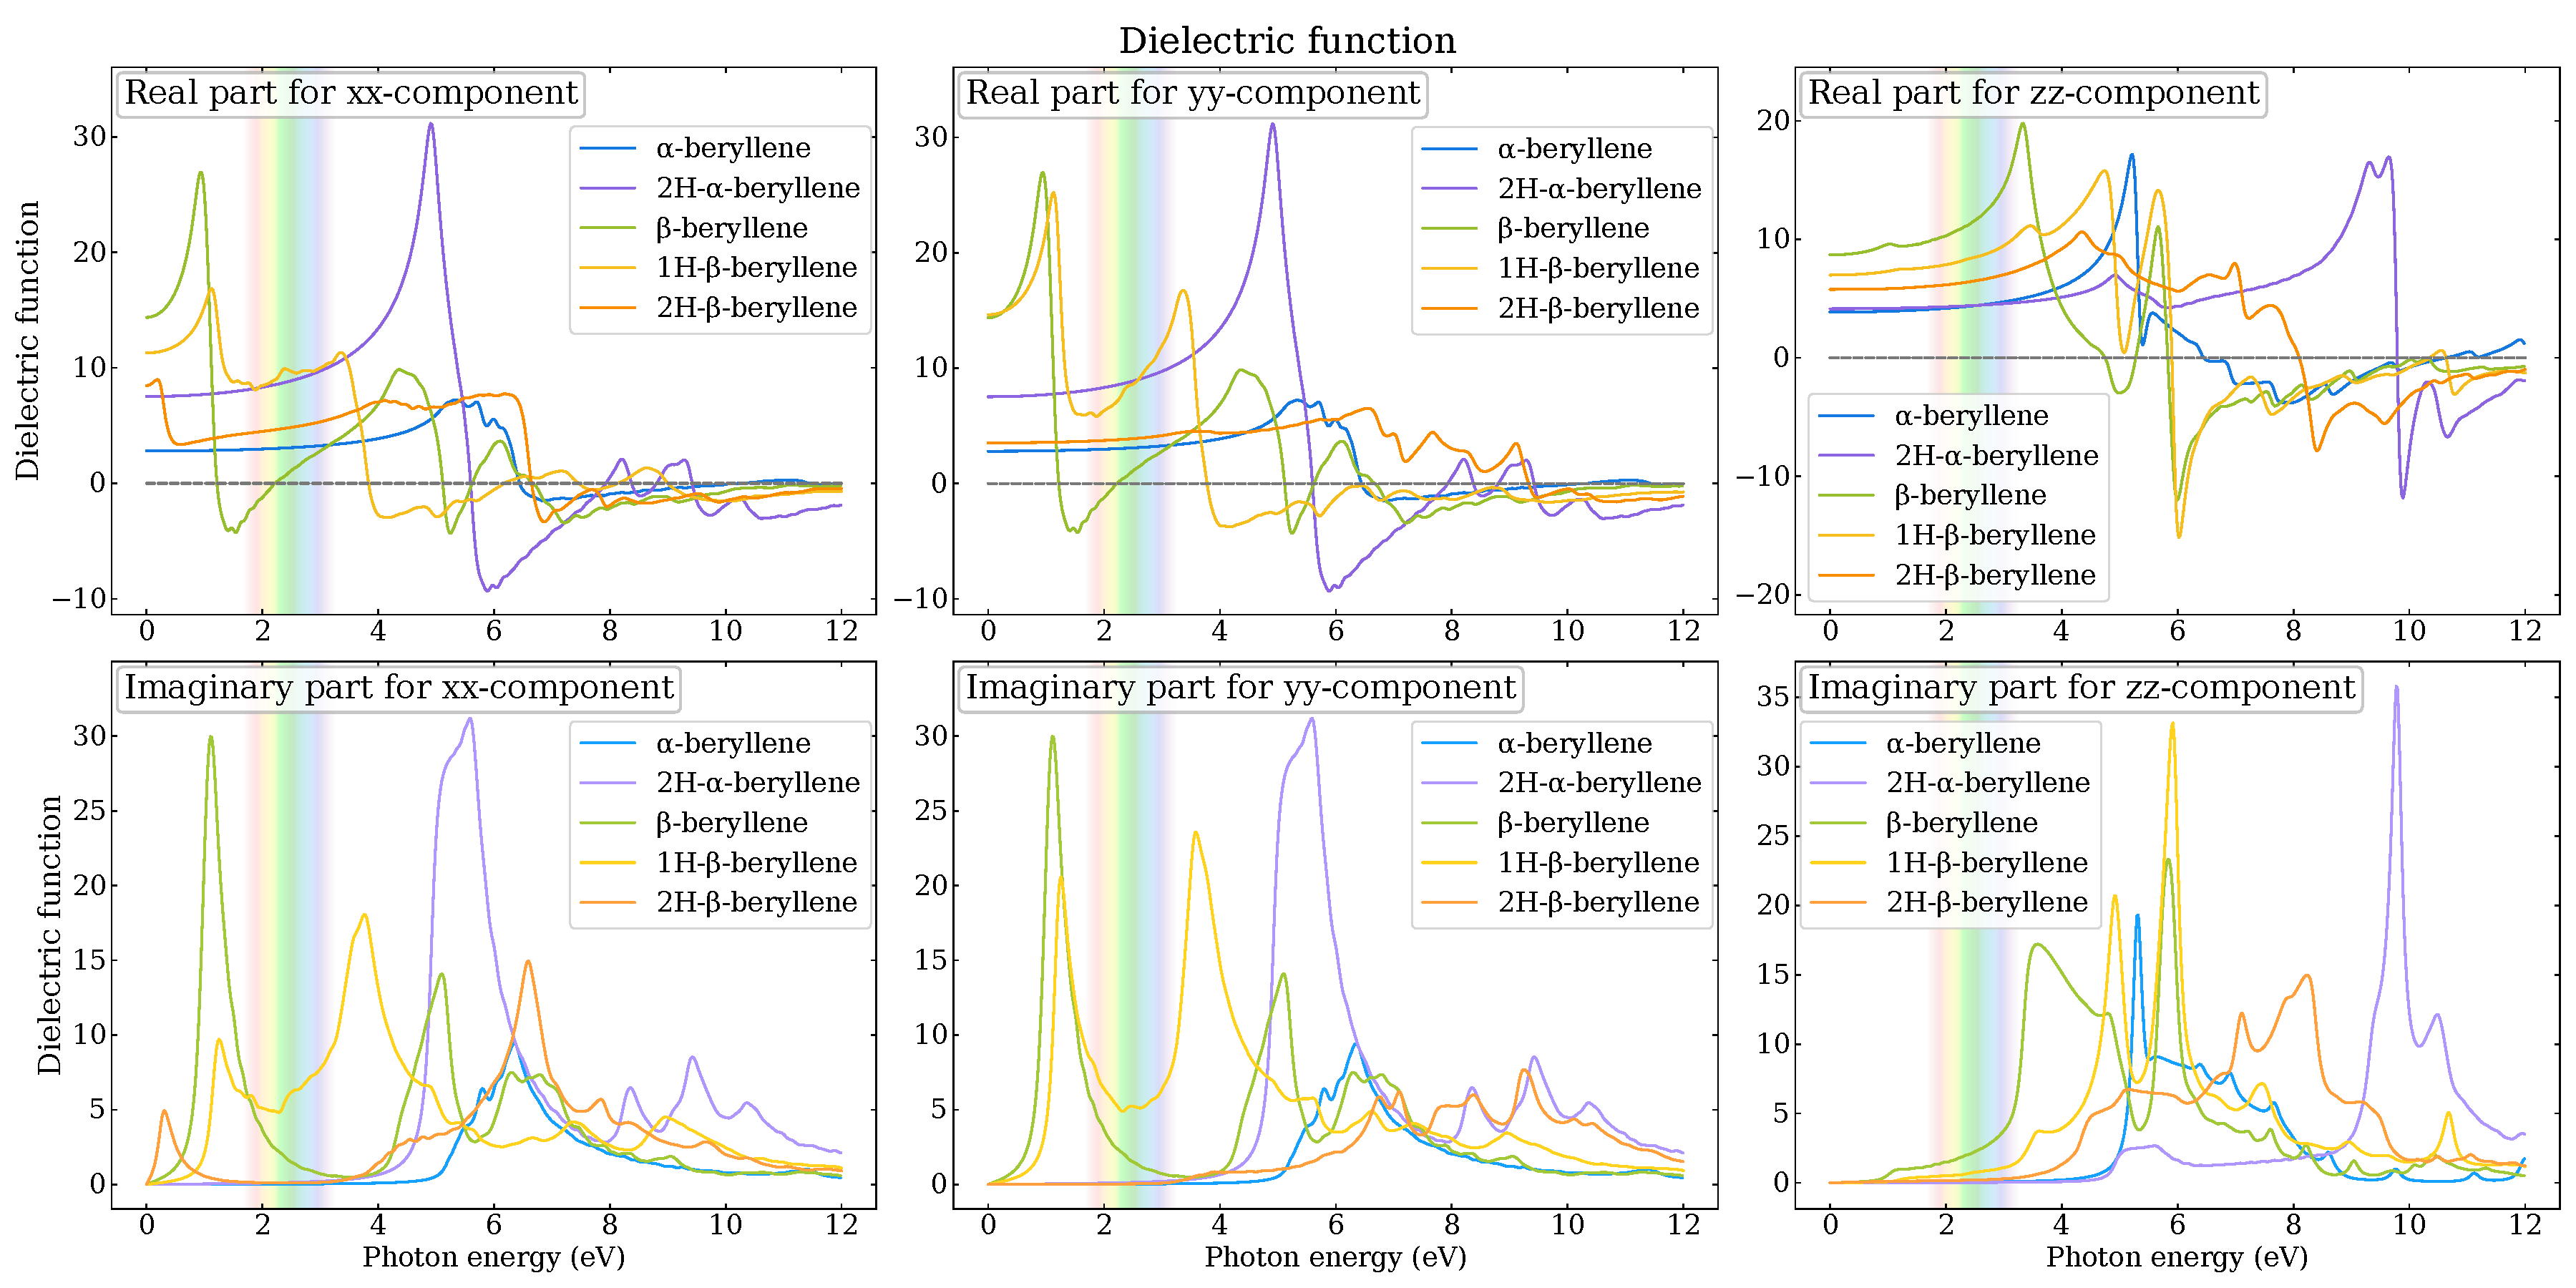
\includegraphics[width=1\linewidth]{figures_proj3/dielectric_hydrogenated_thesis.pdf}
\caption{Real and imaginary parts of the dielectric function for pristine and hydrogen-functionalized $\alpha$- and $\beta$-beryllene structures.
The spectra are shown for the $xx$,
$yy$,
and $zz$ components as functions of photon energy.}
\label{fig:proj3_hydrogenated_dielectric}
\end{figure}

Figure~\ref{fig:proj3_hydrogenated_abs_loss} shows the corresponding absorption and loss spectra.
The absorption coefficients of 2H-$\alpha$-beryllene in $xx$ and $yy$ exceed the pristine values across the sampled visible interval.
Their visible maximum of \qty{0.00137}{\per\nano\metre} is small compared with the ultraviolet maximum of \qty{0.241}{\per\nano\metre} near \qty{5.71}{\electronvolt}.
In $zz$, absorption decreases upon hydrogenation across the sampled \qtyrange{1.65}{4.13}{\electronvolt} interval, and the largest peak moves to \qty{9.83}{\electronvolt}.
Finite broadening gives the PBE spectrum a weak tail below the gap.
The \qty{6.00}{\electronvolt} HSE06 gap is indirect, whereas the calculated optical spectrum samples vertical transitions at fixed wave vector.
For 2H-$\beta$-beryllene, the strongest absorption occurs near \qty{6.75}{\electronvolt} in $xx$, \qty{9.39}{\electronvolt} in $yy$, and \qty{8.36}{\electronvolt} in $zz$.
Hydrogenation also suppresses the strong out-of-plane loss peak of pristine $\alpha$-beryllene near \qty{10.64}{\electronvolt}.

\begin{figure}[!htbp]
\centering
    \adjustbox{valign=c}{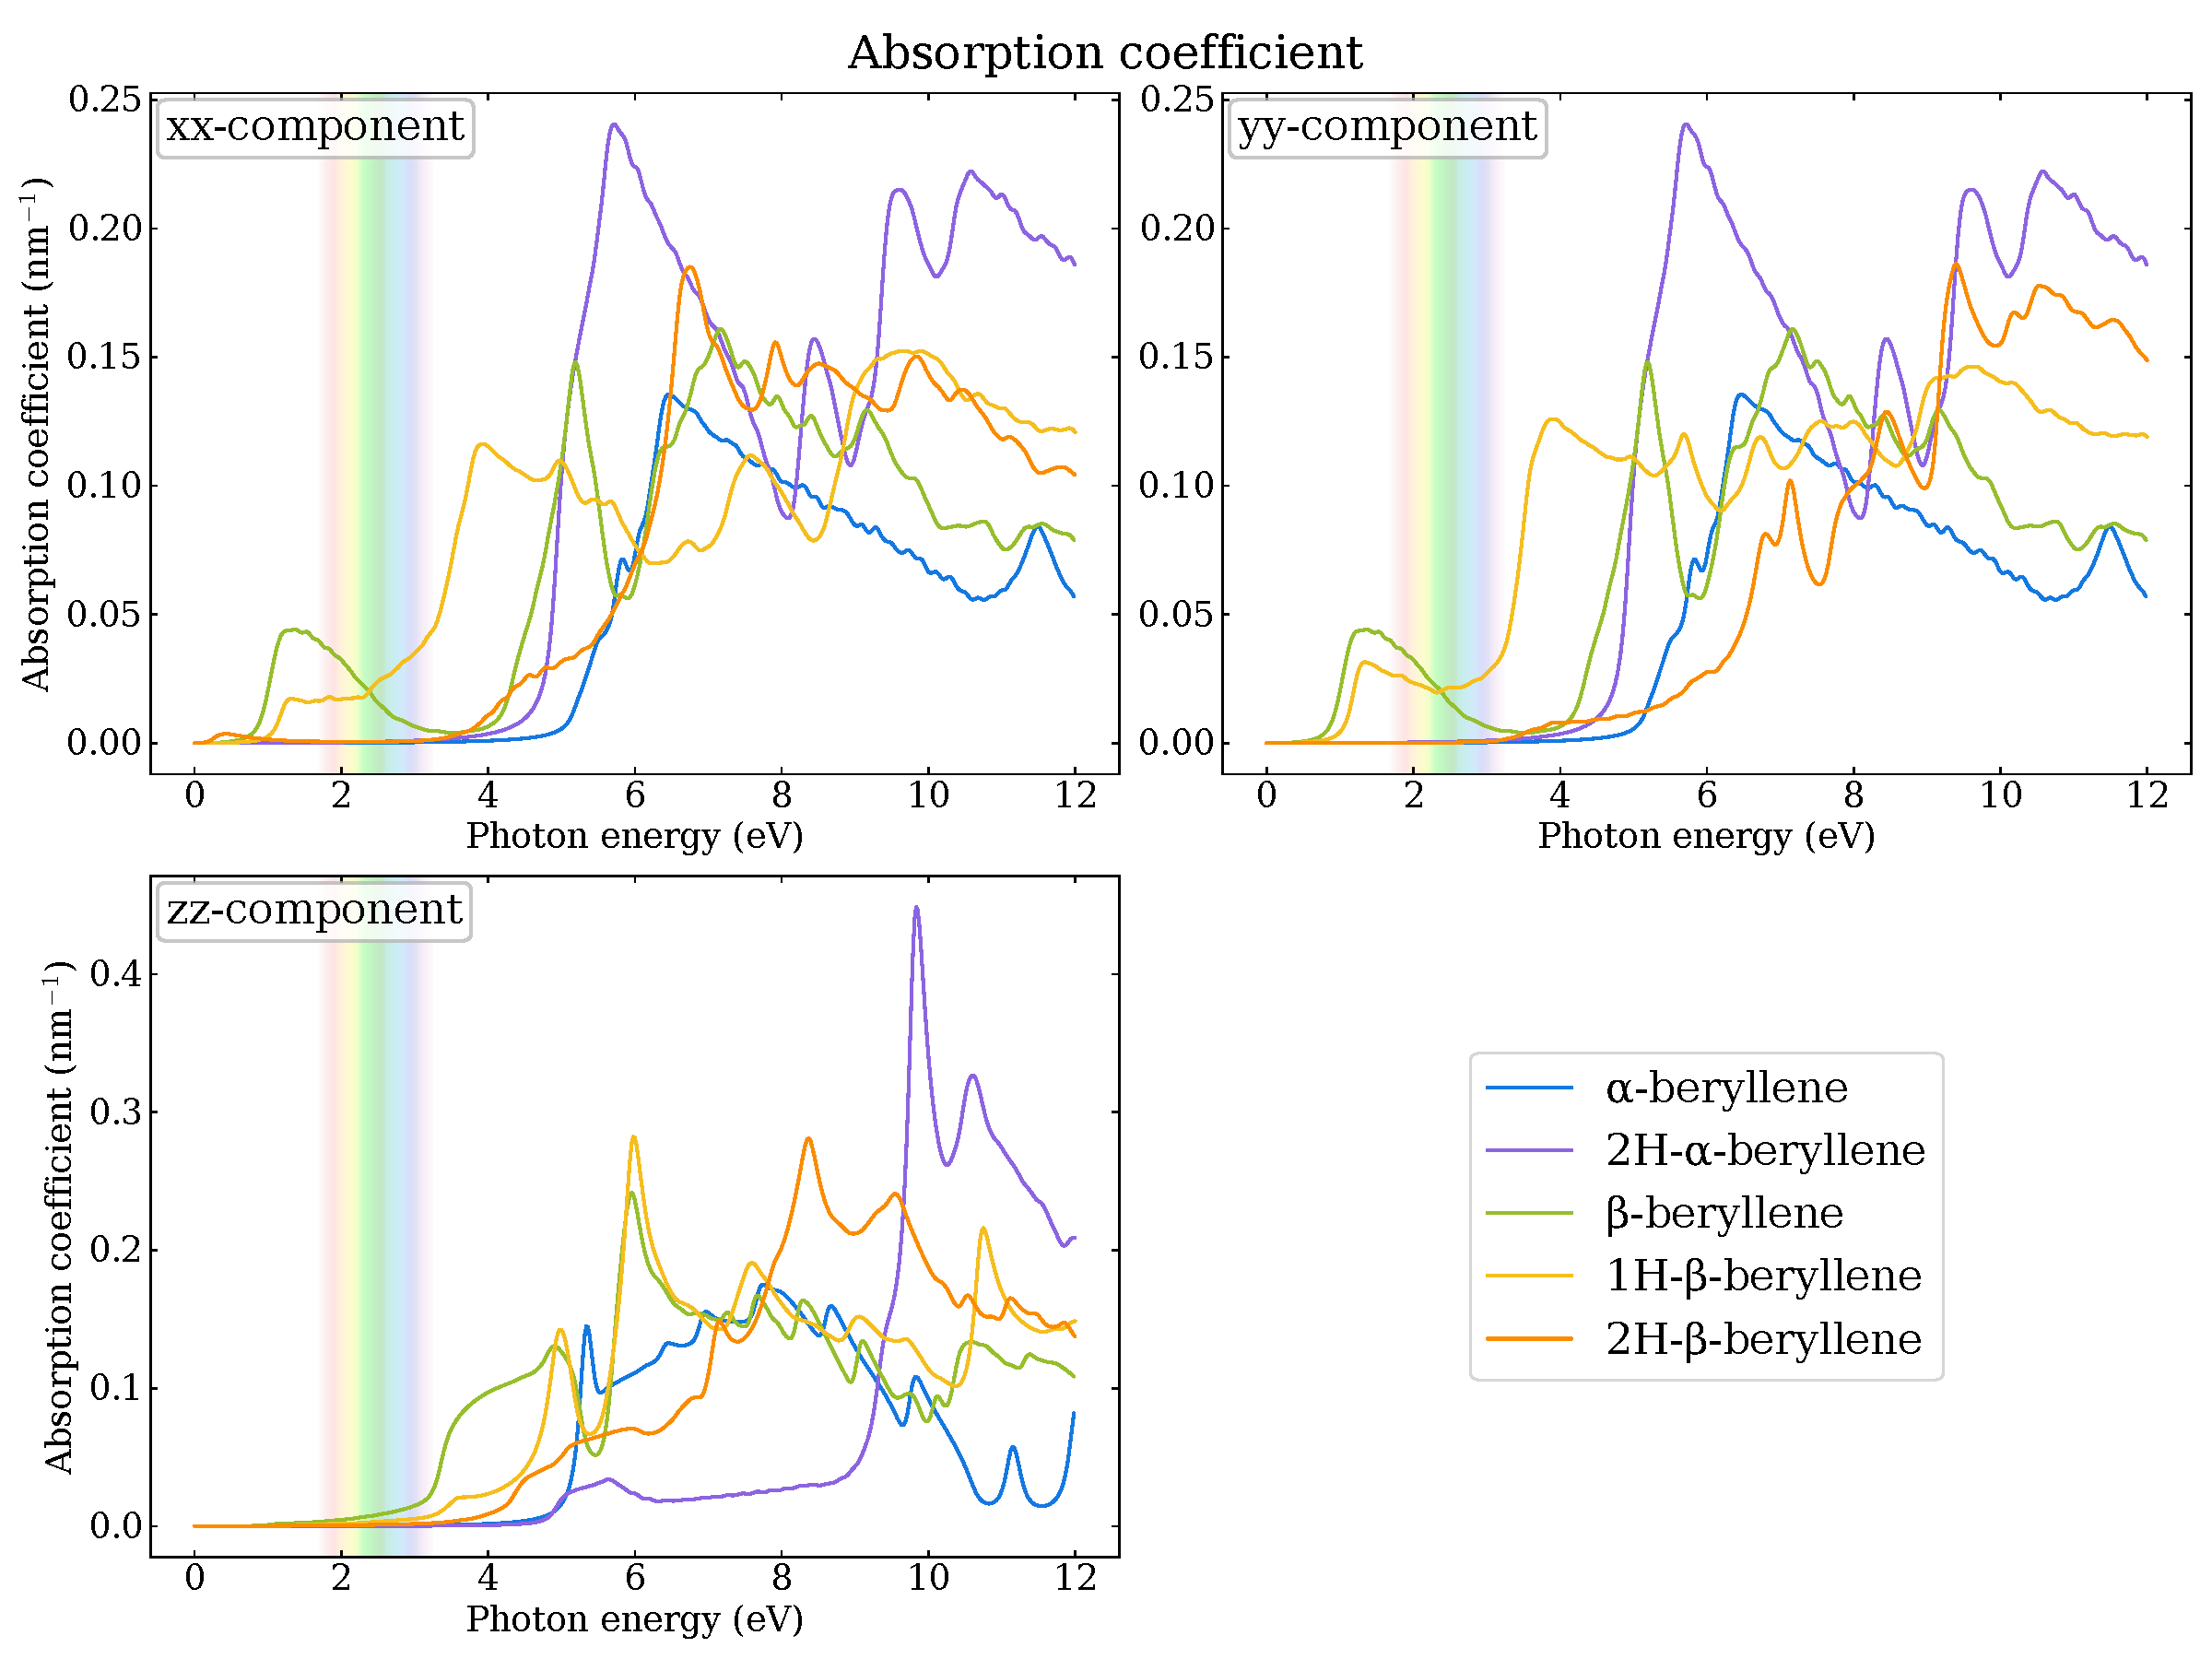
\includegraphics[width=0.80\linewidth]{figures_proj3/optics_hydrogenated_absorption_thesis.pdf}}%
    \par\nointerlineskip
    \adjustbox{valign=c}{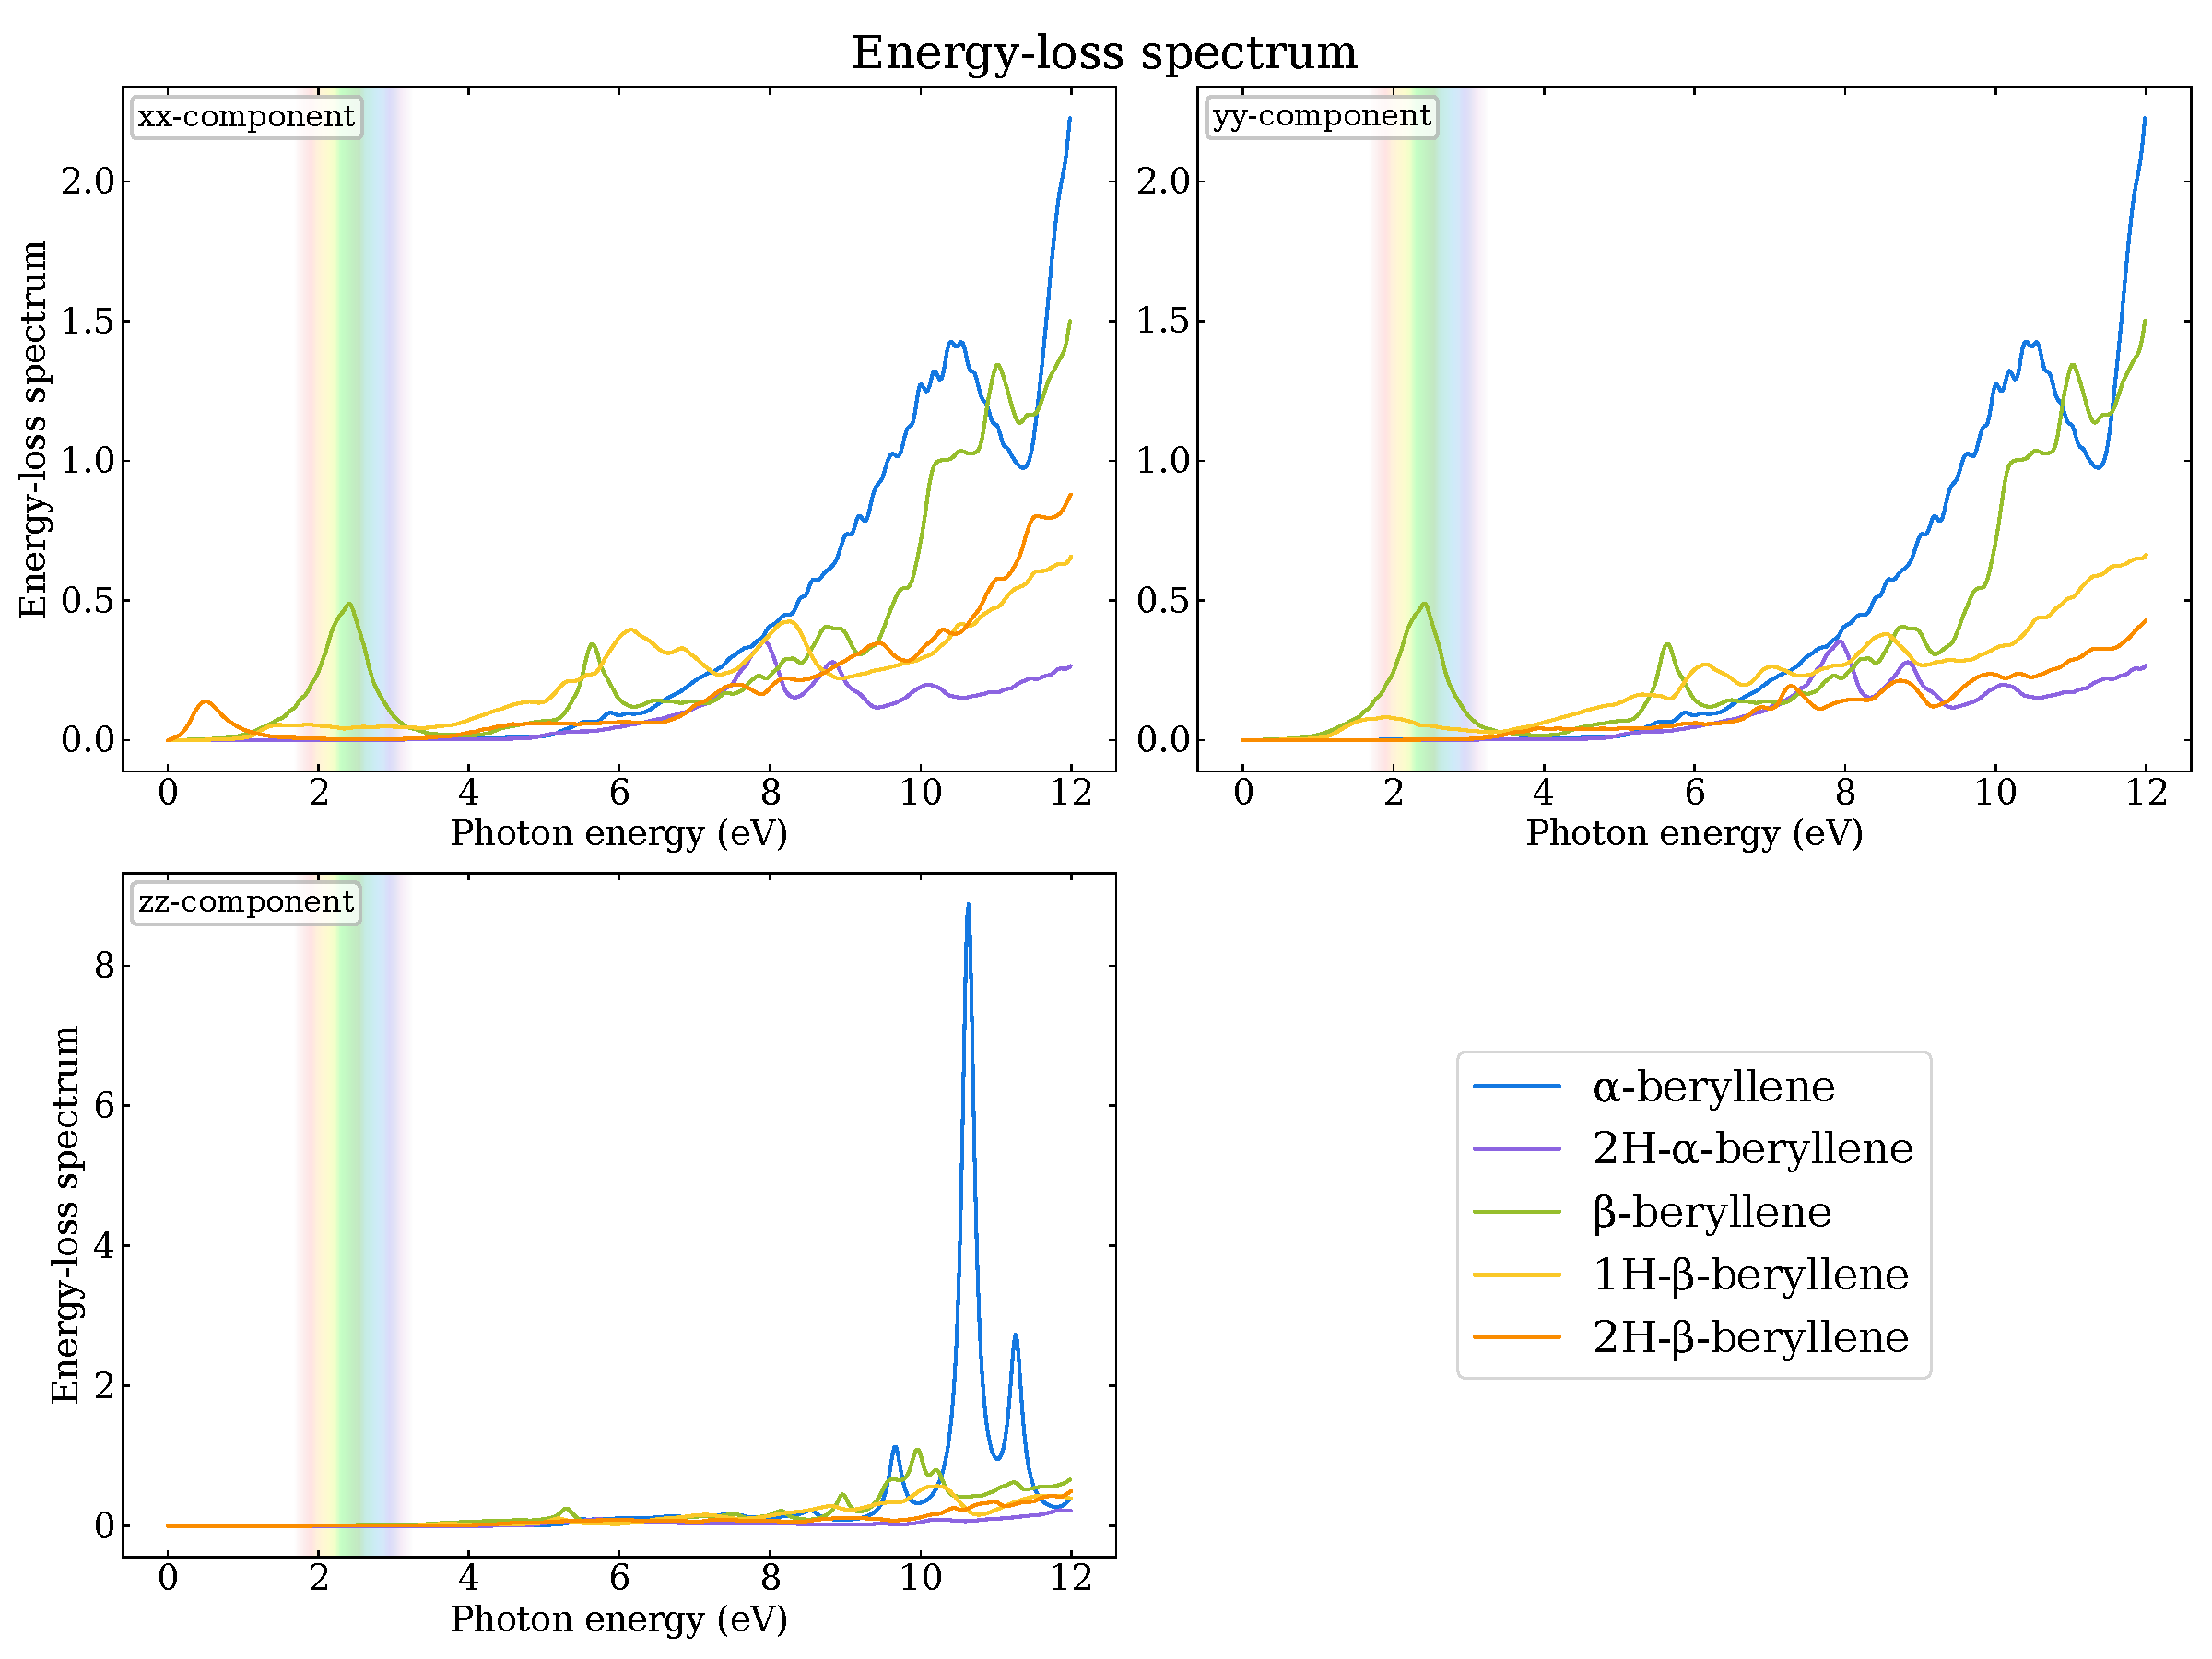
\includegraphics[width=0.80\linewidth]{figures_proj3/optics_hydrogenated_energy-loss_thesis.pdf}}%
\caption{Absorption coefficient and energy-loss spectrum for pristine and hydrogen-functionalized $\alpha$- and $\beta$-beryllene structures.
Upper: absorption coefficient (\unit{\per\nano\metre}). Lower: energy-loss spectrum.
The spectra are shown for the $xx$, $yy$, and $zz$ components as functions of photon energy.}
\label{fig:proj3_hydrogenated_abs_loss}
\end{figure}

\FloatBarrier
\section{Conclusions}
\label{3_conclusions}

The harmonic phonon dispersions support dynamical stability for trilayer cubic beryllene and 2H-$\alpha$-beryllene.
For 1H-$\beta$-beryllene, interpolated imaginary frequencies near $\Gamma$ leave long-wavelength stability unresolved.
The one-mode quantum calculation of 2H-$\beta$-beryllene supports suppression of a static distortion along its soft mode.
All three hydrogenated structures retain their frameworks during \qty{5.5}{\pico\second} at \qty{300}{\kelvin}.

Hydrogenation opens an indirect HSE06 gap of \qty{6.00}{\electronvolt} in 2H-$\alpha$-beryllene, whereas both hydrogenated $\beta$ structures remain metallic.
At \qty{298.15}{\kelvin} and \qty{1}{\bar} of \ce{H2}, only 2H-$\alpha$-beryllene favours adsorption relative to its pristine sheet and gaseous \ce{H2}.
A competing puckered \ce{BeH2} layer has a lower relaxed electronic energy.

The selected subspaces of $\alpha$-beryllene and trilayer cubic beryllene give $\nu=1$, conditional on direct gaps throughout the Brillouin zone.
Their smallest sampled gaps are of order \qty{1}{\milli\electronvolt} and lie well above the Fermi level.
The other selected subspaces give $\nu=0$.

The isotropic Migdal--Eliashberg equations give a transition temperature of \qty{3.7}{\kelvin} for the cubic trilayer.
The anisotropic estimates are approximately \qty{14.2}{\kelvin} for 1H-$\beta$-beryllene and \qty{31.7}{\kelvin} for 2H-$\beta$-beryllene relaxed with the D3 dispersion correction.

Across the sampled visible range, the in-plane absorption coefficient of the cubic trilayer lies below that of bulk bcc beryllium.
Hydrogenation splits the in-plane spectra of $\beta$-beryllene.
In $\alpha$-beryllene, double-sided termination shifts the strongest out-of-plane absorption to \qty{9.83}{\electronvolt} and suppresses the pristine loss peak near \qty{10.64}{\electronvolt}.
